\documentclass[12pt,openany]{book}

% Packages
\usepackage{amsmath} % For advanced math formatting (e.g., \max, \min, and align environments)
\usepackage{amssymb}  % math symbols
\usepackage{array}   % For advanced table formatting
\usepackage{booktabs} % For professional-looking tables
\usepackage{caption}  % For positioning table and figure descriptions.
\usepackage{color, xcolor} % For colored shading
\usepackage{etoolbox}  % stops LaTeX from trying to make pages look "full" by spacing everything out
\usepackage{fancyhdr}
\usepackage{float}
\usepackage{graphicx} % For including arrows and images.
\usepackage{helvet} % For Helvetica font
\usepackage{hyperref} % For clickable table of contents
\usepackage[top=1in, bottom=1in, left=0.75in, right=0.75in]{geometry}
\usepackage{mdframed}
% \usepackage{sectsty}
\usepackage{pifont}
\usepackage{pgfplots}
\usepackage{titlesec} % For customizing section and chapter titles
\usepackage{tikz}
\usepackage{xcolor}


\pgfplotsset{compat=1.18}  

\newcommand{\cmark}{{\color{green!60!black}\ding{51}}} % checkmark
\newcommand{\xmark}{{\color{red!80!black}\ding{55}}}   % cross



\captionsetup[table]{position=above}
\captionsetup[figure]{position=below}

\raggedbottom


\usetikzlibrary{arrows.meta, positioning}
\usetikzlibrary{shapes.geometric, arrows}


\renewcommand{\familydefault}{\sfdefault} % Set sans-serif as default font family

% Set up minimal fancy footer for page numbers
\pagestyle{fancy}
\fancyhf{} % Clear all headers and footers
\fancyfoot[C]{\thepage} % Page number centered in the footer


% Define custom header style
\renewcommand{\chaptermark}[1]{%
  \markboth{\textcolor{gray!60}{\MakeUppercase{#1}}}{}%
}

% Customize headers
\fancyhead{} % Clear all headers
\fancyhead[L]{%
  \vspace*{-8mm} 
  \colorbox{gray!20}{%
    \parbox{\dimexpr\textwidth-3.2mm}{
      \textbf{\leftmark}
    }
  }%
}
\fancyhead[C]{} % Remove the horizontal line
\fancyhead[R]{} % Optional: Leave this empty or add something else
\pagestyle{fancy}

% Define the example environment
\newmdenv[
  backgroundcolor=gray!10, % Light gray background
  linecolor=gray!50, % Border color
  linewidth=1pt, % Border thickness
  roundcorner=5pt, % Rounded corners
  skipabove=10pt, % Space above the example
  skipbelow=10pt, % Space below the example
  innertopmargin=5pt, % Inner top margin
  innerbottommargin=5pt, % Inner bottom margin
  innerleftmargin=10pt, % Inner left margin
  innerrightmargin=10pt, % Inner right margin
  frametitlefont=\bfseries, % Title font style
  frametitle={Example}, % Title text
]{examplebox}
% Write like this:
% \begin{examplebox}
% This is an example box. Use it to illustrate key concepts, provide practical use cases, or demonstrate % step-by-step workflows relevant to the text.
% \end{examplebox}
% Maximum is a single paragraph.


% Define the Note box environment
\newmdenv[
  backgroundcolor=blue!5, % Light blue background
  linecolor=blue!50, % Blue border color
  linewidth=1pt, % Border thickness
  roundcorner=3pt, % Slightly rounded corners
  skipabove=10pt, % Space above the box
  skipbelow=10pt, % Space below the box
  innertopmargin=5pt, % Inner top margin
  innerbottommargin=5pt, % Inner bottom margin
  innerleftmargin=10pt, % Inner left margin
  innerrightmargin=10pt, % Inner right margin
  frametitlefont=\itshape, % Italic font style for the title
  frametitle={Note}, % Title text
]{notebox}
% Write like this:
% \begin{notebox}
% This is an important note for readers. Use it to highlight additional context, tips, or cautions.
% \end{notebox}
% Maximum is a single paragraph, that should be kept very short. Use notes only sparingly.


% Define the Summary box environment
\newmdenv[
  backgroundcolor=green!5, % Light green background
  linecolor=green!50, % Green border color
  linewidth=1pt, % Border thickness
  roundcorner=5pt, % Rounded corners
  skipabove=10pt, % Space above the box
  skipbelow=10pt, % Space below the box
  innertopmargin=5pt, % Inner top margin
  innerbottommargin=5pt, % Inner bottom margin
  innerleftmargin=10pt, % Inner left margin
  innerrightmargin=10pt, % Inner right margin
  frametitlefont=\bfseries, % Bold title font style
  frametitle={Summary}, % Title text
]{summarybox}
% Write like this:
% \begin{summarybox}
% \begin{itemize}
%   \item This is a summary point. Keep it concise and informative.
%   \item Use only a few bullet points to summarize key ideas.
%   \item Avoid lengthy explanations; focus on brevity and clarity.
% \end{itemize}
% \end{summarybox}
% Maximum is a few bullet points, ideally 3–5.
% Use the summary box sparingly to highlight essential takeaways for sections or chapters.



\tikzstyle{startstop} = [rectangle, rounded corners, minimum width=3cm, minimum height=1cm,text centered, draw=black, fill=red!30]
\tikzstyle{process} = [rectangle, minimum width=3cm, minimum height=1cm, text centered, draw=black, fill=blue!30]
\tikzstyle{arrow} = [thick,->,>=stealth]


% No paragraph indentation
\setlength{\parindent}{0pt}

% Blue level headers ------------------------------------------------------------------------------
% Part headers (centered, dark blue)
\titleformat{\part}[display]
  {\Huge\bfseries\color{blue!80}\filcenter} % Dark blue, centered
  {\partname~\thepart}
  {0.5em}
  {\vspace*{1in}} % Push part header to middle of the page

% Chapter headers (dark blue, left-aligned)
\titleformat{\chapter}[display]
  {\Huge\bfseries\color{blue!80}}
  {\chaptername~\thechapter}
  {0.5em}
  {\vspace{1em}} % Small spacing after chapter number

% Section headers (lighter blue)
\titleformat{\section}[hang]
  {\Large\bfseries\color{blue!60}}
  {\thesection}
  {1em}
  {}

% Subsection headers (even lighter blue)
\titleformat{\subsection}[hang]
  {\large\bfseries\color{blue!50}}
  {\thesubsection}
  {1em}
  {}

% Subsubsection headers (lightest blue)
\titleformat{\subsubsection}[hang]
  {\bfseries\color{blue!40}}
  {\thesubsubsection}
  {1em}
  {}

% Remove indentation
\setlength{\parindent}{0pt}
% ----------------------------------------------------------------------------------------



% Feedback from Nik: 
% - Title to the notes, and it is not clear when to use a note and when not --> true
% - Always write this summary, and actually put it in the beginning, not at the end.
% - Make gen set more clear --> take his example, indluce it, and say this would not be a good gen
% set, because its another task, it would be unfair. Better would be another dialect of English.

\setlength\emergencystretch{5em}  % allow TeX to fix bad lines
\hfuzz=1.5pt                      % ignore small overflows outside paragraphs
\hbadness=10000                  % suppress low-severity badness messages
\AtBeginDocument{\sloppy}       % global sloppy mode


\begin{document}

\begin{titlepage}
    \centering
    \newpage
    \thispagestyle{empty}
    
    \begin{tikzpicture}[remember picture, overlay]
        \fill[violet] (current page.south west) rectangle (current page.north east);
    \end{tikzpicture}
    
    \vspace*{2cm}
    {\LARGE \textbf{\textcolor{white}{Decision Making in Machine Learning Projects:}}} \\
    \vspace{0.5cm}
    {\LARGE \textbf{\textcolor{white}{From Scoping to Deployment}}} \\

    
    \vspace{2cm}  % Adjusted spacing for better balance
    \Large{\textcolor{white}{\textbf{Thomas Rauter}}} \\
    
    \vspace{0.5cm}
    \large{\textcolor{white}{Version 0.2.1}} \\
    \large{\textcolor{white}{22.03.2025}} \\
    
    \vspace{1.5cm}
    \includegraphics[width=0.7\textwidth]{general_figures/cover_page_image.png} \\
    
    \vfill
    \small{\textcolor{white}{This document is based on ideas developed by Andrew Ng, with extensions and additional content written by Thomas Rauter. The publicly shared material has been adapted and expanded upon in accordance with its intended use for educational purposes.}} 
    
\end{titlepage}


% Set Table of Contents depth
\setcounter{tocdepth}{1}

% Table of Contents
\tableofcontents

\newpage

\section{Purpose and Audience}

\begin{center}
\textit{This book will tell you \textcolor{green!50!black}{\textbf{what}} to do, \textcolor{green!50!black}{\textbf{when}} to do it, and \textcolor{green!50!black}{\textbf{why}}—\\
but if you want to know \textcolor{red!70!black}{\textbf{how}}, or dive into the \textcolor{red!70!black}{\textbf{details}}, you must consider additional resources.}
\end{center}

\vspace{1em}
\textbf{About:}

% First list: What, When, Why (green)
\begin{itemize}
    \item \textcolor{green!50!black}{\textbf{What:}} Know what tools, methods, and techniques exist. Awareness is the foundation of good decisions—if you don’t know something exists, you’ll never consider it.
    \item \textcolor{green!50!black}{\textbf{When:}} Knowing when to apply something is the essence of practical skill.
    \item \textcolor{green!50!black}{\textbf{Why:}} Provides the hook that turns knowledge into judgment.
\end{itemize}

\vspace{1em}
\textbf{Not about:}

% Second list: How, Details (red)
\begin{itemize}
    \item \textcolor{red!70!black}{\textbf{How:}} Refers to implementation—code and tutorials.
    \item \textcolor{red!70!black}{\textbf{Details:}} Refers to in-depth theoretical explanations, such as the mathematical foundations of neural networks.
\end{itemize}
% Code and tutorials gets outdated more quickly than general knowledge, and therefore needs maintenance. Further, there are many online resources that provide this. For this reason, it is not covered in this book, to make it more concise.
% For the details there also exist many resources, in the form of books, free online articles, or online courses.


This document is intended for practitioners who already possess a 
solid understanding of machine learning fundamentals. This book focuses on the decision-making process throughout the machine learning workflow, from scoping to deployment.



\section{Terminology}

To ensure consistency and clarity throughout this document, the following terms will always be used in preference to alternative expressions for the same concepts:

\begin{itemize}
    \item \textbf{Dev set:} Refers to the validation or development set used during model evaluation and hyperparameter tuning. The model is not trained on this data, rather, it is used to asses how well the model performs on unseen data. During development, the dev set is used for this to avoid overfitting the hyperparameters to the test set.
    \item \textbf{Instances:} Refers to the individual rows of a dataset, also known as observations, examples, or samples. 
\end{itemize}


% Introduction
\section{Introduction}

Machine learning projects follow a structured workflow, from defining project goals to deploying and maintaining the final system. This workflow can be broadly divided into four interconnected stages: \textbf{Scoping}, where project objectives and constraints are defined; \textbf{Data}, where data is (collected), explored, cleaned, split, and changed to improve model performance; \textbf{Modeling}, where algorithms are used to train models; and \textbf{Deployment}, where models are integrated into production systems and monitored for continued success. Figure~\ref{fig:ml_project_overview} provides an overview of this workflow, highlighting the key steps within each stage.

\begin{figure}[H]
    \centering
    \includegraphics[width=1\textwidth]{./general_figures/ml_project_overview.png}
    \caption{Overview of the machine learning workflow: Scoping, Data, Modeling, and Deployment. While these steps are generally carried out sequentially, iterative refinement is often required to optimize outcomes.}
    \label{fig:ml_project_overview}
\end{figure}

Throughout the machine learning workflow, countless decisions shape the success of a project. \textbf{Scoping} involves choosing the right problems to tackle—should you focus on improving product recommendations or optimizing inventory management? Some problems carry much higher impact than others. In the \textbf{data} stage, you must decide what to look for, how to split the data, whether to remove outliers, and how best to represent the data for your model. During \textbf{modeling}, you face questions about model selection, diagnosing performance issues, and figuring out what to do when the results still fall short. Finally, in \textbf{deployment}, you need to select a deployment strategy and ensure your model continues to perform reliably in the real world. This ebook is here to help you navigate these decisions and make choices that actually move the needle. 
\newline

\begin{examplebox}
A data science team at a mid-sized retail company was tasked with "improving operations using AI." Without clearly scoping the problem, they jumped straight into modeling, deciding to predict future sales using historical transaction data. They spent months building a complex deep learning model—only to realize late that the business actually needed better inventory management, not sales prediction. Their data was full of inconsistencies, but they cleaned it based on intuition instead of involving domain experts. Their test set was drawn from a different time period than their deployment setting, leading to misleadingly good offline performance. Once deployed, the model failed catastrophically—stockouts increased, inventory costs soared, and customer complaints piled up. Leadership lost confidence in the entire data team, and the initiative was quietly shelved. Hundreds of hours of work were wasted because poor decisions were made throughout the project.
\end{examplebox}


This is a fictional example, and we don’t believe data science projects usually go this wrong—or that you’re reading this book because this applies to you. However, we do hope this book helps you to become an even more effective data scientist.
\newline


The chapters are organized as follows:
\begin{itemize}
    \item \textbf{Scoping:} Strategies for identifying and prioritizing impactful projects and setting clear objectives.
    \item \textbf{Data:} Exploratory data analysis, cleaning, augmentation, feature engineering, and dataset splitting
    \item \textbf{Modeling:} Choosing a model class, objective function, optimizer, and evaluation metric, choosing training strategies, diagnosing errors, and auditing model performance in a structured, practical way.
    \item \textbf{Deployment:} Best practices for integrating models into production and monitoring them.
\end{itemize}



\part{Scoping}

\section*{Introduction to the Scoping Stage}

Picking the right project to work on is one of the most critical and valuable skills in machine learning. Of all the potential ideas you could work on, some will be considerably more valuable than others—perhaps two, five, or even ten times more impactful. Scoping helps ensure that you select the most valuable project to maximize the impact of your work, rather than spreading resources across less meaningful tasks. By carefully considering feasibility, value, and alignment with business goals, scoping prevents wasted effort and directs focus toward high-impact opportunities. \newline

As shown in Figure~\ref{fig:scoping_stage}, scoping is the first step in the broader machine learning workflow. It lays the foundation for the entire project by defining objectives, success metrics, and resource needs, ensuring that all subsequent stages, such as Data, Modeling, and Deployment, are aligned with the project’s goals. This structured approach ensures that the time and effort invested lead to meaningful outcomes.


\begin{figure}[htbp]
    \centering
    \includegraphics[width=1\textwidth]{./scoping_figures/scoping_stage.png}
    \caption{The Scoping stage in the machine learning project workflow.}
    \label{fig:scoping_stage}
\end{figure}

\begin{examplebox}
Consider an ecommerce retailer aiming to increase sales. During the scoping stage, you might brainstorm a variety of business problems, such as:
\begin{itemize}
    \item Developing a better recommender system.
    \item Improving search functionality so users can find products more easily.
    \item Enhancing catalog data by filling in missing fields or correcting inaccuracies.
    \item Optimizing inventory management to decide how many items to stock or where to ship them.
    \item Implementing price optimization strategies to maximize profits.
\end{itemize}
However, not all ideas are equally impactful, and resources are finite. Key questions to answer during this process include:
\begin{itemize}
    \item What project should we work on?
    \item What are the metrics for success?
    \item What resources (data, time, people) are needed to execute this project?
\end{itemize}
This emphasizes the importance of focusing on the most valuable ideas, as selecting the right project can considerably enhance the impact of your efforts.
\end{examplebox}

\chapter{Scoping Process}

The scoping process is a structured framework for identifying and prioritizing machine learning projects, ensuring that efforts are focused on initiatives with the greatest potential impact. It provides a clear sequence of steps that guide teams from understanding business needs to planning actionable solutions, helping to avoid wasted resources on low-impact or infeasible projects. \newline

As illustrated in Figure~\ref{fig:scoping_process}, the process consists of five interconnected steps. Starting with brainstorming business problems, the process progresses through generating AI solutions, assessing feasibility and value, determining milestones, and finally budgeting for resources. Each step builds upon the previous one, ensuring a logical flow from problem identification to actionable project planning. 


\begin{figure}[htbp]
\centering
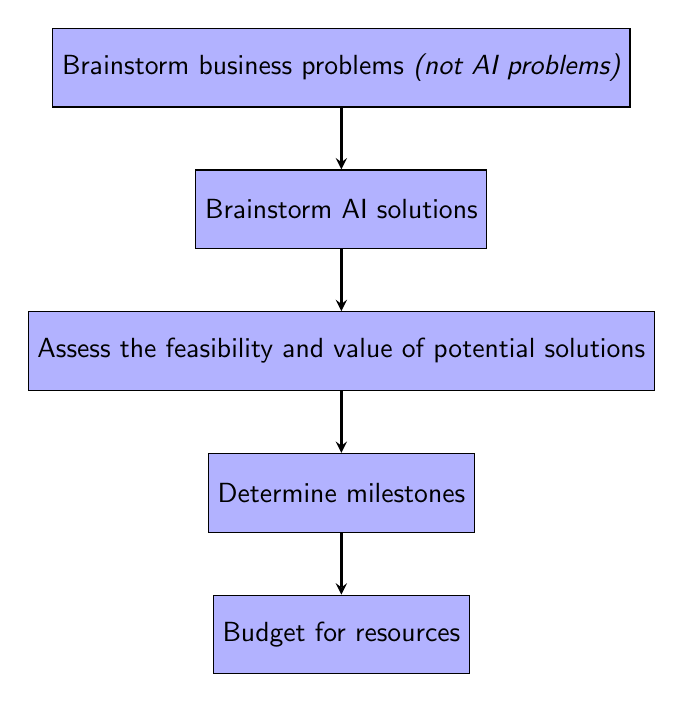
\begin{tikzpicture}[node distance=1.8cm]

% Nodes
\node (problem) [process] {Brainstorm business problems \textit{(not AI problems)}};
\node (solution) [process, below of=problem] {Brainstorm AI solutions};
\node (feasibility) [process, below of=solution] {Assess the feasibility and value of potential solutions};
\node (milestones) [process, below of=feasibility] {Determine milestones};
\node (budget) [process, below of=milestones] {Budget for resources};

% Arrows
\draw [arrow] (problem) -- (solution);
\draw [arrow] (solution) -- (feasibility);
\draw [arrow] (feasibility) -- (milestones);
\draw [arrow] (milestones) -- (budget);

\end{tikzpicture}
\caption{Overview of the scoping process.}
\label{fig:scoping_process}
\end{figure}


\section{Brainstorm Business Problems}

The foundation of any successful machine learning project begins with identifying the key business problems it aims to address. This step focuses on understanding the organization's needs and challenges, rather than diving directly into potential AI solutions.
\newline

To begin, it is essential to collaborate with business or product owners who have a deep understanding of the application domain. These stakeholders can articulate the primary objectives or pain points the organization faces, such as improving user experience, reducing operational inefficiencies, or increasing revenue. Importantly, the focus should remain on framing these challenges as business problems, not AI problems. This underscores the importance of domain knowledge in data science, as it enables practitioners to both understand stakeholders' perspectives and operate independently when access to those stakeholders is limited.
\newline

For example, in the context of an ecommerce retailer, common business problems might include:
\begin{itemize}
    \item Increasing conversion rates by ensuring users find what they are looking for.
    \item Reducing inventory by accurately predicting demand.
    \item Improving profit margins by optimizing pricing strategies or bundling products effectively.
\end{itemize}

This separation between problem identification and solution generation is critical. By clearly articulating the desired outcomes in business terms, teams can ensure alignment with organizational goals. Furthermore, this approach lays a strong foundation for brainstorming AI solutions in the next phase of the scoping process.


\section{Brainstorm AI Solutions}

After identifying the key business problems, the next step is to explore potential AI solutions that could address these challenges. This phase involves mapping the business objectives to technical possibilities and evaluating whether machine learning can effectively contribute to solving the problem.
\newline

It is important to approach this step collaboratively, working with both technical teams and business stakeholders. Begin by brainstorming various machine learning approaches that align with the identified business problems. For instance:
\begin{itemize}
    \item To increase conversion rates, AI solutions could include personalized product recommendation systems or improved search algorithms that enhance user experience.
    \item For reducing inventory, demand forecasting models could predict future sales trends, enabling better inventory management.
    \item To boost profit margins, price optimization algorithms or bundling strategies informed by user purchasing behavior could be employed.
\end{itemize}

Not every business problem will have a feasible AI solution, and that is perfectly acceptable. In cases where machine learning does not present a viable path forward, the focus can shift to non-AI alternatives. However, if AI solutions are identified, it is crucial to assess their alignment with the business goals and their potential for impact.

This phase also benefits from separating the ideation of solutions from the feasibility assessment. By first brainstorming a wide range of possibilities, teams can engage in creative and innovative thinking before narrowing down the options to those that are both impactful and practical. This sets the stage for the subsequent steps of assessing feasibility and determining value.


\section{Diligence on Feasibility}

Diligence in this context refers to thoroughly evaluating a project's technical feasibility and ensuring that it aligns with the resources and expertise available.

Assessing feasibility is a critical step in determining whether a machine learning project can be technically implemented. The feasibility matrix, shown below in Table~\ref{tab:feasibility_matrix}, categorizes projects into four quadrants based on two key dimensions: the type of data (\textit{structured} or \textit{unstructured}) and the project status (\textit{new} or \textit{existing}). This categorization provides a structured approach to select techniques tailored to the specific characteristics of your project.


\begin{table}[htbp]
\centering
\caption{The feasibility matrix categorizes projects based on data type (structured or unstructured) and project status (new or existing) to guide the selection of techniques for assessing feasibility.}
\resizebox{\textwidth}{!}{%
\renewcommand{\arraystretch}{1.5} % Increase row height
\begin{tabular}{|c|c|c|}
\hline
\textbf{} & \textbf{Unstructured (e.g., speech, images)} & \textbf{Structured (e.g., transaction records)} \\ \hline
\textbf{New} & Human-level performance (HLP) & Predictive features available? \\ \hline
\textbf{Existing} & Human-level performance (HLP), history of project & New predictive features? History of project \\ \hline
\end{tabular}%
}
\label{tab:feasibility_matrix}
\end{table}

By identifying where your project falls within this matrix, you can focus on the most relevant evaluation techniques. Each quadrant suggests specific methods to assess feasibility, such as evaluating human-level performance (HLP), checking for predictive features, or leveraging the history of an existing project. 


\subsection{Human Level Performance Benchmark}

Human Level Performance (HLP) serves as a benchmark to assess the feasibility of projects involving unstructured data such as images. This approach evaluates whether a human, given the same data as the learning algorithm, can reliably perform the task. It is important that the human only has access to the data as it would be provided to the algorithm, without additional context or sensory advantages. This ensures the benchmark accurately reflects the conditions under which the algorithm operates. \newline

For example, in a self-driving car application, you might need to classify whether a traffic light is red, yellow, or green. To test feasibility using HLP, you would present an image captured by the car's camera to a human and ask them to identify the illuminated light. In Figure~\ref{fig:hlp_examples}, the image above shows a green light that is clearly visible, allowing a human to reliably identify it. This suggests that the task is likely feasible for a machine learning model as well. However, the image below in the same figure demonstrates poor quality, making it impossible for a human to determine the state of the traffic light. In such cases, investing in a better imaging setup, such as higher contrast cameras or improved lighting, would be a more effective solution than attempting to refine the learning algorithm for an infeasible task. \newline


Ensuring that humans are restricted to the same data as the algorithm is crucial. Misjudgments about feasibility can arise if humans rely on external context, such as physically inspecting an object, instead of the image provided. For example, a team may spend significant time developing an algorithm to detect defects in an object, only to later realize that even a human cannot reliably identify the defect from the available image. Early identification of these limitations allows resources to be redirected to improving data quality, such as upgrading camera systems, rather than pursuing an unfeasible task. \newline

\begin{figure}[H]
    \centering
    \includegraphics[width=0.8\textwidth]{scoping_figures/positive_hlp_example.png}
    \vspace{0.5cm} % Add some spacing between images
    \includegraphics[width=0.8\textwidth]{scoping_figures/negative_hlp_example.png}
    \caption{Above: A positive example where the green light is clearly visible and identifiable from the image, making the task feasible for a learning algorithm. Below: A negative example where the traffic light state cannot be determined from the image, highlighting the importance of ensuring data quality for feasibility assessments.}
    \label{fig:hlp_examples}
\end{figure}



\subsection{Predictive Features}

For structured data problems, assessing the availability of predictive features is a key step in determining technical feasibility. Predictive features are input variables (\(x\)) that have a strong correlation with the target output (\(y\)) you aim to predict. Identifying whether such features exist can guide the decision to proceed with a project.

Figure~\ref{fig:predictive_features} provides examples of scenarios where features are predictive, uncertain, or not predictive at all:
\begin{itemize}
    \item \textbf{Predictive:} Past purchases are strongly predictive of future purchases in ecommerce systems, as people often exhibit similar purchasing behaviors. Similarly, weather data is predictive of shopping mall foot traffic; for instance, fewer people go out when it rains.
    \item \textbf{Uncertain:} Using DNA to predict heart disease falls into a gray area. While genetic information has some predictive power, the mapping between genotype (genetic sequence) and phenotype (health condition) is known to be noisy. Social media chatter, while potentially indicative of current trends, is less reliable for predicting long-term demand for clothing styles.
    \item \textbf{Not Predictive:} The history of a stock's price is not predictive of its future price. All evidence suggests that such features alone provide little value in forecasting future stock prices without additional context or alternative features.
\end{itemize}

These examples highlight the importance of examining the relationship between features and the target variable. Projects lacking predictive features often lead to models that perform no better than random guessing, undermining the viability of the initiative. Therefore, careful evaluation of the predictive strength of available features is an essential part of assessing feasibility.

\begin{figure}[H]
    \centering
    \includegraphics[width=0.8\textwidth]{scoping_figures/predictive_features.png}
    \caption{Examples of predictive, uncertain, and non-predictive features across different scenarios.}
    \label{fig:predictive_features}
\end{figure}


\subsection{History of a Project}

The history of a project can serve as a valuable tool for assessing its feasibility, particularly for existing systems. By analyzing past progress, you can estimate the rate of future improvement and determine whether the project’s goals are achievable. Figure~\ref{fig:history_of_project} illustrates how historical error rates can inform projections for future performance. \newline

Consider a machine learning system, such as a speech recognition application. Initially, the system might have a high error rate—for instance, 10\% at the start of the project (Q1). Over subsequent quarters (Q2, Q3, Q4), the error rate decreases steadily. Human-level performance (HLP) acts as the benchmark for irreducible error. \newline

A simple but effective model for estimating progress assumes that the gap between the current error rate and HLP shrinks by a fixed percentage, such as 30\%, per quarter. This leads to an exponentially decaying error curve that asymptotically approaches HLP. By analyzing this curve, you can project future improvements and estimate the time required to reach desired performance levels. \newline

This method provides a quantitative basis for evaluating feasibility in projects with historical data, helping teams set realistic expectations and identify potential limitations. \newline

\begin{figure}[H]
    \centering
    \includegraphics[width=0.8\textwidth]{scoping_figures/history_of_project.png}
    \caption{Historical error rates can be used to predict future progress, assuming a fixed rate of improvement relative to human-level performance (HLP).}
    \label{fig:history_of_project}
\end{figure}


\section{Diligence on Value}

\subsection{Finding Value Metrics}

Machine learning (ML) projects often involve bridging the gap between the metrics optimized by the technical team and those valued by the business team. As illustrated in Figure~\ref{fig:value_metrics}, ML teams tend to focus on technical metrics, such as word-level accuracy, while business teams prioritize metrics like revenue or user engagement. However, directly optimizing for business metrics is often infeasible for machine learning models, as they are difficult to quantify or directly relate to technical improvements. \newline

To move a project forward, it is essential to find a middle ground, where the ML team stretches toward business-oriented metrics, and the business team compromises toward technical metrics. For instance, improving word-level accuracy may lead to an increase in query-level accuracy, which subsequently enhances search result quality, user engagement, and eventually revenue. This stepwise connection creates a pathway to align both sides on achievable and meaningful metrics. \newline

One effective practice to bridge this gap is using back-of-the-envelope calculations, such as Fermi estimates, to roughly relate technical metrics to business metrics. For example, if a 1\% improvement in word-level accuracy results in a 0.8\% improvement in query-level accuracy, this can help both teams align expectations and agree on the project’s value.

\begin{figure}[H]
    \centering
    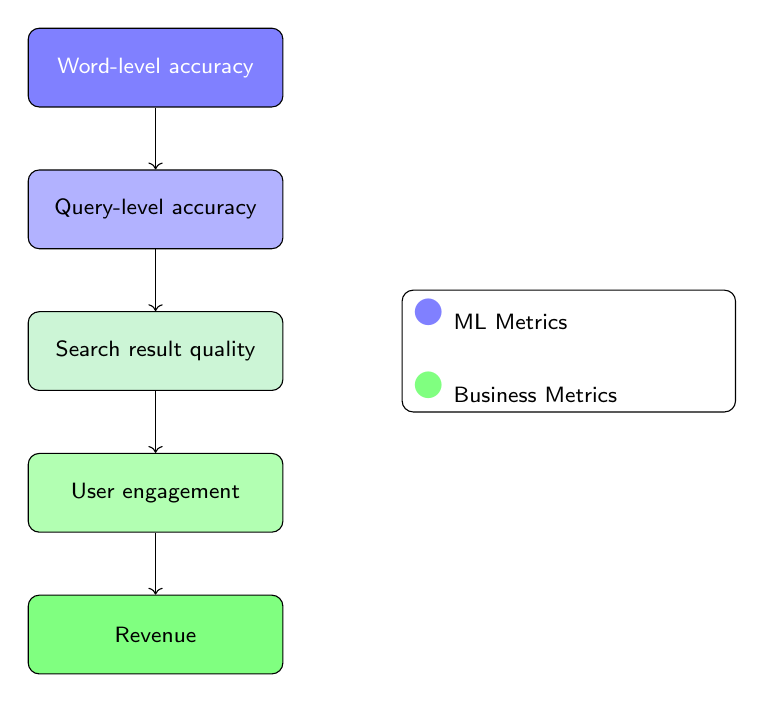
\begin{tikzpicture}[
        node distance=1.8cm,
        align=center,
        font=\footnotesize,
        every node/.style={rounded corners, draw, minimum height=1cm, text width=3cm, align=center}
    ]
        % Nodes with gradient colors
        \node[fill=blue!50, text=white] (word) {Word-level accuracy};
        \node[below of=word, fill=blue!30, text=black] (query) {Query-level accuracy};
        \node[below of=query, fill=blue!20!green!20, text=black] (search) {Search result quality};
        \node[below of=search, fill=green!30, text=black] (engagement) {User engagement};
        \node[below of=engagement, fill=green!50, text=black] (revenue) {Revenue};

        % Arrows
        \draw[->] (word) -- (query);
        \draw[->] (query) -- (search);
        \draw[->] (search) -- (engagement);
        \draw[->] (engagement) -- (revenue);

        \node[right=1.5cm of search, align=left, text width=4cm] (legend) {
            {\color{blue!50}\Huge $\bullet$} ML Metrics\\[0.5cm]
            {\color{green!50}\Huge $\bullet$} Business Metrics
        };
    \end{tikzpicture}
    \caption{Illustration of finding value metrics: ML metrics (blue) transition into business metrics (green) through intermediate steps, representing a compromise between the technical and business teams.}
    \label{fig:value_metrics}
\end{figure}


\subsection{Ethical Considerations and Societal Value}

As part of assessing the value of a machine learning project, it is essential to evaluate the ethical implications and societal impact of the work. Beyond just financial returns or technical feasibility, every project should be scrutinized for its potential to create net positive societal value. If a project does not contribute meaningfully to society, it may not be worth pursuing, regardless of its economic viability. \newline

Ethical considerations vary widely by domain, whether in healthcare, finance, or online retail. These considerations include fairness, potential biases, and the broader implications of deploying the technology. For instance, ensuring that a loan approval algorithm is free from discriminatory bias is critical in finance, just as maintaining equitable access to care is essential in healthcare applications. It is highly recommended to consult ethical frameworks specific to your industry to guide these evaluations. \newline

Raising ethical concerns and openly debating them within the team can lead to more informed and thoughtful decisions. If there are doubts about whether a project will truly benefit humanity or align with societal values, discussing these issues collaboratively often helps teams reach a better consensus. As a result, some projects that might seem economically sound on the surface may still be deprioritized if they fail to contribute positively to people's lives. \newline

Ultimately, machine learning practitioners should strive to focus their efforts on projects that move humanity forward. By dedicating resources to initiatives that both align with ethical principles and create tangible societal benefits, teams can ensure their work contributes meaningfully to the world. Prioritizing these aspects helps build not only impactful solutions but also a sense of purpose within the project team. \newline


\section{Milestones and Resourcing}

Once a problem has been identified, a solution proposed, and due diligence completed to confirm the project's feasibility and value, the final steps of the scoping process involve determining milestones and resourcing. These steps ensure that the project is well-defined and has a clear roadmap for execution.

\subsection{Milestones}

Determining milestones involves specifying the key objectives and metrics that define the project's success. For machine learning projects, these typically include:
\begin{itemize}
    \item \textbf{Machine learning metrics:} Metrics such as accuracy, precision-recall, or other performance indicators relevant to the problem.
    \item \textbf{Fairness metrics:} For applications requiring equitable outcomes, metrics to assess bias or fairness may also be specified.
    \item \textbf{Software metrics:} Specifications for system performance, such as latency, throughput, or queries per second, given the computational resources available.
    \item \textbf{Business metrics:} Estimates of the business impact, such as incremental revenue or user engagement improvements, if such calculations are feasible.
\end{itemize}

If defining these specifications proves challenging, a benchmarking exercise or a proof of concept (POC) can be conducted. A POC helps test the feasibility of certain metrics, such as accuracy or latency, and provides valuable insights to refine milestones and better define the project's scope.

\subsection{Resourcing}

Resourcing focuses on identifying and securing the necessary inputs to achieve the milestones within a specified timeline. Key aspects of resourcing include:
\begin{itemize}
    \item \textbf{Data:} How much data is required, and from which sources or teams will it be obtained?
    \item \textbf{Personnel:} What expertise is needed, and which team members or cross-functional teams will contribute?
    \item \textbf{Support:} What software integrations, infrastructure, or assistance from external teams, such as data engineering or IT, are required?
    \item \textbf{Timeline:} A realistic schedule with defined deliverables and deadlines for achieving milestones.
\end{itemize}

A clear understanding of resourcing needs not only ensures that the project is achievable but also helps in aligning expectations with stakeholders. In cases where resource requirements are unclear, benchmarking similar projects or completing a POC can provide clarity. This allows teams to more confidently allocate resources and plan for the larger-scale execution of the project. \newline

In summary, milestones and resourcing are essential to define the scope and plan for the successful execution of machine learning projects. These steps transform ideas into actionable plans, aligning technical and business objectives to achieve meaningful results.




\part{Data}


\chapter{Collecting Data}

Collecting data with machine learning in mind is not just about quantity—it's about collecting the \textbf{right} data, in the \textbf{right} way. While many projects begin with existing data collected for other purposes, designing your own data collection strategy gives you a strategic advantage: you control what your model will learn, and what it can’t.
\newline

This chapter provides practical guidelines for designing data collection processes that produce machine learning–ready datasets.

\textbf{Key points:}
\begin{itemize}
    \item Define the modeling goal before collecting data
    \item Ensure the data reflects real-world deployment conditions
    \item Label Consistency
    \item Capture sufficient diversity (but avoid redundancy)
    \item Anticipate failure cases and edge conditions
    \item Avoid hidden leakage through metadata or proxies
\end{itemize}


\section{Define the Modeling Goal Before Collecting Data}

Before collecting anything, define what the model is supposed to do—and how success will be measured. Vague goals like “predict something useful” lead to data that's too broad, too noisy, or irrelevant for modeling.
\newline

Clarify the task type (classification, regression, ranking, etc.), the target variable, and the real-world constraints. Ask: What inputs will be available at inference time? What predictions need to be made? What does a good prediction look like?
\newline

This decision impacts everything—from which data you collect, to how it’s labeled, to which edge cases need special attention. Collecting without a defined modeling goal is like building a bridge without knowing the river width.
\newline

If multiple goals are possible, focus on the one with the highest potential value and the clearest decision boundary. You can collect auxiliary data later, but your initial dataset should be optimized for a specific use case.

\begin{examplebox}
A logistics company wanted to “predict delivery problems,” so they collected sensor and driver data without defining what a “problem” meant. After months of data collection, they realized different departments had different interpretations—delays, customer complaints, or damaged goods. None of the labels aligned, and the dataset couldn’t support any reliable model.
\end{examplebox}



\section{Ensure the Data Reflects Real-World Deployment Conditions}

Data collected under ideal, artificial, or controlled conditions often fails in the real world. Your training data must resemble the data the model will see at inference time—not what’s easy to collect.

This includes the same input modalities, noise levels, device types, user behavior, and context. If the model will be deployed on mobile devices, don’t train it solely on clean desktop data. If inference happens with missing or delayed inputs, simulate that during collection.

Also consider **temporal drift**—data collected today may not represent future conditions. In such cases, design continuous data collection pipelines and plan for regular model retraining.

If your training data is "too clean" or doesn't reflect deployment variability, your model will learn unrealistic patterns and break when exposed to the real world.

\begin{examplebox}
A fraud detection system trained on historic bank data failed after deployment because customer behavior changed post-pandemic. The model had never seen mobile payments or digital wallets in training. Including recent, real-world samples in the initial data collection would have made the system more robust.
\end{examplebox}



\section{Label Consistency}

Data quality plays a crucial role in machine learning projects, and ensuring consistent labeling is one of the most important aspects of dataset preparation. Inconsistent labeling can lead to confusion for the learning algorithm and significantly impact model performance. This section explores why defining data consistently is challenging and how inconsistencies arise even when labelers are diligent and well-intentioned. \newline

To illustrate the problem, consider the example of iguana detection (Figure~\ref{fig:iguana_ambiguous_labeling}). Suppose you collect hundreds of images of iguanas and send them to labelers with the instruction: \textit{Use bounding boxes to indicate the position of iguanas.} Even with the same instruction, different labelers may interpret the task differently:
\begin{itemize}
    \item One labeler may mark each iguana separately with tight bounding boxes around their bodies.
    \item Another may include the tail, creating larger bounding boxes that overlap.
    \item A third labeler might take an entirely different approach, drawing a single bounding box covering all iguanas in the image.
\end{itemize}
Each of these approaches could be reasonable on their own, but if different labelers follow different conventions within the same dataset, the learning algorithm will struggle to generalize, leading to suboptimal model performance.

\begin{figure}[H]
    \centering
    \includegraphics[width=0.8\textwidth]{data_figures/iguana_ambiguous_labeling.png}
    \caption{Different interpretations of bounding box labeling for iguanas. Some labelers tightly enclose each iguana individually, others include the full tail, and some use a single bounding box for the entire group. Inconsistent labeling conventions like these can lead to confusion for the learning algorithm.}
    \label{fig:iguana_ambiguous_labeling}
\end{figure}

This issue is not limited to iguana detection but is prevalent in real-world computer vision applications, such as phone defect detection (Figure~\ref{fig:phone_ambiguous_labeling}). Consider a dataset where labelers annotate defects on smartphone screens. The following inconsistencies may arise:
\begin{itemize}
    \item One labeler may mark only the most prominent scratch.
    \item Another might highlight both the scratch and smaller defects like pits or dents.
    \item A third may draw a large bounding box encompassing the entire defective area.
\end{itemize}
If different labelers use different conventions, the dataset becomes ambiguous, making it difficult for the model to learn effectively.

\begin{figure}[H]
    \centering
    \includegraphics[width=0.8\textwidth]{data_figures/phone_ambiguous_labeling.png}
    \caption{Variations in defect labeling on smartphone screens. One labeler marks only the most prominent scratch, another includes smaller defects like pits, while a third uses a large bounding box covering the entire defective area. Ensuring a consistent labeling strategy helps improve model training and accuracy.}
    \label{fig:phone_ambiguous_labeling}
\end{figure}

The key takeaway is that defining clear and consistent labeling guidelines is critical for creating high-quality training data. When labelers follow the same conventions, models are more likely to learn the right patterns. In the following sections, we will explore best practices for defining and organizing data, ensuring consistency in labeling, and improving the overall quality of datasets to set up machine learning models for success.

\subsection{Label Consistency Across Different Types of Data}

A useful framework for understanding label consistency challenges in machine learning is based on two key factors:
\begin{itemize}
    \item Whether the data is \textbf{unstructured} (e.g., images, text, audio) or \textbf{structured} (e.g., numerical or categorical tabular data).
    \item Whether the dataset is \textbf{small} (fewer than 10,000 examples) or \textbf{large} (greater than 10,000 examples).
\end{itemize}

This categorization highlights how best practices for ensuring label consistency differ depending on the nature and scale of the dataset. The following table provides an overview of these distinctions:

\begin{table}[H]
    \centering
    \renewcommand{\arraystretch}{1.5}
    \begin{tabular}{|p{3.5cm}|p{5.5cm}|p{5.5cm}|}
        \hline
        \textbf{} & \textbf{Unstructured Data} & \textbf{Structured Data} \\
        \hline
        \textbf{Small Data} & Manufacturing visual inspection with 100 images. Clean labels are critical.  & Housing price prediction with 50 examples. Clean labels are critical. \\
        \hline
        \textbf{Large Data} & Speech recognition with 50 million samples. Humans can label data, data augmentation is helpful. & Online shopping recommendations for 1 million users. Emphasis on data process, harder to obtain more data. \\
        \hline
    \end{tabular}
    \caption{Labeling challenges for different types and sizes of datasets.}
    \label{tab:label_consistency_framework}
\end{table}

We can now examine each of these four quadrants individually to understand the unique challenges and best practices for label consistency.

\subsubsection{Unstructured Data – Small Datasets}
For small datasets containing unstructured data, such as images in a manufacturing inspection task, clean labels are essential. With only a few hundred training examples, each mislabeled instance represents a significant portion of the dataset. Since the dataset is small enough for human review, manual label correction is a viable strategy to ensure consistency. Annotators should align on a clear labeling standard early on to avoid inconsistencies that might degrade model performance.

\subsubsection{Unstructured Data – Large Datasets}
For large unstructured datasets, such as speech recognition with millions of training examples, manual review of every sample is infeasible. However, human labelers can still be used to annotate data, and data augmentation techniques can help synthesize additional labeled examples. Ensuring consistency in large datasets requires well-documented labeling guidelines and automated quality control processes to detect labeling errors and inconsistencies at scale.

\subsubsection{Structured Data – Small Datasets}
In structured data problems with small datasets, such as predicting housing prices based on features from a few dozen properties, label consistency is equally important. Since there are relatively few training examples, each data point carries a high weight in determining model performance. Careful curation and validation of structured attributes, such as ensuring uniformity in feature definitions (e.g., how square footage is recorded), can help maintain consistency.

\subsubsection{Structured Data – Large Datasets}
For structured data with large datasets, such as online shopping recommendations for millions of users, the emphasis shifts from manual label correction to data process design. With a dataset this large, it is impractical for human annotators to verify each label. Instead, organizations must implement well-defined data pipelines, ensuring that attributes such as user preferences and item metadata are processed and stored consistently. Unlike unstructured data, data augmentation is rarely feasible for structured problems, making high-quality data collection and processing even more critical.

Understanding where a given machine learning problem falls within this framework can help practitioners develop appropriate strategies for label consistency, whether through manual correction, automation, or improved data collection processes.


\subsection{The Importance of Label Consistency in Small and Large Datasets}

Label consistency is especially critical when working with small datasets. In such cases, even minor inconsistencies in labeling can significantly impact model performance. Conversely, in large datasets, while label consistency remains important, the model may be able to generalize better if sufficient data is available. However, rare events within large datasets often pose similar challenges to small data problems. Figure~\ref{fig:small_data_label_consistency_importance} illustrates these differences.

\begin{figure}[H]
    \centering
    \includegraphics[width=0.9\textwidth]{data_figures/small_data_label_consistency_importance.png}
    \caption{Impact of label consistency on small and large datasets. Noisy labels in small datasets make it difficult to fit a reliable function, whereas with more data, the model can generalize better despite noise. However, clean labels significantly improve performance even in small datasets.}
    \label{fig:small_data_label_consistency_importance}
\end{figure}

\subsubsection{Small Datasets: Why Clean Labels Matter}
Consider a scenario where we want to predict the speed of a motor rotor based on input voltage. If we only have five training examples, label noise can make it extremely difficult to determine the correct function mapping voltage to speed. The uncertainty in the data makes it hard to decide whether the relationship should be linear, non-linear, or have plateaus. \newline

However, if the same small dataset had clean and consistent labels, the learning algorithm could confidently fit a function, even with only a few examples. This highlights why, in small datasets, label consistency is often more important than simply increasing dataset size.

\subsubsection{Large Datasets: Averaging Over Noisy Labels}
In contrast, when working with a large dataset (e.g., speech recognition with millions of examples), label noise is less problematic because the model can average over noisy samples. With enough data, a well-structured model can still learn a reliable pattern despite some level of label noise. However, ensuring label consistency across a large dataset remains beneficial, as large datasets often contain subdomains where data is sparse.

\subsubsection{Rare Events in Large Datasets: A Small Data Challenge}
Even in large datasets, small data challenges exist in the form of rare events. For example:
\begin{itemize}
    \item In self-driving car datasets, the total dataset may be vast, but rare occurrences (e.g., a child running across a highway) have very few labeled instances.
    \item In web search engines, most search queries occur frequently, but some rare queries have very little data available for training.
    \item In product recommendation systems, while large e-commerce platforms have millions of products, some items have very few purchases, making recommendations difficult.
\end{itemize}

In such cases, ensuring label consistency for rare events is just as important as for small datasets. If a model encounters inconsistent labeling for rare but critical events, its ability to make reliable predictions suffers. \newline

Ultimately, label consistency is crucial across all dataset sizes. For small datasets, it allows learning algorithms to make accurate predictions with fewer examples. For large datasets, it ensures that rare events, which often carry high importance, are handled correctly.

\subsection{Improving Label Consistency}

Ensuring label consistency is an iterative process that involves refining labeling guidelines, standardizing definitions, and sometimes even modifying the dataset itself. Below, we outline several best practices to systematically improve label consistency in machine learning projects.

\subsubsection{Iterative Label Review and Agreement}
A simple but effective approach to identifying inconsistencies is to have multiple labelers annotate the same set of examples. If significant disagreements arise:
\begin{itemize}
    \item Organize discussions between labelers, subject matter experts, and engineers to agree on a standardized labeling convention.
    \item Document these agreed-upon guidelines to ensure uniformity across future labels.
    \item In some cases, have labelers annotate the same data at different times to check if their own labels remain consistent.
\end{itemize}

If labelers find that input features (X) are insufficient to make confident labeling decisions, consider modifying the data collection process. For example, if phone images are too dark to assess scratches accurately, improving lighting conditions during image capture can enhance labeling consistency.

\subsubsection{Merging Classes to Reduce Ambiguity}
When labelers struggle to distinguish between similar categories—such as differentiating between "deep scratches" and "shallow scratches" on a phone—ambiguities can lead to inconsistent labels. In such cases, merging similar categories into a single class (e.g., “scratches”) can simplify the labeling task and reduce errors. While some use cases may require precise differentiation, removing unnecessary class distinctions can often enhance model performance.

\subsubsection{Introducing a Borderline or Uncertainty Class}
For genuinely ambiguous cases, adding an explicit "borderline" class can improve label consistency. For example:
\begin{itemize}
    \item In phone defect detection, rather than forcing labelers to classify uncertain scratches as either “defect” or “not a defect,” introducing a "borderline defect" category can reduce inconsistencies.
    \item In speech recognition, when an audio clip is unintelligible, instead of labelers guessing, an “unintelligible” tag can provide a more standardized way of handling unclear cases.
\end{itemize}

This strategy helps models learn clearer distinctions between well-defined categories while maintaining a structured way to handle ambiguous cases.

\subsubsection{Scaling Label Consistency for Large Datasets}
For small datasets, inconsistencies can often be resolved through direct discussions among a small team of labelers. However, large datasets require a more scalable approach:
\begin{itemize}
    \item Establish a small core team to define precise labeling guidelines before expanding to a larger group of annotators.
    \item Provide detailed instructions and regular calibration checks to maintain consistency across a large labeling workforce.
    \item Instead of relying heavily on consensus voting (which is sometimes overused), prioritize refining label definitions to minimize disagreements in the first place.
\end{itemize}

\subsubsection{Towards Better Labeling Tools and Automation}
Currently, many teams rely on manual processes to refine label consistency, but there is a growing need for better machine learning tools to:
\begin{itemize}
    \item Detect inconsistent labels automatically.
    \item Facilitate iterative refinement of label definitions.
    \item Streamline the relabeling process with minimal human intervention.
\end{itemize}

While these tools are still emerging, improving label consistency through systematic human-driven processes remains one of the most effective ways to enhance dataset quality. These principles, combined with structured discussions and well-defined labeling conventions, can significantly improve the accuracy and reliability of machine learning models.



\section{Capture Sufficient Diversity (but Avoid Redundancy)}

A model can only generalize to what it has seen. If the training data lacks diversity, the model will underperform in edge cases or new environments. Diversity should be intentional: include different classes, conditions, users, devices, times of day, geographic regions, or other relevant dimensions.

However, collecting more data is not always better. Redundant data—highly similar or repeated samples—adds cost without adding information. Worse, it can skew the learning process and bias the model toward frequent or easy patterns.

Aim for \textbf{informative coverage}, not brute-force scale. Identify key axes of variation, then ensure your dataset spans them. Stratified sampling can help here. Keep track of where the data came from and how it was selected—metadata matters.

\begin{examplebox}
In a wildlife image classification task, over 80\% of the training photos came from just two camera traps. As a result, the model learned background cues (e.g., vegetation type, lighting) instead of animal features. When tested on new locations, accuracy collapsed. Sampling from more diverse environments fixed the issue.
\end{examplebox}



\section{Anticipate Failure Cases and Edge Conditions}

Most models don't fail on the average case—they fail on edge cases. These might be rare classes, atypical input combinations, low-quality samples, or ambiguous scenarios. If these aren't represented in the training data, the model will fail silently when it encounters them.

Think ahead: Where could the model break in deployment? What inputs are rare but high-impact? What’s the worst-case scenario for incorrect predictions? Proactively collecting such examples improves robustness and helps define safe operating boundaries.

You don’t need large amounts of edge-case data—just enough to test performance and possibly adjust decision thresholds or fallback behavior.

\textbf{Tip:} When collecting data, don’t just maximize coverage—stress-test it.

\begin{examplebox}
In a facial recognition system, most of the collected images were well-lit, frontal shots. But real-world use included low light, occlusions, and extreme angles. Without these edge cases in the training set, the system failed frequently in the field—especially in security-critical scenarios.
\end{examplebox}




\chapter{EDA for Structured Data}

Exploratory Data Analysis (EDA) is a crucial step in any machine learning 
project. It helps in understanding the dataset, identifying patterns, and 
detecting potential issues before modeling. \newline

EDA is purely \textbf{observational}—it does not involve modifying, fixing, 
or cleaning the data. Instead, it provides a clear picture of the dataset 
as it exists, allowing us to assess its structure, distributions, and 
inconsistencies. This is particularly important because the dataset’s 
history—how it was collected, processed, or formatted—was not necessarily 
under our control. \newline

Since EDA is about discovering what is already there, it should be performed 
at the very beginning, using the initial dataset in its raw form. Once we 
observe and understand the data, any modifications, transformations, or 
cleaning steps that follow are entirely under our control. While EDA can be 
repeated after changes, it is no longer required in the same way—once the 
data has been analyzed and adjusted, its behavior is known. \newline

This chapter focuses on \textbf{structured data}—data organized in tabular 
form, where each row represents an observation and each column has a 
\textit{human-understandable} meaning, such as \texttt{age}, \texttt{height}, 
or \texttt{income}. This is in contrast to unstructured data like images, 
audio, or free text, where columns may represent pixel intensities, 
waveform amplitudes, or token embeddings, and are not directly interpretable 
on their own. \newline

EDA for unstructured data is also possible and equally important, but it 
requires fundamentally different techniques and tools. Due to these 
differences, unstructured data will be addressed separately in a dedicated 
chapter. \newline

A systematic EDA approach ensures a thorough analysis while avoiding 
unnecessary detours. By systematically exploring the dataset, we gain the 
insights needed to make informed preprocessing and modeling decisions.
\newline


\textbf{Key points:}
\begin{itemize}
    \item Variable distributions
    \item Outliers, anomalies, and missing values
    \item Comparing variables
    \item Dimensionality reduction
    \item Pattern discovery
\end{itemize}

\textbf{Variable distributions}: Understanding the distribution of each variable is the first step in EDA. This involves assessing \textbf{central tendency} (mean, median, mode) and \textbf{dispersion} (standard deviation, variance, interquartile range). For \textbf{continuous variables}, histograms provide a clear visualization of the distribution shape, revealing skewness, multimodal distributions, or extreme values. Q-Q plots can help assess deviations from normality. For \textbf{categorical variables}, frequency tables and bar charts summarize the distribution, highlighting dominant categories and potential imbalances in the dataset.
\newline

\textbf{Outliers, anomalies, and missing values}: Outliers and anomalies can signal potential data quality issues or uncover meaningful insights. Anomalies include impossible values (e.g., an apartment listed on the seventh floor when the building has only five) or unusual but plausible occurrences that warrant further investigation. Missing values, whether systematic or random, should be analyzed to determine their impact and whether imputation, removal, or domain-specific handling is necessary.
\newline

\textbf{Comparing variables}: Examining relationships between variables provides insights into dependencies and correlations. Correlation analysis measures linear relationships between numerical variables, scatter plots visualize pairwise relationships, and cross-tabulations help analyze categorical variables.
\newline

\textbf{Dimensionality reduction}: When working with high-dimensional data, techniques like Principal Component Analysis (PCA) and t-SNE help uncover hidden structures and simplify modeling.
\newline

\textbf{Pattern discovery}: Identifying patterns in data helps uncover structure, trends, and hidden relationships that may not be immediately obvious. Clustering techniques, such as K-means and hierarchical clustering, group similar observations together, revealing natural subgroups. Other approaches, such as association rule mining (e.g., Apriori algorithm) for categorical data or time-series decomposition for sequential data, can help detect meaningful patterns beyond clustering.
\newline


\section{Variable Distributions}

Assessing the distribution of each variable is a fundamental step in exploratory data analysis. It provides insights into the data's range, central tendency, dispersion, and overall shape. By thoroughly understanding the distribution of each variable, we can detect data quality issues, recognize patterns, and inform downstream modeling decisions.

\subsection{Understanding Central Tendency and Dispersion}

Two key characteristics define a variable’s distribution:  
- \textbf{Central tendency}: Measures of central tendency describe where most of the data points lie. Common metrics include:
  \begin{itemize}
      \item \textbf{Mean}: The arithmetic average of the values.
      \item \textbf{Median}: The middle value when the data is sorted.
      \item \textbf{Mode}: The most frequently occurring value(s).
  \end{itemize}
- \textbf{Dispersion}: Measures of dispersion describe the spread of data points. Key metrics include:
  \begin{itemize}
      \item \textbf{Standard deviation} and \textbf{variance}: Indicate how much values deviate from the mean.
      \item \textbf{Interquartile range (IQR)}: The range between the 25th and 75th percentiles, offering a robust measure of spread.
      \item \textbf{Range}: The difference between the maximum and minimum values.
  \end{itemize}

\subsection{Visualization Techniques for Variable Distributions}

Visualizing variable distributions helps detect patterns, skewness, and anomalies. The choice of visualization depends on the type of variable:

\begin{table}[h]
    \centering
    \begin{tabular}{|l|l|}
        \hline
        \textbf{Variable Type} & \textbf{Recommended Visualization} \\
        \hline
        Numerical (continuous) & Histogram, Q-Q Plot \\
        Categorical & Frequency Table, Bar Chart \\
        \hline
    \end{tabular}
    \caption{Visualization techniques for assessing variable distributions.}
    \label{tab:viz_variable_distributions}
\end{table}

\subsection{Histograms: Examining Continuous Variable Distributions}

Histograms are one of the most effective tools for understanding the distribution of continuous variables. They group data into bins and display the frequency of occurrences, helping answer questions such as:
- Does the variable follow a normal, skewed, or multimodal distribution?
- Are there extreme values or gaps in the distribution?
- Does the data exhibit a uniform spread or strong clustering?

Key considerations when interpreting histograms:
- A \textbf{symmetric bell shape} suggests a normal distribution.
- A \textbf{right-skewed} distribution has a long right tail, indicating potential outliers or a need for transformation.
- A \textbf{left-skewed} distribution has a long left tail, often requiring similar treatment.
- A \textbf{multimodal distribution} (multiple peaks) may indicate the presence of different subpopulations.

For skewed distributions, log-transforming the data before visualization can sometimes improve interpretability.

\subsection{Q-Q Plots: Assessing Normality}

A quantile-quantile (Q-Q) plot compares the quantiles of a variable’s distribution to the quantiles of a theoretical normal distribution. It helps assess whether the data is normally distributed:
- If points fall along a straight diagonal line, the distribution is approximately normal.
- Curvature at the ends suggests skewness.
- Deviations from the line indicate a non-normal distribution, which may affect statistical assumptions in modeling.

\subsection{Assessing Categorical Variables with Frequency Tables and Bar Charts}

For categorical variables, frequency tables and bar charts provide a clear summary of distribution:
- \textbf{Frequency tables}: Display counts or proportions for each category, highlighting dominant and underrepresented groups.
- \textbf{Bar charts}: Offer a visual representation of category frequencies, making comparisons intuitive.

Key aspects to look for:
- A \textbf{highly imbalanced distribution} (one category dominating) might require resampling techniques or a different modeling approach.
- Unexpected categories or typos may indicate data quality issues.
- The presence of too many unique categories (high cardinality) might necessitate grouping similar values.


\subsection{Key Takeaways}

Understanding the distribution of each variable individually is a critical first step in EDA. By summarizing central tendency, dispersion, and shape—supported by histograms, Q-Q plots, and bar charts—we can:
- Detect potential data quality issues.
- Decide whether transformations are necessary.
- Prepare for further analysis, such as outlier detection and variable comparisons.

A well-executed variable distribution analysis lays the foundation for deeper insights in subsequent EDA steps.



\section{Outliers, Data Errors, and Missing Values}

Detecting outliers, data errors, and missing values is a critical step in 
exploratory data analysis (EDA). These elements can indicate errors, 
inconsistencies, or rare patterns that warrant further investigation. 
This section focuses on practical methods to identify and visualize them 
effectively.

\subsection{Outliers: Detecting Extreme Values}

Outliers are data points that deviate significantly from the overall 
distribution. They can result from measurement errors, data entry 
mistakes, or genuinely rare events. Identifying outliers is crucial, 
as they can distort statistical summaries and impact model performance.
\newline

Outlier detection depends on the type of variable:  
\newline
- For \textbf{nominal and ordinal variables}, the only meaningful way to detect 
  outliers is by analyzing rare categories.  
\newline
- For \textbf{metric variables (interval or ratio scale)}, both visualization and 
  statistical methods can be used to identify extreme values.
\newline

\subsubsection{Outliers in Nominal and Ordinal Variables}

Since nominal and ordinal variables represent \textbf{categories}, outlier detection 
is based on \textbf{frequency distributions}. Categories that appear very rarely in 
the dataset can be considered potential outliers.
\newline

\textbf{Method:}  
\newline
- Count occurrences of each category.  
- Identify categories that occur significantly less frequently than others.  
- Visualize the distribution using \textit{bar charts}, where rare categories 
  appear with noticeably smaller bars.
\newline

\textbf{Interpretation:}  
\newline
- Rare categories may indicate unusual data points, potential misclassifications, 
  or errors in data collection.  
- In some cases, rare categories are valid but require further domain knowledge 
  to assess their significance.  
\newline

\subsubsection{Outliers in Metric Variables (Interval or Ratio Scale)}

For numerical variables, outliers can be detected through \textbf{visualization} 
and \textbf{statistical techniques}.
\newline

\paragraph{Visualizing Outliers}
Before applying formal statistical methods, visualizations provide an intuitive 
overview of extreme values:
\newline
- \textit{Box Plots}: Display data distribution and highlight outliers as 
  points beyond whiskers.
\newline
- \textit{Scatter Plots}: Help detect outliers by showing unusual values in 
  relation to other variables.
\newline
- \textit{Z-Score Plot}: Standardizes data to highlight extreme deviations 
  from the mean.
\newline

\paragraph{Statistical Methods for Outlier Detection}
To systematically identify outliers, the following approaches are commonly used:
\newline
- \textit{Interquartile Range (IQR) Method}:  
  - Compute the first (Q1) and third (Q3) quartiles.  
  - Define outliers as values beyond 1.5 times the IQR from the quartiles.  
\newline
- \textit{Z-Score Method}:  
  - Standardize data and identify values with Z-scores exceeding a threshold 
    (commonly \( |Z| > 3 \)).  
\newline
- \textit{Formal Outlier Tests}:  
  - Statistical tests such as distribution-based outlier detection or 
    anomaly detection models can be used to flag extreme values.
\newline

\textbf{Interpretation:}  
\newline
- Some extreme values may be valid observations rather than errors.  
- Decisions on handling outliers depend on domain knowledge and the specific 
  impact of outliers on the analysis.  
\newline


\subsection{Data Errors: Finding Implausible or Impossible Values}

Data errors are unexpected data points given domain knowledge or internal inconsistencies. Unlike outliers, which may be valid, data errors can indicate incorrect or inconsistent information.
\newline

Common ways to detect anomalies:
\newline

\textbf{Logical Checks:}
- Identify impossible values (e.g., negative age, invalid heights).
- Detect inconsistencies (e.g., a deceased person with transactions).
\newline

\textbf{Cross-Feature Validation:}
- Verify expected relationships (e.g., fuel efficiency vs. weight).
- Check for duplicated records where uniqueness is required.
\newline

\textbf{Visualizations:}
- \textit{Scatter Plots}: Identify deviations from expected trends.
- \textit{Pair Plots}: Detect anomalies across multiple variables.
- \textit{Heatmaps}: Identify inconsistent variable relationships.
\newline

\textbf{One-Hot Encoding Validity:}

Ensure that each instance has at least one active category. A row with all zeros in a one-hot encoded variable set is often an error. This can be seen as a hidden missing value, because all values exist, but the categorical information is still absent.

\begin{examplebox}
A dataset categorizes customer membership as \texttt{Basic}, \texttt{Premium}, or \texttt{VIP}, using one-hot encoding. A row where all three columns are zero suggests missing or incorrect data since every customer should belong to one category.
\end{examplebox}


\subsection{Missing Values: Identifying Data Gaps}

Missing values occur due to data entry errors, omitted responses, or sensor failures. 
Detecting them is crucial for ensuring data integrity before analysis.
\newline

\textbf{Summary Statistics:}  
\newline
- Count missing values per variable.  
- Compute missing percentages to assess their impact.  
\newline

\textbf{Visualizations:}  
\newline
- \textit{Bar Plots}: Show the percentage of missing values per variable.  
- \textit{Heatmaps}: Highlight missingness patterns across the dataset.  
\newline


\section{Comparing Variables}

Examining relationships between variables is essential for understanding dependencies, correlations, and potential interactions. This step helps detect redundant features, uncover predictive relationships, and guide feature engineering decisions. 

\subsection{Numerical Metrics for Variable Comparison}

Before visualizing relationships, computing numerical summaries can provide an initial sense of correlation and dependency between variables.
\newline

\textbf{Correlation Analysis:}
- Pearson correlation: Measures linear relationships between numerical variables.
- Spearman correlation: Captures monotonic relationships, useful for ranked data.
- Kendall’s Tau: Suitable for ordinal variables or small sample sizes.
\newline

\textbf{Covariance:}
- Measures the directional relationship between two variables but does not standardize values, making it sensitive to scale.
\newline

\textbf{Contingency Tables:}
- Summarize relationships between two categorical variables by counting occurrences of each combination.
- Used to compute metrics like chi-square tests for independence.
\newline

\textbf{Tools for Numerical Comparison:}
- In Python: \texttt{pandas.DataFrame.corr()}, \texttt{scipy.stats.spearmanr()}.
- In R: \texttt{cor()}, \texttt{cor.test()}, \texttt{chisq.test()}.

\subsection{Visualizing Relationships Between Numerical Variables}

\textbf{Scatter Plots:}
- The most direct way to visualize relationships between two numerical variables.
- Patterns may reveal correlations, clusters, or non-linear trends.
- Use color coding to introduce a third categorical variable.
\newline

\textbf{Pair Plots (Scatterplot Matrices):}
- A compact way to visualize multiple pairwise relationships in a dataset.
- Useful for detecting redundant features.
\newline

\textbf{Heatmaps of Correlation Matrices:}
- Display correlations between all numerical features.
- Highlight strong positive or negative relationships.
\newline

\textbf{Hexbin and Density Plots:}
- For large datasets, hexbin plots group scatter points into hexagonal bins, revealing density patterns.
- Kernel density estimation (KDE) plots help visualize probability distributions between two variables.
\newline

\subsection{Analyzing Relationships Between Categorical Variables}

\textbf{Grouped Bar Charts:}
- Compare distributions of one categorical variable across levels of another.
- Useful for detecting category imbalances.
\newline

\textbf{Mosaic Plots:}
- Show proportions of categorical variables in a hierarchical manner.
- Useful for visualizing dependencies between categorical features.
\newline

\textbf{Stacked or Side-by-Side Bar Charts:}
- Compare category distributions across groups.
- Helps understand relative proportions in each category.
\newline

\textbf{Chi-Square Tests for Independence:}
- Assess whether two categorical variables are significantly related.
- Applied to contingency tables to determine statistical dependence.
\newline

\textbf{Tools for Categorical Analysis:}
- In Python: \texttt{seaborn.catplot()}, \texttt{stats.chi2\_contingency()}.
- In R: \texttt{ggplot2::geom\_bar()}, \texttt{MASS::mosaicplot()}.
\newline

\subsection{Comparing Numerical and Categorical Variables}

\textbf{Box Plots:}
- Show how a numerical variable varies across categories.
- Useful for identifying category-based differences in distributions.
\newline

\textbf{Violin Plots:}
- Combine box plots and density plots to show distribution shape.
- Particularly useful for detecting bimodal distributions within categories.
\newline

\textbf{ANOVA and Kruskal-Wallis Tests:}
- Assess whether a numerical variable differs significantly across categories.
- ANOVA assumes normality, while Kruskal-Wallis is non-parametric.
\newline

\subsection{Mutual Information for Dependency Detection}

Mutual information (MI) is a powerful metric that quantifies the dependency between two variables, capturing both linear and non-linear relationships. Unlike correlation coefficients, which are limited to linear (Pearson) or monotonic (Spearman, Kendall) associations, mutual information detects any kind of statistical dependency.
\newline

\textbf{Definition:}
Mutual information between two random variables \( X \) and \( Y \) is given by:

\[
I(X; Y) = \sum_{x \in X} \sum_{y \in Y} P(x, y) \log \frac{P(x, y)}{P(x) P(y)}
\]

where \( P(x, y) \) is the joint probability distribution, and \( P(x) \) and \( P(y) \) are the marginal distributions of \( X \) and \( Y \). High mutual information indicates strong dependency, while zero mutual information implies independence.
\newline

\textbf{Advantages of Mutual Information:}
- Detects both linear and non-linear relationships.
- Works for numerical and categorical variables.
- Handles cases where traditional correlation metrics fail (e.g., periodic relationships).
\newline

\textbf{Limitations:}
- Does not distinguish between positive and negative associations.
- Requires proper estimation of probability distributions, which may be sensitive to binning in discrete cases.
\newline




\section{Dimensionality Reduction}

When exploring high-dimensional datasets, it can be challenging to understand relationships between variables or detect meaningful structures. \textbf{Dimensionality reduction} techniques help visualize and summarize complex datasets by reducing the number of features while preserving the most relevant information. In the context of EDA, the goal is not to transform features for modeling but to uncover patterns, groupings, and structures in the data.

\subsection{Why Use Dimensionality Reduction in EDA?}

Dimensionality reduction is useful in EDA for:
\begin{itemize}
    \item \textbf{Visualizing high-dimensional data} in 2D or 3D to detect clusters and patterns.
    \item \textbf{Identifying redundant or correlated features} by analyzing variance distribution.
    \item \textbf{Detecting underlying structure} that might not be obvious in raw data.
    \item \textbf{Understanding feature relationships} in a compressed representation.
\end{itemize}

\subsection{Principal Component Analysis (PCA) for Exploration}

\textbf{Principal Component Analysis (PCA)} is a widely used linear technique for summarizing datasets with many numerical variables. It transforms correlated features into \textbf{uncorrelated principal components}, ranked by their contribution to the dataset’s variance.

\textbf{How PCA helps in EDA:}
\begin{itemize}
    \item \textbf{Variance analysis}: The explained variance plot (scree plot) reveals how much information is retained in each component, helping assess the importance of dimensions.
    \item \textbf{Visualizing relationships}: Plotting data in the space of the first two or three principal components allows detection of clusters, separations, and anomalies.
    \item \textbf{Feature correlation}: The PCA loadings indicate which original variables contribute most to each principal component, helping identify redundant or dominant features.
\end{itemize}

\textbf{Interpreting PCA in EDA:}
\begin{itemize}
    \item If the first few components explain most of the variance, the dataset has a lower intrinsic dimensionality.
    \item Strong contributions from specific variables to a component indicate high correlations between features.
    \item Well-separated groups in a PCA plot may suggest distinct subpopulations or clusters in the data.
\end{itemize}

\subsection{t-SNE for Detecting Hidden Structures}

\textbf{t-Distributed Stochastic Neighbor Embedding (t-SNE)} is a non-linear method designed for \textbf{visualizing complex, high-dimensional data} in two or three dimensions. Unlike PCA, it does not preserve global variance but focuses on capturing local relationships.

\textbf{How t-SNE helps in EDA:}
\begin{itemize}
    \item \textbf{Cluster identification}: Groups in the data become visually distinct, revealing natural substructures.
    \item \textbf{Detecting anomalies}: Isolated points may indicate outliers or rare patterns.
    \item \textbf{Understanding feature space}: If data separates meaningfully in t-SNE space, there may be strong patterns in the original feature set.
\end{itemize}

\textbf{Considerations when using t-SNE:}
\begin{itemize}
    \item The \textbf{perplexity parameter} controls how much of the global structure is considered—smaller values focus on local patterns, while larger values balance local and global structure.
    \item Results are \textbf{non-deterministic}, meaning different runs can produce slightly different embeddings.
    \item t-SNE is computationally expensive and best suited for smaller datasets.
\end{itemize}

\subsection{UMAP for Efficient Visualization}

\textbf{Uniform Manifold Approximation and Projection (UMAP)} is an alternative to t-SNE that provides \textbf{similar high-dimensional visualizations but with better preservation of global structure} and greater efficiency.

\textbf{UMAP’s advantages for EDA:}
\begin{itemize}
    \item Faster and scalable to large datasets.
    \item Retains both \textbf{local and global structures} better than t-SNE.
    \item Useful for both cluster detection and general structure analysis.
\end{itemize}

\subsection{Key Takeaways}

Dimensionality reduction in EDA helps explore complex datasets by summarizing feature relationships, detecting clusters, and visualizing structures in a lower-dimensional space.

\begin{itemize}
    \item \textbf{PCA} is useful for understanding variance structure and identifying redundant features.
    \item \textbf{t-SNE} is effective for revealing hidden clusters and patterns in high-dimensional data.
    \item \textbf{UMAP} offers a scalable alternative, preserving both local and global structures.
\end{itemize}




\section{Pattern Discovery}

Pattern discovery in exploratory data analysis aims to uncover hidden structures, trends, and regularities within the dataset. Identifying patterns helps in feature engineering, data preprocessing, and understanding the underlying relationships that could impact modeling decisions.

\subsection{Types of Patterns in Data}

Patterns can manifest in various ways, depending on the nature of the data:
\begin{itemize}
    \item \textbf{Clusters}: Groups of similar data points that may indicate different subpopulations or naturally occurring segments.
    \item \textbf{Trends}: Systematic changes over time, often relevant for time-series data.
    \item \textbf{Associations}: Relationships between categorical variables, often discovered through correlation analysis or association rule mining.
    \item \textbf{Repetitive Structures}: Recurring sequences or periodic patterns, common in time-series and textual data.
\end{itemize}

\subsection{Clustering for Pattern Discovery}

Clustering is one of the most effective techniques for uncovering hidden structures in data. It groups data points based on similarity, revealing natural subgroups that can be used for segmentation, anomaly detection, or exploratory insights.

\subsubsection{Clustering Algorithms}

Several clustering algorithms exist, each with different assumptions and strengths:
\begin{itemize}
    \item \textbf{K-means clustering}: A centroid-based method that partitions data into \( k \) clusters by minimizing within-cluster variance.
    \item \textbf{Hierarchical clustering}: Creates a tree-like structure of nested clusters, allowing different levels of granularity.
    \item \textbf{DBSCAN (Density-Based Spatial Clustering)}: Identifies dense regions of data points while marking outliers separately.
    \item \textbf{Gaussian Mixture Models (GMM)}: A probabilistic approach where each cluster is modeled as a Gaussian distribution.
\end{itemize}

\subsubsection{Evaluating Clustering Results}

Assessing the quality of clustering results is crucial for pattern discovery:
\begin{itemize}
    \item \textbf{Silhouette score}: Measures how well-separated clusters are by comparing within-cluster and between-cluster distances.
    \item \textbf{Elbow method}: Helps determine the optimal number of clusters by analyzing variance explained by different \( k \) values.
    \item \textbf{Visualization}: Techniques like t-SNE and PCA allow for 2D representation of clusters to validate separation.
\end{itemize}

\subsection{Correlation and Association Patterns}

Understanding relationships between variables helps in feature selection and predictive modeling. Patterns can be identified using:
\begin{itemize}
    \item \textbf{Correlation matrices}: Show numerical relationships between continuous variables. Pearson correlation captures linear dependencies, while Spearman correlation accounts for monotonic relationships.
    \item \textbf{Association rule mining}: Identifies frequent itemsets and relationships in categorical data. Apriori and FP-Growth algorithms help detect co-occurrence patterns (e.g., "People who buy X often buy Y").
    \item \textbf{Chi-square tests}: Evaluate dependencies between categorical variables, identifying statistically significant relationships.
\end{itemize}

\subsection{Pattern Discovery in Time-Series Data}

For datasets involving time-dependent variables, specialized techniques help detect patterns over time:
\begin{itemize}
    \item \textbf{Rolling averages and smoothing}: Identify long-term trends by reducing short-term fluctuations.
    \item \textbf{Seasonal decomposition (STL)}: Splits a time series into trend, seasonality, and residual components to analyze periodic behavior.
    \item \textbf{Autocorrelation function (ACF)}: Measures how past values influence future values, highlighting repetitive structures.
    \item \textbf{Anomaly detection}: Identifies unusual deviations in time-series data using moving averages, isolation forests, or statistical thresholds.
\end{itemize}

\subsection{Visualizing Patterns}

Visualization techniques are crucial in pattern discovery, making hidden structures interpretable:
\begin{itemize}
    \item \textbf{Heatmaps}: Display correlation patterns between variables.
    \item \textbf{Scatter plots}: Highlight pairwise relationships, trends, and clusters.
    \item \textbf{t-SNE and UMAP}: Reduce high-dimensional data into 2D or 3D spaces for visualization of complex patterns.
    \item \textbf{Dendrograms}: Used in hierarchical clustering to visualize nested cluster structures.
\end{itemize}

\subsection{Key Takeaways}

Pattern discovery provides valuable insights into data structure and relationships, enabling better feature selection, segmentation, and anomaly detection. By combining clustering techniques, correlation analysis, and time-series methods, hidden patterns can be effectively identified and leveraged for modeling.
\newline

A well-executed pattern discovery process enhances the interpretability of data, ultimately improving the decision-making process in machine learning projects.


\section{Summary}
EDA is not a one-time task but an iterative process. New findings often lead to additional questions and refinements. Continuously revisiting and refining analysis ensures a deeper understanding of the data and better decision-making in subsequent modeling steps.



\chapter{EDA for Unstructured Data}

Unstructured data—such as images, audio, and text—presents unique 
challenges for exploratory data analysis (EDA). Unlike structured datasets 
with clearly labeled variables in tabular form, unstructured data lacks 
directly interpretable columns. Its content must first be transformed 
or represented in a meaningful way before statistical or visual 
exploration becomes possible. \newline

Nonetheless, EDA for unstructured data is just as essential. It helps 
reveal patterns, biases, artifacts, and inconsistencies that could 
impact modeling downstream. Given the diversity and complexity of 
unstructured formats, EDA techniques must be tailored to each domain 
and often rely on intermediate representations, such as embeddings, 
image statistics, or audio features. \newline

This chapter outlines a structured EDA approach for unstructured data 
by focusing on core principles that are broadly applicable across 
modalities.
\newline

\textbf{Key points:}
\begin{itemize}
    \item Understanding raw data characteristics (e.g., shape, format, quality)
    \item Summary statistics from domain-specific features 
    \item Visualizing representative samples
    \item Detecting imbalances, artifacts, and noise
    \item Embedding-based exploration (e.g., PCA, t-SNE on learned features)
\end{itemize}


\section{Understanding Raw Data Characteristics}

Before diving into any complex analysis, begin by understanding what your raw data actually is. For unstructured data, this includes verifying shape, format, consistency, and surface-level quality.
\newline

For image data, examine dimensions, color channels, and file formats (e.g., PNG vs.\ JPEG). Confirm that aspect ratios are consistent or document the variance. For audio, inspect sampling rates, duration distributions, and encoding types (e.g., WAV vs.\ MP3). For text, check for encoding issues (e.g., UTF-8 vs.\ Latin-1), average document length, token distributions, and language consistency.
\newline

Corrupted files, unexpected formats, or inconsistent structure are common issues. These can quietly wreck preprocessing pipelines or distort model training—catch them early.
\newline

You don’t need deep domain knowledge to do this part well, just a methodical check of the basics. Log key statistics and anomalies. If the data comes from multiple sources or time points, compare them separately to detect distribution drift or data collection inconsistencies.

\begin{examplebox}
A medical imaging project revealed that 20\% of X-ray files were grayscale PNGs while the rest were RGB JPEGs. Models trained on the mixed set underperformed until the grayscale images were converted to match the RGB format. The format inconsistency was only caught during this initial inspection step.
\end{examplebox}


\section{Summary Statistics from Domain-Specific Features}

Once basic integrity of the raw data is confirmed, extract summary statistics from domain-relevant features. This step helps quantify core characteristics, detect outliers, and uncover unusual distributions that could bias your model.
\newline

For images, compute pixel intensity histograms, brightness, contrast, or edge density. These statistics can expose systematic differences across data sources or timepoints. For audio, extract and summarize features like pitch, energy, spectral centroid, or MFCCs. In text, use vocabulary size, average word length, type-token ratio, and part-of-speech tag frequencies to get a sense of complexity and structure.
\newline

These summaries are especially valuable when comparing groups—e.g., class A vs.\ class B. Large differences may indicate label leakage, unintended correlations, or confounders that could affect model performance.
\newline

Avoid overengineering at this point. The goal is to get a statistical sketch of your dataset’s anatomy, not to build the perfect feature set.

\begin{examplebox}
In a sound classification task, plotting the mean MFCC values for each class revealed that one class (background noise) had significantly lower energy and flatter spectral content than the others. This insight led to a preprocessing step that normalized loudness across all samples, improving model robustness.
\end{examplebox}



\section{Visualizing Representative Samples}

Visual inspection of representative samples is one of the most effective—and underused—EDA tools for unstructured data. It gives immediate intuition about data quality, class separability, and potential preprocessing issues.
\newline

For images, display a random selection from each class or category. Look for mislabeled data, inconsistent lighting, watermarks, padding artifacts, or irrelevant backgrounds. For audio, plot waveforms or spectrograms to assess silence, clipping, or unexpected distortions. For text, read a few examples per label and tokenize them to check for formatting issues, inconsistent casing, or noise (e.g., HTML tags, garbled characters).
\newline

Don’t just look at random samples—also inspect edge cases: the shortest, longest, noisiest, or most ambiguous examples. These often reveal corner cases your model will struggle with.
\newline

Visual inspection is not optional. If the data looks bad to a human, it’ll likely confuse a model.

\begin{examplebox}
During a visual review of a multi-class image dataset, one class contained cartoons instead of real-world photos due to a mislabeled data source. The issue had passed undetected through earlier statistics and was only spotted by visualizing 10 random samples from each class.
\end{examplebox}



\section{Detecting Imbalances, Artifacts, and Noise}

Unstructured datasets often suffer from hidden pitfalls—class imbalance, acquisition artifacts, or unexpected noise—that degrade model performance and generalizability.
\newline

Start by checking class distribution. For classification tasks, plot the number of samples per class. Imbalances can cause models to overfit dominant classes unless explicitly addressed. For regression, examine the target value distribution and its alignment with data density.
\newline

Beyond labels, inspect for acquisition artifacts. In image data, this includes repeated patterns, compression artifacts, or scanner noise. In audio, detect background hum, silence padding, or microphone pops. In text, look for template-based phrasing or machine-generated noise, which may create spurious patterns your model can learn.
\newline

Use summary statistics, visualization, and manual inspection to triangulate suspicious cases. If different sources or devices were used, stratify analyses accordingly—many dataset shifts stem from collection heterogeneity.
\newline

Noise and imbalance are not just training problems—they're EDA problems first. Spot them early.

\begin{examplebox}
In a speech recognition project, plotting audio durations revealed that 30\% of samples from one speaker were exactly 10 seconds—because silence had been padded during preprocessing. These artificially long samples distorted training until padding was removed.
\end{examplebox}



\section{Embedding-Based Exploration}

Once domain-specific features or model-based embeddings are available, dimensionality reduction techniques can uncover structure that’s not visible in raw space.
\newline

Apply PCA, t-SNE, or UMAP on embeddings from pre-trained models or early layers of your own network. This helps visualize clusters, overlaps, and outliers across classes. For image data, extract CNN features; for text, use sentence embeddings (e.g., from BERT); for audio, apply embeddings from models like wav2vec or use aggregated MFCCs.
\newline

Color points by class or metadata to spot mislabeling, ambiguity, or class entanglement. Embedding plots can also show batch effects or collection-site artifacts if colored by acquisition metadata.
\newline

These methods are not just visualization tools—they inform modeling decisions. Dense clusters may suggest that simple classifiers can work well. Overlapping classes may need redefinition, better preprocessing, or richer features.

\begin{examplebox}
In a multiclass text classification task, t-SNE on sentence embeddings showed two classes forming a tight overlap. After reviewing samples, it turned out both classes described the same topic using different terminology. The label scheme was revised to merge them, simplifying the task.
\end{examplebox}




\chapter{Train, Dev, and Test Sets}


Splitting data into train, dev, and test sets is essential to objectively measure how well a model generalizes to unseen data.


\section{Guidelines for Splitting the Data}

Determining the appropriate split to create the train, dev, and test sets is crucial in machine learning projects. The allocation must balance reliable evaluation with maximizing the training set size to enhance learning. This section outlines practical guidelines for dataset splits and introduces a dynamic formula for flexible allocation based on dataset size.

\begin{notebox}
Many data-related decisions can be adjusted iteratively based on model feedback—but the dataset split is an exception. Changing it later risks information leakage from the dev or test set into training, biasing evaluation. It also rarely improves performance, so fixing it early is best practice.
\end{notebox}


\subsection{General Principles and Special Cases}

The allocation of data to the train, dev, and test sets should prioritize maximizing the training set size while ensuring the dev and test sets are sufficiently large for reliable evaluation. Larger datasets can allocate smaller proportions to the dev and test sets without compromising reliability, whereas smaller datasets may require relatively larger proportions. The test set, in particular, must include enough examples to enable a confident evaluation of model performance, which may vary depending on the complexity and variability of the task. Striking this balance ensures robust evaluation while maintaining sufficient training data for model generalization.

\paragraph{Special Cases}
\begin{itemize}
    \item \textbf{No dev set:} When computational resources are limited, not having a dev set can be ok. However, this restricts flexibility for hyperparameter tuning and is in general not recommended.
    \item \textbf{No test set:} If a large and unbiased dev set is available, skipping a test set may be acceptable. However, this approach is not generally recommended but can be appropriate during iterative model development.
\end{itemize}

\paragraph{Default Split Recommendations}
Based on the size of the dataset (number of instances), different split ratios are appropriate (note that these are just guidelines and not hard rules):
\begin{itemize}
    \item \textbf{For $n < 10,000$ instances:} Use a \textbf{60:20:20} split.
    \item \textbf{For $10,000 \leq n < 50,000$ instances:} Use a \textbf{70:15:15} split.
    \item \textbf{For $50,000 \leq n < 100,000$ instances:} Use an \textbf{80:10:10} split.
    \item \textbf{For $100,000 \leq n < 250,000$ instances:} Use a \textbf{90:5:5} split.
    \item \textbf{For $n \geq 250,000$ instances:} Use a \textbf{98:1:1} split.
\end{itemize}

While these guidelines provide practical defaults, they introduce abrupt changes at range boundaries. For example, moving from 9,999 to 10,000 instances can cause a disproportionate shift in the split ratios, which may not be ideal for smooth adjustments.

\subsection{Dynamic Split Formula}

To address the limitations of hard splits, a dynamic formula can be used to allocate instances based on dataset size in a smooth and adaptive manner. 

\paragraph{The Formula}
Let:
\begin{itemize}
    \item \(N\): Total number of instances in the dataset.
    \item \(M_{\text{cap}}\): Maximum size (cap) for the dev or test sets.
    \item \(N_{\text{cap}}\): Dataset size at which the dev/test set size should reach the cap.
    \item \(P_{\text{min}}\): Minimum percentage allocated to dev/test sets for very large datasets.
    \item \(P_{\text{max}}\): Maximum percentage allocated to dev/test sets for small datasets.
    \item \(\alpha\): Scaling exponent (\(0 < \alpha < 1\)) to control the rate of decrease in percentages.
\end{itemize} 

\vspace{2em}

The percentage allocated to the dev and test sets is:
\[
P_{\text{dev/test}} = \max\left(P_{\text{min}}, P_{\text{max}} \cdot \left(1 - \left(\frac{N}{N_{\text{cap}}}\right)^\alpha\right)\right)
\]

The size of the dev (D) and test (T) sets is:
\[
D = T = \min(M_{\text{cap}}, N \cdot P_{\text{dev/test}})
\]

The training set size (Tr) is:
\[
Tr = N - D - T
\]

The percentages of the total dataset are:
\[
r_{\text{train}} = \frac{Tr}{N} \cdot 100\%, \quad r_{\text{dev}} = \frac{D}{N} \cdot 100\%, \quad r_{\text{test}} = \frac{T}{N} \cdot 100\%
\]

\paragraph{Default Values}
A default configuration for the parameters of the dynamic split formula is:
\begin{itemize}
    \item \(P_{\text{min}} = 1\%\)
    \item \(P_{\text{max}} = 20\%\)
    \item \(M_{\text{cap}} = 10,000\) instances
    \item \(N_{\text{cap}} = 500,000\) instances
    \item \(\alpha = 0.5\) (square root scaling)
\end{itemize}

\paragraph{Key Behavior}
\begin{itemize}
    \item \textbf{Small Datasets (\(N \ll N_{\text{cap}}\)):} The formula ensures dev/test set percentages remain high, preserving sufficient data for evaluation.
    \item \textbf{Medium Datasets (\(N \approx N_{\text{cap}}\)):} Percentages decrease smoothly, and dev/test set sizes approach the cap (\(M_{\text{cap}}\)).
    \item \textbf{Large Datasets (\(N \gg N_{\text{cap}}\)):} Dev/test sizes stabilize at the cap, allowing most data to be allocated to the training set.
\end{itemize}

\subsection{Balanced Splits}

When working with small datasets, ensuring balanced splits across the train, dev, and test sets can significantly improve the reliability of your machine learning development process. A balanced split ensures that each set has the same proportion of positive and negative examples, making them more representative of the overall data distribution. \newline

In contrast, random splits can lead to imbalanced distributions, particularly in small datasets, which may result in unrepresentative dev and test sets. This, in turn, can mislead performance evaluation and hinder algorithm development. For larger datasets, this concern diminishes as random splits are naturally representative due to the size of the data.

\begin{examplebox}
Consider a dataset of 100 images depicting phones, with 30 images of defective (positive) phones and 70 images of non-defective (negative) phones. Using a 60/20/20 split, a random split might yield 21 positive examples in the train set, 2 in the dev set, and 7 in the test set. This corresponds to 35\% positives in train, 10\% in dev, and 35\% in test—clearly unrepresentative of the overall 30\% positive rate.

In a balanced split, the train set would have 18 positive examples, and both the dev and test sets would have 6 positive examples, ensuring all sets have exactly 30\% positives. This makes the dev and test sets more reliable measures of model performance.
\end{examplebox}




\section{Cross-Validation}

Cross-validation is a model evaluation strategy used when data is limited or noisy, and a single train/validation split may give unreliable estimates. Instead of holding out a fixed validation set, the data is split into multiple folds, and the model is trained and evaluated multiple times—once per fold. The results are then averaged to provide a more stable estimate of generalization performance. 
\newline

Importantly, cross-validation does not assess a single model (because k models are built).
It assesses the expected performance of models built with a certain procedure. Once satisfied with performance across folds, a final model is trained on the \textbf{entire dataset}—without a separate validation set (but still excluding the test set). This is based on the assumption that the full-data model will perform similarly to the average fold performance on unseen data. Finally, at the end of the project, this model is then evaluated on the test set.
\newline

Use cross-validation when:
\begin{itemize}
    \item The dataset is small, and a fixed validation set would leave too little for training.
    \item You want to assess model stability across different data splits.
    \item You are comparing many models or hyperparameter settings and want a reliable performance estimate.
\end{itemize} 

\textbf{Advantages:}
\begin{itemize}
    \item Reduces variance compared to a single train/validation split.
    \item Provides a more robust performance estimate on limited data.
    \item Detects unstable models that overfit or underperform on specific subsets.
\end{itemize} 

\textbf{Disadvantages:}
\begin{itemize}
    \item Computationally expensive—especially with large datasets or complex models.
    \item Susceptible to leakage if preprocessing or feature selection is done outside the fold loop.
    \item Inappropriate when samples are not independent (e.g., repeated measures, time series) unless a specialized strategy is used.
\end{itemize} 

\subsection{Common Cross-Validation Variants}

Different data structures require different cross-validation strategies. Using the wrong one can lead to biased or misleading estimates. \newline

\textbf{Stratified K-Fold} is commonly used for classification tasks where the target is nominal. It ensures that the class distribution is roughly preserved in each fold, which is especially important for imbalanced datasets. The data is first randomly shuffled, then sorted based on the target column. The first fold gets the 1st, $(k+1)$th, $(2k+1)$th, etc., sample; the second fold gets the 2nd, $(k+2)$th, and so on—ensuring balanced class representation across folds. \newline

\textbf{Leave-One-Out (LOO)} is a special case of cross-validation where each fold consists of a single observation used for evaluation, with the rest used for training. It is maximally data-efficient and useful for very small datasets, but computationally expensive and unstable on noisy data due to high variance. \newline

\textbf{Group K-Fold} is essential when samples are not independent, such as repeated measures from the same subject.

\begin{examplebox}
In a brain signal study using EEG, each smoker was measured twice: once after smoking (satisfied) and once after abstaining for 4 hours (craving), along with measurements from non-smokers. If the data is split randomly, the same person may appear in both training and validation folds. The model learns to recognize the individual but misclassifies the condition—leading to poor performance, especially when the same subject shows very different brain activity across sessions. Grouped cross-validation ensures that all samples from the same subject appear in only one fold, avoiding this leakage.
\end{examplebox}

\textbf{Time-Series Split} maintains the temporal order of observations. The model is trained only on past data and evaluated on future data in each fold. This is crucial for forecasting tasks and any scenario where time is a dependency—randomly mixing timestamps would invalidate the evaluation.






\section{Systematic and Random Errors in Training Data}
Many machine learning algorithms are robust to random errors in the training set, so minor inaccuracies are often acceptable. However, systematic errors, such as consistent mislabeling of a particular category, can significantly degrade model performance by introducing biases in the learned patterns. \newline

\begin{examplebox}
Consider a scenario where a labeller is annotating images of cats and occasionally mislabels some dogs as cats, perhaps due to accidentally pressing the wrong button. This type of error is random and does not consistently affect a specific subset of the data, therefore this does not introduce a consistent bias in the dataset. However, if the labeller consistently labels small white dogs as cats, this constitutes a systematic error. The model would then learn an incorrect correlation and likely label all small white dogs as cats in the future. 
\end{examplebox}

\section{Distributions of Train, Dev, and Test Sets}

\subsection{Dev and Test Set Distributions}
The dev and test sets must share the same distribution, which should align with the distribution expected in the final application. This also means that any modifications to the dev set, such as correcting mislabeled instances, should also be applied to the test set to preserve distributional alignment. This ensures that hyperparameter optimization and evaluation are targeted correctly, enabling the model to perform optimally on the actual task. If the dev and test sets differ or do not reflect the application distribution, the model's performance may not generalize well to application scenarios where the model is employed. \newline

\begin{examplebox}
Suppose you are building a spam classifier using recent emails for the dev set but an outdated dataset from 10 years ago for the test set. Modern spam contains new patterns and language that differ considerably from older spam. As a result, your model performs well on the dev set during hyperparameter tuning but poorly on the test set, causing a misleading evaluation.
\end{examplebox}

\subsection{Train Set Distribution}
Unlike the dev and test sets, the train set does not need to share the same distribution. It can include additional data beyond the application’s distribution, such as data from related tasks or general-purpose datasets. This flexibility allows for incorporating larger amounts of training data, potentially improving the model’s ability to learn underlying patterns. \newline

However, when the train set includes data from a different distribution, it is important to check for \textbf{data mismatch problems}. If the train distribution diverges significantly from the dev/test distribution, the model may generalize well across diverse data but still perform poorly on the dev/test set distribution. Strategies for addressing data mismatch are discussed in subsection \ref{subsec:Adressing Data Mismatch}.


\subsection{Conclusion}
To summarize:
\begin{itemize}
    \item \textbf{Dev/Test Set Distribution:} Must be identical and match the application distribution.
    \item \textbf{Train Set Distribution:} Can include broader data from related tasks, enabling better learning, but requires monitoring for data mismatch problems.
\end{itemize}



\section{Changing Dev/Test Set or Evaluation Metric}

If you find that doing well on your metric and/or dev/test set does not correspond to doing well on your application, you should adjust your metric and/or dev/test set. It is acceptable to set up a dev set and optimizing metric quickly to start working and refine them later as needed. Running for too long without appropriate metrics or a properly aligned dev set will significantly hinder progress. When you realize that your evaluation metric is no longer correctly ordering trained models as desired or that your dev/test sets do not reflect your target, it is important to revise them promptly to avoid optimizing for the wrong goal. \newline

\begin{examplebox}
Consider a cat image classifier where one model achieves excellent performance on the metric but occasionally misclassifies inappropriate images (e.g., pornographic content) as cats. Although this model achieves the highest score on the dev set, such errors may be unacceptable for your application. Another model that avoids these critical mistakes, even with a slightly worse metric value, may be preferred. This indicates that the metric on the dev set is not correctly ranking the models in alignment with your application’s goals. In such cases, you must revise the metric or the dev set to ensure they reflect the real-world priorities of your application. One way to achieve this is to use to weight your cost function, so that pornographic content receives 10 times the loss. 
\end{examplebox}




\chapter{Data-Centric Model Development}

\begin{quote}
    "It's far better to use a wonderful dataset and a fair algorithm than a fair dataset and a wonderful algorithm."
\end{quote}

Many machine learning practitioners come from a research background, where the focus is on improving models while keeping benchmark datasets fixed. In academic settings, progress is often measured by optimizing models on standardized datasets. However, in real-world applications, improving data quality often yields better results than model refinements.
\newline

Modern deep learning models are highly capable, and in industry, downloading a good model often suffices. The challenge lies in refining the dataset to better represent the problem at hand. Holding the model fixed and systematically improving data quality through for example data augmentation and careful curation, can lead to considerably better performance with less effort.
\newline

In a data-centric workflow, the focus shifts from optimizing model hyperparameters to improving the data itself through iteration. You start with a fixed data split (e.g., train, development, and test sets), create a model using the current version of your dataset, and evaluate its performance on the development set. Based on the results, you then modify the data — for example, by engineering better features, correcting noisy labels, or cleaning problematic samples — and repeat the process.
This iterative loop is essential because, in practice, it is extremely difficult to decide upfront which data changes will help. It's often far more effective to try multiple data improvements and empirically observe what works.
\newline

This is fully analogous to the traditional model-centric cycle, where hyperparameters are tweaked based on dev set results. The key difference is that here, the dataset—not the model—is the object of iterative improvement. Fixing the data split is essential for meaningful evaluation: it ensures that every iteration is measured against the same standard, enabling reliable comparison and steady progress.


\begin{figure}[H]
\centering
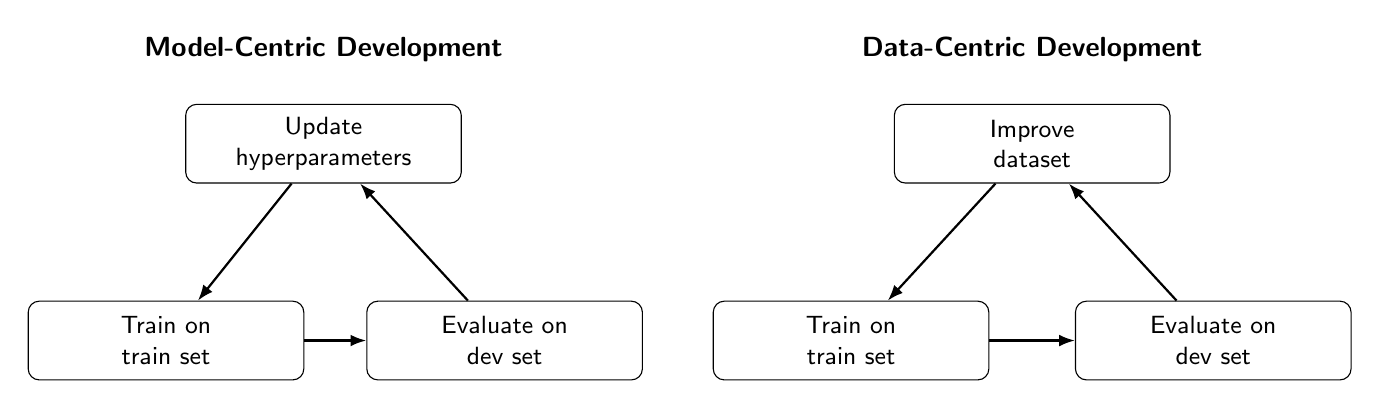
\begin{tikzpicture}[
    every node/.style={font=\small},
    box/.style={draw, rounded corners, align=center, minimum width=3.5cm, minimum height=1cm},
    arrow/.style={-{Latex[length=2mm]}, thick}
]

% --- Model-centric triangle ---
\node[font=\bfseries] at (-6.5, 5.2) {Model-Centric Development};
\node[box] (m_hyper) at (-6.5, 4) {Update \\ hyperparameters};
\node[box] (m_train) at (-8.5, 1.5) {Train on \\ train set};
\node[box] (m_eval) at (-4.2, 1.5) {Evaluate on \\ dev set};

\draw[arrow] (m_hyper) -- (m_train);
\draw[arrow] (m_train) -- (m_eval);
\draw[arrow] (m_eval) -- (m_hyper);

% --- Data-centric triangle ---
\node[font=\bfseries] at (2.5, 5.2) {Data-Centric Development};
\node[box] (d_data) at (2.5, 4) {Improve \\ dataset};
\node[box] (d_train) at (0.2, 1.5) {Train on \\ train set};
\node[box] (d_eval) at (4.8, 1.5) {Evaluate on \\ dev set};

\draw[arrow] (d_data) -- (d_train);
\draw[arrow] (d_train) -- (d_eval);
\draw[arrow] (d_eval) -- (d_data);

\end{tikzpicture}
\caption{Model-centric development updates the model while keeping the data fixed, whereas data-centric development improves the dataset while keeping the model fixed.}
\label{fig:model-vs-data-centric}
\end{figure}


Figure~\ref{fig:catboost-benchmark} illustrates a benchmark from the CatBoost website, comparing several gradient boosting frameworks across a range of classification tasks. While the original intention was to highlight CatBoost’s superior performance, a secondary takeaway is equally important: in most cases, tuning the hyperparameters led to only marginal improvements over default settings. This underscores a central motivation behind data-centric model development — when model tuning brings limited returns, improving the dataset itself becomes the more promising path forward.


\begin{figure}[H]
    \centering
    \includegraphics[width=0.95\textwidth]{data_figures/catboost_benchmark_barplots.png}
    \caption{
    Logloss values (lower is better) for a range of classification tasks as presented on the official \href{https://catboost.ai/}{CatBoost website} (accessed 5th April 2025). Each row corresponds to a dataset, and each column to a different gradient boosting framework (CatBoost, LightGBM, XGBoost, H2O). Within each cell, the blue bar represents the result using tuned hyperparameters, while the red bar corresponds to default settings. While the benchmark was designed to demonstrate CatBoost’s superior performance, a secondary observation is that in most cases, tuning had minimal impact—highlighting the surprising strength of default hyperparameters in practical scenarios.
    }
    \label{fig:catboost-benchmark}
\end{figure}





\section{Data Cleaning}

Data cleaning is a fundamental step in any machine learning pipeline. Poor data quality can lead to misleading patterns and reduce the effectiveness of even the most advanced models. This process typically involves handling missing values, identifying and removing outliers, correcting logically inconsistent entries, and ensuring uniform data formatting. \newline

\subsection{Dealing with Missing Values}
Missing values can arise from data collection issues, sensor failures, or human errors. The most common approaches to handle missing data include:

\begin{itemize}
    \item \textbf{Deletion:} Removing rows or columns with excessive missing values.
    \item \textbf{Imputation:} Filling missing values using methods like mean, median, or predictive models.
    \item \textbf{Using Algorithms That Handle Missing Data:} Some models, like decision trees, can work with missing values without explicit imputation.
\end{itemize}

\begin{examplebox}
Suppose a dataset contains patient records where 5\% of blood pressure readings are missing. A simple strategy is to impute missing values using the median blood pressure, as it is robust to outliers. However, if the missing values are not random (e.g., patients with higher blood pressure are more likely to have missing values), imputation may introduce bias.
\end{examplebox}

\subsection{Outlier Detection and Removal}
Outliers can distort model predictions, leading to inaccurate conclusions. Common techniques for detecting outliers include:

\begin{itemize}
    \item \textbf{Z-score Method:} Identifies points more than a specified number of standard deviations from the mean.
    \item \textbf{Interquartile Range (IQR):} Flags values outside 1.5 times the IQR as potential outliers.
    \item \textbf{Isolation Forests:} A machine learning approach that isolates anomalies using decision trees.
\end{itemize}

\noindent\begin{minipage}{\textwidth}
\begin{examplebox}
A real estate dataset contains house prices, with most values ranging between \$100,000 and \$500,000. However, a few properties are listed at \$50 million. These extreme values may be outliers resulting from data entry errors or genuinely expensive properties. Before removing them, one should analyze whether these values are meaningful in the given context.
\end{examplebox}
\end{minipage}

\subsection{Correcting Logically Inconsistent Data}
In some cases, data entries contain contradictions or impossible values. These must be corrected or removed to prevent erroneous model predictions.

\begin{examplebox}
A dataset on apartment listings contains an entry stating that an apartment is on the 7th floor of a building with only 5 floors. This inconsistency must be resolved, either by cross-referencing with other data or flagging the entry for removal.
\end{examplebox}

\subsection{Standardizing Data Formats}
Inconsistent formats can cause issues during model training. Standardization includes:

\begin{itemize}
    \item Converting \textbf{dates} into a uniform format (e.g., YYYY-MM-DD).
    \item Ensuring \textbf{categorical labels} are consistent (e.g., mapping "Male" and "M" to a single category).
    \item Unifying \textbf{measurement units} (e.g., converting all weights to kilograms).
\end{itemize}

\begin{examplebox}
A dataset tracking global temperatures records values in Celsius for some entries and Fahrenheit for others. Before modeling, all temperatures should be converted to a single unit to ensure consistency.
\end{examplebox}

Effective data cleaning enhances model reliability and ensures that patterns in the data accurately reflect real-world relationships rather than noise. \newline



\section{Handling Class Imbalances in Data}

Class imbalances can occur in both features and target variables. While target imbalances are well-known for causing model bias, imbalanced feature distributions can also impact learning. Below are concise guidelines on when these issues must be addressed and how to mitigate them.

\subsection{Imbalanced Feature Categories}

\textbf{When to Address It:}
\begin{itemize}
    \item If rare categories contain important information and the model fails to generalize.
    \item If one-hot encoding results in excessive sparsity due to highly imbalanced categories.
    \item If models relying on distance metrics (e.g., k-NN, clustering) suffer from poorly represented categories.
    \item If feature imbalance leads to implicit bias toward frequent categories.
\end{itemize}

\textbf{How to Address It:}
\begin{itemize}
    \item \textbf{Group Rare Categories:} Combine low-frequency categories into an "Other" category.
    \item \textbf{Target Encoding:} Encode categories based on mean target value (use cross-validation to avoid leakage).
    \item \textbf{Embedding Representation:} Use learned embeddings for categorical variables in deep learning models.
    \item \textbf{Reweighting Strategies:} Assign higher importance to rare categories in models that support weighting.
    \item \textbf{Synthetic Data Augmentation:} Generate synthetic samples to balance representation.
\end{itemize}

\begin{examplebox}
A retail company builds a recommendation system using customer location as a feature. Most customers are from urban areas, while only a few are from rural regions. Without adjustments, the model heavily favors urban preferences and fails to make meaningful recommendations for rural users. Grouping rural locations together or using embeddings can help mitigate this issue.
\end{examplebox}

\subsection{Imbalanced Target Classes}

\textbf{When to Address It:}
\begin{itemize}
    \item If the model favors the majority class and performs poorly on the minority class.
    \item If precision-recall trade-offs are critical (e.g., fraud detection, medical diagnosis).
    \item If the minority class is underrepresented to the point of ineffective learning.
\end{itemize}

\textbf{How to Address It:}
\begin{itemize}
    \item \textbf{Resampling:} Oversample the minority class (e.g., SMOTE) or undersample the majority class.
    \item \textbf{Class Weighting:} Assign higher loss weights to the minority class in models that support it.
    \item \textbf{Threshold Tuning:} Adjust decision thresholds to balance precision and recall.
    \item \textbf{Ensemble Methods:} Use balanced bagging or boosting approaches.
    \item \textbf{Anomaly Detection Approach:} If the minority class is extremely rare, treat it as an anomaly detection problem instead.
\end{itemize}

\begin{examplebox}
A bank develops a fraud detection system where fraudulent transactions make up only 0.1\% of all transactions. A model trained without addressing this imbalance predicts almost all transactions as non-fraudulent, achieving high accuracy but failing its purpose. Using SMOTE to oversample fraud cases and adjusting the classification threshold improves detection.
\end{examplebox}


\subsection{Conclusion}

Addressing class imbalances correctly improves model performance, ensures better generalization, and prevents bias toward dominant categories. Always validate chosen strategies through cross-validation and performance metrics tailored to the problem (e.g., F1-score, AUC-PR).



\section{Understanding Colliders, Confounders, and Mediators}

Many machine learning models rely on feature-target correlations without considering underlying causal relationships. However, blindly using correlated features can lead to spurious conclusions and harm generalization. This section explains three key concepts—colliders, confounders, and mediators—and when to drop certain features.

\subsection{Key Takeaways}
\begin{itemize}
    \item If a feature is a \textbf{collider}, it should typically be removed to prevent spurious correlations.
    \item If a feature is a \textbf{confounder}, adjusting for it (e.g., by adding related features) is recommended.
    \item If a feature is a \textbf{mediator}, retaining it depends on the modeling goal: include it for causal inference, but reassess for prediction tasks.
\end{itemize}


\subsection{Colliders}

A \textbf{collider} is a variable that is caused by two independent factors. When you condition on a collider (e.g., include it as a feature or filter data based on it), it can create a spurious correlation between these independent factors, even though they are not causally related.

\begin{examplebox}
Consider job hiring decisions. Both \texttt{Education Level} and \texttt{Social Connections} influence whether a person gets hired, but they do not directly influence each other. If we only analyze people who were hired (i.e., condition on hiring decisions), we might see a negative correlation between education and connections: among those hired, people with lower education tend to have stronger connections, while those with higher education often have weaker connections. This misleading correlation arises only because we conditioned on a collider (hiring). Since a candidate typically needs either strong qualifications or strong connections to be hired, those who lack one are more likely to rely on the other. As a result, individuals who lack formal education but were hired likely had strong social connections, while highly educated individuals may have been hired based on their qualifications alone. Those who lacked both would not have been hired and, therefore, do not appear in the analysis, artificially creating the observed relationship.
\end{examplebox}

\textbf{Practical Implication:}

If a feature is identified as a collider, removing it can improve generalization.

Be cautious when including variables that are consequences of multiple causes.

\subsection{Confounders}

A \textbf{confounder} is a variable that influences both a feature and the target, creating a misleading association between them. When confounders are present, the model may learn a spurious relationship, leading to incorrect conclusions and poor generalization.
\newline

A confounder introduces uncertainty about whether an observed correlation reflects a true causal link or is simply due to the confounder’s influence. This occurs because the confounder is driving both the feature and the target, making it seem as though the feature itself is responsible for changes in the target when, in reality, it is not.

\begin{examplebox}
A study finds a strong correlation between coffee consumption and heart disease. However, smoking is a confounder because it influences both coffee consumption and heart disease. Smokers are more likely to drink coffee, and they also have a higher risk of heart disease. If smoking is not accounted for, the model may falsely attribute heart disease risk to coffee consumption when, in fact, the observed correlation is primarily due to smoking.
\end{examplebox}

\textbf{Practical Implication:}

If a feature’s relationship with the target is primarily due to a confounder, adjustments should be made to prevent misleading conclusions.
\newline

Confounders should be identified and controlled for through feature selection, statistical adjustments (e.g., regression modeling, stratification), or causal inference techniques.
\newline

If a confounder is unmeasured and cannot be accounted for, be cautious in interpreting feature-target relationships, as they may not reflect real causal effects.

\subsection{Mediators}

A \textbf{mediator} is a variable that transmits the effect of one feature onto the target. Unlike confounders, mediators lie along the causal pathway.

\begin{examplebox}
Exercise reduces body weight, which in turn lowers the risk of heart disease. Here, body weight is a mediator between exercise and heart disease. If body weight is removed from the model, the relationship between exercise and heart disease may be underestimated.
\end{examplebox}

\textbf{Practical Implication:}
- Mediators are often **informative** and should be retained if modeling causal relationships.
- If only predicting outcomes, consider whether including a mediator enhances generalization or introduces redundancy.

\subsection{Conclusion}

Understanding these relationships ensures better feature selection, reduces overfitting, and improves the generalization of machine learning models.



\section{Dataset Size and Dimensional Regimes}

In machine learning, dataset size is often described in loose terms such as ``small'', ``medium'', or ``large''. However, these labels are inherently context-dependent and should be treated as rough heuristics rather than strict classifications.

\subsection{Heuristic Classification of Dataset Size}

The size of a dataset can be broadly estimated based on the number of instances (\(n\)) and the number of features (\(p\)). For many classical machine learning algorithms, the following rough classification is commonly used:

\begin{itemize}
    \item \textbf{Small:} \(n < 1{,}000\)
    \item \textbf{Medium:} \(1{,}000 \leq n \leq 100{,}000\)
    \item \textbf{Large:} \(n > 100{,}000\)
\end{itemize}

These boundaries are not universal and depend on the algorithm in question. For example, \(k\)-Nearest Neighbors scales poorly with large \(n\), while deep neural networks typically require large datasets to generalize well. Furthermore, the memory and computational load also depend on the overall size of the data matrix, \(n \times p\), which can affect feasibility in practice.

\subsection{Dimensional Regimes: The Relationship Between \(n\) and \(p\)}

Beyond absolute size, the ratio between the number of instances and the number of features is often more critical for determining learning difficulty and model suitability. Three regimes are typically distinguished:

\paragraph{\(n \gg p\) --- \textit{Data-rich regime}}
This is the ideal setting for most machine learning models, including deep learning architectures and classical methods such as logistic regression or support vector machines.
\begin{itemize}
    \item Common in image classification, sensor data, and many business applications.
    \item Overfitting is less of a concern, provided that models are appropriately regularized.
    \item Most algorithms perform well due to sufficient sample support.
\end{itemize}

\paragraph{\(p \gg n\) --- \textit{High-dimensional, low-sample regime}}
This regime is challenging and commonly encountered in domains such as genomics, transcriptomics, and medical diagnostics.
\begin{itemize}
    \item The curse of dimensionality severely limits the effectiveness of distance-based methods like \(k\)-NN.
    \item Feature selection, regularization, or dimensionality reduction is often required.
    \item Overfitting is a major risk due to the high model complexity relative to available data.
\end{itemize}

\paragraph{\(n \approx p\) --- \textit{Balanced but fragile regime}}
This setting presents statistical ambiguity:
\begin{itemize}
    \item Model complexity and data support are closely matched, increasing sensitivity to noise and overfitting.
    \item Generalization is possible if the data is clean and the model is regularized.
    \item Careful cross-validation and model selection become essential.
\end{itemize}

\subsection{Implications for the ML Pipeline}

The categorization of data size and its dimensional regime is a critical diagnostic step during the data understanding phase. However, its implications are most directly felt during model selection and evaluation. It helps determine whether certain models are feasible, which preprocessing steps (e.g., dimensionality reduction) are necessary, and how to balance bias and variance in the learning process.






\section{Data Augmentation}

\subsection{The Role of Data Augmentation in Performance Improvement}

There is a useful conceptual framework for understanding how data augmentation can enhance the performance of a learning algorithm. This perspective is particularly helpful when deciding whether to use data augmentation or collect additional real-world data. 
\newline

Take speech recognition as an example. There are various types of background noise in speech data, such as plane noise, car noise, train noise, and machine noise. These noise types are primarily mechanical in nature. On the other hand, environments like cafes, libraries, and food courts introduce a different category of background noise—primarily human voices and interactions. 
\newline

In the figure below, the vertical axis represents performance, such as accuracy, while the horizontal axis conceptually represents the space of possible inputs. Speech with plane, car, and train noise is relatively similar in nature, while library, cafe, and food court noise form another group. The performance of a model can vary significantly depending on these noise types. Typically, machine learning models perform better in some environments than others. 
\newline

\begin{figure}[H]
    \centering
    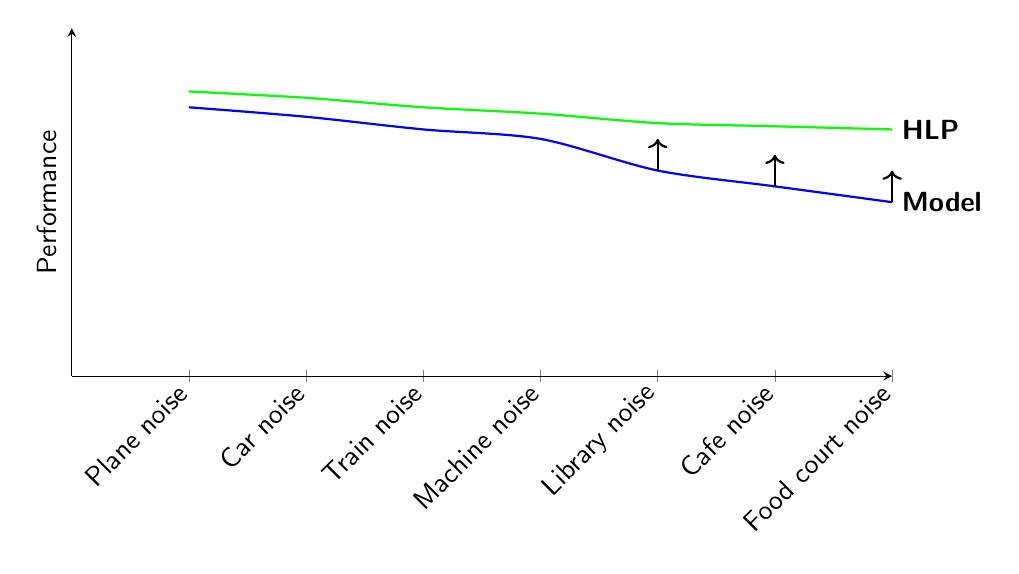
\begin{tikzpicture}
    \begin{axis}[
        ylabel={Performance},
        ymin=0, ymax=1.1,
        xmin=0, xmax=7,
        xtick={1,2,3,4,5,6,7},
        xticklabels={Plane noise, Car noise, Train noise, Machine noise, Library noise, Cafe noise, Food court noise},
        xticklabel style={rotate=45, anchor=east},  % Tilt x-axis labels
        ytick=\empty,
        enlargelimits=true,
        axis lines=left,
        clip=false,
        width=12cm,
        height=6cm
    ]
    
    % Human-level performance (HLP) curve
    \addplot[thick, green, smooth] coordinates {
        (1, 0.9) (2, 0.88) (3, 0.85) (4, 0.83) (5, 0.8) (6, 0.79) (7, 0.78)
    };
    \node[right, black] at (axis cs:7,0.78) {\textbf{HLP}};
    
    % Model performance curve
    \addplot[thick, blue, smooth] coordinates {
        (1, 0.85) (2, 0.82) (3, 0.78) (4, 0.75) (5, 0.65) (6, 0.6) (7, 0.55)
    };
    \node[right, black] at (axis cs:7,0.55) {\textbf{Model}};

    % Performance improvement arrows
    \addplot[->, thick, black] coordinates {(5, 0.65) (5, 0.75)};
    \addplot[->, thick, black] coordinates {(6, 0.6) (6, 0.7)};
    \addplot[->, thick, black] coordinates {(7, 0.55) (7, 0.65)};
    \end{axis}
\end{tikzpicture}

\caption{Model and human level performance (HLP) across different noise types.}
\label{fig:performance_rubber_band}
\end{figure}

As illustrated in the figure, human-level performance (HLP) is higher across all noise categories, whereas the model's performance (represented in blue) is lower, particularly in noisy human interaction settings like cafes and food courts. This gap represents an opportunity for improvement. 
\newline

If we apply data augmentation, or alternatively, collect additional data from environments where the model underperforms (e.g., cafes), we can effectively "pull up" the performance of the model in those regions. This concept can be visualized as stretching a rubber sheet upwards—improving one specific area tends to lift adjacent areas as well. 
\newline

For unstructured data problems, enhancing performance on one type of input is unlikely to significantly degrade performance on another. Instead, improvements in one region tend to propagate to nearby data points, whereas distant points may see a smaller improvement. When planning how to enhance a learning algorithm’s performance, this iterative approach of identifying weak regions, collecting additional data, and gradually pulling up performance is an efficient strategy. 
\newline

Once an area of significant performance gap has been closed, error analysis can help identify the next weak point, ensuring a systematic and data-driven improvement cycle. By focusing on data augmentation and targeted data collection, we can incrementally bring model performance closer to human-level performance in a structured and efficient manner.


\subsection{Designing Effective Data Augmentation Strategies}

Data augmentation is a powerful way to improve machine learning models, especially for unstructured data such as images, audio, and text. However, its effectiveness depends on how well it is designed. Choosing the right augmentation techniques requires careful consideration of parameters and a systematic approach to ensure they genuinely help the model learn better. \newline

Take speech recognition as an example. Suppose we have an audio clip saying, \textit{``AI is the new electricity.''} Adding background noise, such as cafe chatter, by summing the waveforms creates a synthetic example that mimics real-world noisy environments. Similarly, mixing speech with background music simulates conditions where someone is speaking with a radio playing. These types of augmentations allow us to efficiently expand our dataset without costly real-world data collection.

When implementing data augmentation, key decisions need to be made:
\begin{itemize}
    \item \textbf{Type of augmentation}: What variations should be introduced? For speech, should background noise, reverberation, or pitch shifts be applied? For images, should brightness, contrast, or geometric transformations be used?
    \item \textbf{Parameter tuning}: How strong should the augmentation be? For instance, in speech augmentation, determining the right volume level of background noise is crucial—too soft may not be useful, while too loud could make the audio incomprehensible.
    \item \textbf{Effectiveness validation}: How do we know if the augmented data is useful? One way is to ensure the augmented data meets three criteria:
        \begin{itemize}
            \item It should look or sound realistic.
            \item The mapping from input to output should remain clear (e.g., in speech, humans should still understand the words).
            \item The model should struggle on these examples initially, indicating room for improvement.
        \end{itemize}
\end{itemize}

An inefficient approach is to blindly apply data augmentation, train a model, and evaluate the performance afterward. Instead, a more structured approach is to sanity-check the augmented data before training. If the augmented data looks unnatural, is too distorted, or fails the criteria above, then retraining the model on such data may be a waste of time. \newline

For example, in image augmentation, flipping an image horizontally usually preserves meaning, but overly darkening it might make essential details unrecognizable (Figure~\ref{fig:good_and_bad_image_augmentation}). 

\begin{figure}[H]
    \centering
    \includegraphics[width=0.8\textwidth]{data_figures/good_and_bad_image_augmentation.png}
    \caption{Examples of effective and ineffective data augmentation for phone images. The top-right image is a horizontally flipped version of the original, while the middle-right image has been brightened—both preserving the visibility of scratches (the defect to be detected). In contrast, the bottom-right image has been darkened to the extent that the scratch is no longer visible to the human eye, making it unlikely for the algorithm to detect it. This illustrates an example of poor augmentation.}
    \label{fig:good_and_bad_image_augmentation}
\end{figure}

Similarly, artificially generating scratches on smartphone images using Photoshop can be an effective augmentation technique, as long as the added scratches remain realistic (Figure~\ref{fig:photoshop_augmentation}).

\begin{figure}[H]
    \centering
    \includegraphics[width=0.8\textwidth]{data_figures/photoshop_augmentation.png}
    \caption{Image augmentation using Photoshop: Realistic-looking scratches and other defects can be manually added to enhance training data.}
    \label{fig:photoshop_augmentation}
\end{figure}

Advanced augmentation techniques, such as Generative Adversarial Networks (GANs), can also synthesize new examples, but simpler methods often work just as well. Instead of spending excessive time on complex augmentation pipelines, focusing on simple, effective augmentations can yield substantial gains.

Beyond model iteration—where the model is refined through hyperparameter tuning and architecture improvements—a data iteration loop can be highly effective. This involves:
\begin{itemize}
    \item Performing error analysis to identify data gaps.
    \item Applying targeted data augmentation or collecting new data.
    \item Evaluating whether the model improves on the augmented data.
\end{itemize}

For many practical problems, taking this data-centric approach often leads to faster performance improvements than solely modifying the model. When error analysis reveals weaknesses in specific data subsets—such as speech with cafe noise—targeted data augmentation can efficiently address these gaps, improving model performance without requiring new architectures or complex model modifications.


\section{Can Adding Data Hurt?}

In many machine learning problems, the training, development, and test sets initially come from similar distributions. However, when using data augmentation, new data is often added to specific subsets of the training set—such as introducing more speech samples with cafe noise. This can shift the distribution of the training data significantly compared to the dev and test sets. Does this hurt the performance of a learning algorithm? Usually, the answer is no, with some important caveats. \newline

For unstructured data problems, adding accurately labeled data rarely degrades model accuracy under the following conditions:
\begin{itemize}
    \item The model has a sufficiently large capacity, such as a deep neural network with low bias.
    \item The mapping from input $x$ to output $y$ is clear, meaning that humans can confidently determine the correct label given only $x$.
\end{itemize}

As an example, consider a speech recognition model where, initially, 20\% of the dataset contains cafe noise. If augmentation increases this proportion to 50\%, the model’s input distribution has shifted. However, if the model is large enough, it can still generalize well across both cafe noise and non-cafe noise data. A smaller model, on the other hand, may struggle, allocating excessive capacity to modeling the cafe noise scenarios at the expense of general performance. \newline

A more unusual case where adding data could hurt is when the mapping from $x$ to $y$ is inherently ambiguous. This issue is rare in speech recognition but can arise in computer vision. Consider a system trained to recognize house numbers from Google Street View images. Most house numbers contain clear digits, but some characters are naturally ambiguous—such as a character that could be either the number “1” or the letter “I.” If many such ambiguous examples are added to the dataset, the model may struggle to learn the correct label assignment, as the distinction is unclear even to humans. This could introduce uncertainty into the model and lead to incorrect predictions, as it learns to treat these ambiguous cases differently than the intended real-world distribution. \newline

While such cases exist, they are rare. For most unstructured data problems, adding more training data—even if it alters the dataset distribution—tends to improve model performance, provided the model has sufficient capacity. Understanding these rare edge cases should give confidence in using data augmentation or expanding datasets to enhance algorithm performance.


\section{Collecting New Features}

Data augmentation is a powerful tool for unstructured data problems like images, audio, and text, but it is often ineffective for structured data, such as tables containing restaurant and customer information. Unlike in unstructured data, where new training examples can be synthesized, structured data problems typically involve a fixed set of entities, making it difficult to create new meaningful examples. Instead, improving structured data models often involves collecting new informative features. \newline

\begin{examplebox}
For instance, consider a restaurant recommendation system that predicts whether a user would like a specific restaurant. The system might use features describing both the user and the restaurant as inputs to a machine learning model. In one real-world example, error analysis revealed that vegetarians were frequently being recommended restaurants that only served meat-based dishes. This issue arose because the model lacked explicit features indicating whether a user was vegetarian or whether a restaurant had good vegetarian options.
\end{examplebox} 

Since the dataset has a fixed pool of users and restaurants, rather than attempting to generate synthetic data, a more effective solution is to collect new features that capture these critical distinctions. Features such as "percentage of vegetarian meals ordered by the user" or "restaurant has vegetarian options" help the model make better recommendations. These new features can be manually defined or automatically generated through techniques like natural language processing applied to restaurant menus. 



\section{Dropping Features}

In many cases, removing features from your dataset is not only justified—it’s essential. Features may need to be dropped because they introduce noise, redundancy, instability, or even dangerous leakage. A model trained on every available variable is not necessarily better; it may be overfit, less interpretable, or learning shortcuts that will fail in production.

\subsection{Avoid Hidden Leakage Through Metadata or Proxies}

One of the most critical reasons to drop a feature is label leakage. This occurs when a feature is strongly correlated with the label—but for the wrong reasons. These are often metadata or proxy variables that happen to align with the outcome during training, but won’t be present, meaningful, or stable at inference time.

Examples include:
\begin{itemize}
    \item File names or IDs that encode the label.
    \item Timestamps that coincide with label-generating events.
    \item Sensor IDs, annotator IDs, or devices used in data collection.
    \item Resolution, format, or data source differences that correlate with the target.
\end{itemize}

These “shortcuts” can dramatically inflate validation accuracy but lead to brittle models that collapse in real-world use. Always ask: \textbf{Would this feature still be available and behave similarly at inference time?}

\noindent\begin{minipage}{\textwidth}
\begin{examplebox}
In a hospital readmission prediction task, the model showed high accuracy—until it was discovered that discharge time was acting as a proxy for readmission. Overnight discharges were rare and often followed by urgent returns. The model had learned scheduling artifacts, not patient risk.
\end{examplebox}
\end{minipage}


\subsection{Drop Uninformative Features}

Some features simply don’t help the model—either because they carry no signal, or because their values barely vary across samples. Keeping such features increases noise, model complexity, and training time without any benefit.

Common candidates include:
\begin{itemize}
    \item Features with constant or near-constant values.
    \item Features with high missingness and no obvious imputation strategy.
    \item IDs, names, or random hashes with no predictive relevance.
\end{itemize}

\textbf{If a feature provides no useful variation, drop it. It only adds noise.}

\begin{examplebox}
In a customer churn dataset, the column “customer region” had 99.8\% of entries as “North America.” It added no useful signal and only served to distract the model. Dropping it improved training stability and interpretability.
\end{examplebox}




\chapter{Data-Centric Model Development 2: Feature Engineering}


Feature engineering refers to the \textbf{process of creating new features from existing ones} in order to improve the model’s ability to learn relevant patterns. Unlike simply adding more features from external sources, which expands the dataset’s information content, feature engineering involves transforming, combining, or encoding the available data to expose structure that models can exploit more effectively. It is a creative and often domain-informed process that can significantly impact model performance, especially when raw features are noisy, high-cardinality, or only indirectly informative.
\newline

\begin{notebox}
    Feature engineering primarily is relevant only for structured data (tables with explicit columns, like ``age'' and ``salary'').
\end{notebox}

In structured datasets, features are predefined variables, and the model's success often depends on how well these are crafted, encoded, and transformed. Feature engineering includes creating ratios, handling categorical variables, applying log or z-score transformations, or combining columns to reflect domain knowledge. These steps can dramatically influence performance, especially for traditional machine learning models.
\newline

For unstructured data — such as images, text, or audio — raw input is not organized into clear variables. In these cases, models like CNNs or transformers learn representations automatically, making manual feature engineering largely unnecessary. Instead, the focus shifts to preprocessing (e.g., tokenization, normalization) and choosing architectures that learn meaningful features from raw inputs.


Some examples for feature engineering:
\begin{itemize}
    \item \textbf{Loan Default Prediction:} Instead of using only raw income data, an effective feature might be the "Debt-to-Income Ratio," which normalizes a borrower’s debt by their income to better capture financial risk.
    \item \textbf{Fraud Detection:} Features like "number of transactions in the past 24 hours" or "percentage of transactions occurring in a foreign country" can help detect unusual spending behavior.
    \item \textbf{Customer Churn Prediction:} Metrics like "number of support tickets in the last month" or "days since last login" provide strong signals about potential customer churn.
\end{itemize}



\section{Transforming and Encoding Features}

Not all features speak the same language—models need help understanding the difference between categories, ordered categories, and numerical values. This chapter outlines how to transform or encode features depending on their measurement scale, with practical guidance tailored to downstream modeling.
\newline

The following table summarizes which type of transformation or encoding is typically appropriate for each feature scale:

\begin{table}[H]
\centering
\caption*{Which Features to Transform vs.\ Encode, Based on Measurement Scale}
\vspace{0.5em}
\renewcommand{\arraystretch}{1.4} % Adds vertical spacing between rows
\begin{tabular}{|l|p{3.8cm}|p{3cm}|p{5.2cm}|}
\hline
\textbf{Scale Type} & \textbf{Description} & \textbf{What to Do} & \textbf{Why} \\
\hline
Nominal & Categories with no intrinsic order (e.g., color, country). & Encode & Models cannot interpret raw category labels—must convert them into numbers. \\
\hline
Ordinal & Ordered categories (e.g., low < medium < high). & Encode (carefully) & Order can be meaningful, but spacing may not be. Use ordinal or target encoding when appropriate. \\
\hline
Interval & Numeric values without a true zero (e.g., temperature in °C). & Transform & Scale may be arbitrary; standardization or normalization often helps. \\
\hline
Ratio & Numeric values with a true zero (e.g., weight, height, income). & Transform & Ratios are meaningful; supports log, square root, and scaling transformations. \\
\hline
\end{tabular}
\renewcommand{\arraystretch}{1.0} % Reset row spacing
\end{table}


\subsection{Transforming Numerical Features}

Transformations help numerical features align better with model assumptions, stabilize gradients, and reduce sensitivity to outliers or scale differences. While tree-based models are scale-invariant, many others—such as logistic regression, SVMs, neural networks, and KNN—require properly scaled inputs to perform reliably.
\newline

Start by identifying which features are measured on an interval or ratio scale. Then decide whether to apply a transformation, based on the model type and data distribution.
\newline

\textbf{Common transformations:}
\begin{itemize}
    \item \textbf{Z-score standardization}: Subtract mean and divide by standard deviation. Use when features follow a roughly Gaussian distribution.
    \item \textbf{Min-max scaling}: Rescales features to a fixed range (e.g., 0 to 1). Useful when inputs have known bounds or when interpreting weights matters.
    \item \textbf{Robust scaling}: Uses median and IQR instead of mean and standard deviation. More stable when outliers are present.
    \item \textbf{Log or square root transforms}: Reduce skew for heavy-tailed distributions. Only apply to strictly positive data.
\end{itemize}

\begin{notebox}
Transformations must be applied \textbf{individually to each feature (column)}, not across rows. Scaling rows (i.e., per sample) destroys the feature structure and makes the data meaningless for modeling. 
\end{notebox}

\begin{notebox}
Transformations should be \textbf{fit on the training set only}, then applied to validation and test sets. Fitting on the full dataset introduces information leakage and gives overly optimistic results.
\end{notebox}

\begin{examplebox}
In a credit scoring model using logistic regression, the raw income feature ranged from hundreds to millions. Without scaling, the optimization algorithm failed to converge. Applying a log transform followed by standardization resolved the issue and significantly improved performance.
\end{examplebox}


\subsection{Encoding Categorical Features}

Most machine learning models require categorical features to be transformed into numerical representations before training. However, some models can handle categorical variables natively—understanding when and how to encode depends on both the feature type and the algorithm used. \newline

At the very beginning, always ask yourself whether the model you intend to use already handles categorical variables implicitly. If yes, you often don’t need to do anything. Tree-based models (e.g., decision trees, random forests, gradient boosting frameworks like LightGBM or XGBoost) can process categorical features directly if they are correctly specified. CatBoost goes a step further, using target statistics and permutations internally to encode categorical features without manual preprocessing. For these models, one-hot encoding is often unnecessary or even counterproductive. If the framework supports native categorical handling (as in LightGBM or CatBoost), it’s usually better to specify the categorical columns directly. \newline

Other models, however, do require explicit encoding of categorical features, such as:
\begin{itemize}
    \item Linear models (e.g., logistic regression)
    \item Distance-based models (e.g., KNN)
    \item SVMs
    \item Neural networks (if no embedding layer is used)
\end{itemize}

For these models, categorical features must be encoded into numerical form. The encoding strategy depends on whether the feature is nominal (no meaningful order) or ordinal (ordered categories), and on the number of unique levels. \newline

\textbf{Common encoding strategies:}
\begin{itemize}
    \item \textbf{One-hot encoding:} Creates a binary column for each category. Safe and widely used for nominal features, but can explode dimensionality with high-cardinality variables.
    \item \textbf{Ordinal encoding:} Maps categories to integers. Useful for ordinal features with meaningful order (e.g., low < medium < high), but misleading if applied to nominal features.
    \item \textbf{Target encoding:} Replaces each category with the mean target value (smoothed). Powerful but risky—must be applied with cross-validation or on training data only to avoid leakage.
    \item \textbf{Frequency or count encoding:} Replaces each category with its frequency or count in the dataset. Fast and often effective for high-cardinality features.
    \item \textbf{Hashing:} Maps categories into a fixed number of bins using a hash function. Useful when memory is constrained or categories are numerous and volatile.
    \item \textbf{Embeddings:} Represent categories as dense vectors learned during model training. Especially useful for high-cardinality features in neural networks, embeddings reduce dimensionality while allowing the model to learn similarity relationships between categories.
\end{itemize}

In all cases, ensure the encoding is applied consistently across train/validation/test splits, and avoid fitting encoders on the full dataset to prevent information leakage. \newline

\begin{examplebox}
A user behavior dataset contained a “country” column with over 200 levels. One-hot encoding created hundreds of sparse columns, overwhelming a logistic regression model. Switching to target encoding with proper cross-validation improved performance and reduced memory usage dramatically.
\end{examplebox}



\subsubsection{Target Encoding: Leveraging Category-Level Signal}

High-cardinality categorical variables can be challenging to use directly, especially when their categories lack inherent order or structure. Target encoding provides a powerful alternative: it replaces each category with the average value of the target variable observed for that category. This transforms a sparse, hard-to-learn categorical feature into a dense, informative numerical one.
\newline

Target encoding is especially useful when the categorical variable has many distinct values, such as region IDs, user IDs, or item IDs. Instead of requiring the model to learn one-hot representations or embeddings, target encoding allows the model to directly see how predictive each category is based on historical data.
\newline

However, target encoding must be applied with care. Since it uses information from the target variable, it can lead to data leakage if done naively. Always compute target encodings using only training data or within cross-validation folds.
\newline

In place of the mean, you can also use alternative aggregations to encode each category:
\begin{itemize}
  \item \textbf{Median target value} — more robust to outliers.
  \item \textbf{Smoothed mean} — blends the global mean and category mean to avoid overfitting in rare categories.
  \item \textbf{Target distribution probabilities} — encode the full class distribution per category (useful for classification).
  \item \textbf{Frequency or count encoding} — if you don’t want to use the target at all, but still need dense numeric features.
\end{itemize}

\begin{examplebox}
In a dataset of buildings affected by the Gorkha earthquake, each building has a \texttt{geo\_level\_3\_id} indicating its location. While the exact meaning of the IDs is not known, they carry strong predictive signal about the level of damage. If used directly as a categorical feature, the model would need to learn 12,567 separate rules—one for each unique region. Instead, we compute the average damage level (on a scale from 1 to 3) for each \texttt{geo\_level\_3\_id} and replace the original ID with this average. This transforms a high-cardinality categorical feature into a single dense numerical feature, drastically reducing dimensionality while preserving its predictive power.
\end{examplebox}


\section{Using Cluster Membership as a Feature}

Cluster membership can be added as a feature for supervised modeling. This is useful when the clusters capture higher-order structure that isn't obvious from the raw variables. Apply this when you suspect the model might benefit from latent groupings in the data, such as temporal states, cell populations, or condition clusters.

Always treat cluster labels as categorical; if your model doesn’t handle this natively, use one-hot encoding. Perform clustering only on the training data to avoid leaking structure into the test set.

\begin{examplebox}
You cluster omics samples into 5 groups based on expression profiles. These cluster assignments are then one-hot encoded and added as features in a regression model predicting drug response. The added structure improves model generalization.
\end{examplebox}



\section{Feature Splitting}

Complex or compound features—such as timestamps, strings, or encoded identifiers—often contain multiple sources of information bundled together. Feature splitting refers to the process of decomposing these into simpler, more interpretable components that can be modeled more effectively.

For example, a timestamp field can be split into \texttt{year}, \texttt{month}, \texttt{day}, \texttt{hour}, or even binary indicators like \texttt{is\_weekend}. A long text string might be split into \texttt{word\_count}, \texttt{avg\_word\_length}, or \texttt{contains\_keyword}. Similarly, location identifiers may encode hierarchical structure (e.g., region, district, block), which can be extracted into separate features.

This technique increases feature granularity and can expose hidden signals that would otherwise be lost or underutilized in raw compound formats.



\section{Polynomial Feature Generation}

While linear models are easy to interpret and efficient to train, they inherently assume linear relationships between features and the target variable. This assumption often fails in real-world data, where interactions and nonlinear effects are common.

Polynomial feature generation expands the feature space by adding higher-order combinations of numerical features, such as squared terms (\(x^2\)), interaction terms (\(x_1 \cdot x_2\)), or even cubic and beyond. These new features enable linear models to approximate nonlinear functions by capturing curvature and feature interactions implicitly.

Caution is advised: polynomial expansion can lead to rapid growth in dimensionality and increased risk of overfitting, especially when applied blindly to high-cardinality data. Regularization techniques or feature selection may be necessary to manage complexity.



\section{Binning}

Binning, also known as discretization, converts continuous numerical features into categorical bins. This is especially useful when the relationship between a feature and the target is non-monotonic or when the model struggles with continuous value ranges.

Common strategies include:
\begin{itemize}
    \item \textbf{Equal-width binning}: divides the feature range into intervals of equal size.
    \item \textbf{Quantile binning}: ensures each bin contains approximately the same number of observations.
    \item \textbf{Custom binning}: based on domain knowledge (e.g., age groups).
\end{itemize}

Binning can improve model stability, handle outliers more gracefully, and allow tree-based models to focus on split thresholds that align with real-world interpretations. However, it may also reduce resolution and lead to information loss if applied too aggressively.



\section{Feature Interaction Engineering}

Many real-world phenomena are governed not just by individual features but by their interactions. Feature interaction engineering explicitly creates new features that capture relationships between pairs or groups of existing features.

Examples include:
\begin{itemize}
    \item Multiplying numerical features: \texttt{area} = \texttt{height} $\times$ \texttt{width}
    \item Concatenating categorical features: \texttt{region\_district} = \texttt{region} + ``\_'' + \texttt{district}
    \item Creating logical combinations: \texttt{is\_young\_and\_employed} = \texttt{age < 30 \&\& employment == 1}
\end{itemize}

These engineered features can uncover patterns not visible to the model when considering variables in isolation. This technique is especially powerful in linear models, which cannot learn multiplicative or combinatorial effects by default. However, excessive interaction terms can lead to dimensional explosion and should be guided by domain knowledge or data-driven heuristics.


\section{Dimensionality Reduction}

High-dimensional datasets can lead to overfitting, increased computational cost, and degraded model performance. Dimensionality reduction aims to reduce the number of input features while preserving the most important information.

There are two main approaches:
\begin{itemize}
    \item \textbf{Feature selection}: retains a subset of the original features based on relevance (e.g., mutual information, variance threshold, model-based importance).
    \item \textbf{Feature extraction}: transforms the original features into a lower-dimensional space (e.g., Principal Component Analysis, t-SNE, Autoencoders).
\end{itemize}

This process is especially useful when dealing with sparse data, multicollinearity, or noisy features. While it can improve generalization and speed up training, it often comes at the cost of interpretability—particularly when using transformations like PCA or deep representations.



\section{Creating Indicator Features}

Indicator features are binary flags that highlight the presence of specific conditions, categories, or anomalies in the data. These features are especially useful when certain values or events carry disproportionate predictive power.

Common use cases include:
\begin{itemize}
    \item \textbf{Missingness indicators}: flag whether a value is missing, which can itself be informative.
    \item \textbf{Threshold flags}: e.g., \texttt{is\_high\_income} = \texttt{income > 100000}
    \item \textbf{Category presence}: e.g., \texttt{is\_police\_station} = 1 if \texttt{building\_use} == ``police''
\end{itemize}

These features are easy to interpret and can highlight edge cases or exceptional instances that the model might otherwise underweight. They are especially helpful in noisy, heterogeneous datasets or when building interpretable models.


\section{Conclusion}

Unlike unstructured data, where deep learning models learn features automatically, structured data often benefits from explicitly designed features, especially when dataset sizes are moderate. While large-scale deep learning models may eventually eliminate the need for manual feature engineering, for most real-world structured data applications, adding well-designed features remains a crucial technique for improving model accuracy and robustness.





\chapter{Dataset Versioning}

In any real-world machine learning project, datasets evolve over time: new features are added, preprocessing methods change, and additional sources are integrated. Keeping track of these versions in a clear and reproducible way is essential to ensure transparency and reliability throughout the modeling pipeline.



\section{Tree-based System}

This section introduces a lightweight, tree-based system for organizing and naming datasets along with metadata tracking. 


\subsection{Underscore-path naming convention}

Each dataset version name encodes its modification lineage using an underscore-separated format. Each code in the path represents a specific step or operation applied to the data. The path is read from left to right, with each new code indicating a modification built upon the previous one. All codes used in a version name must be defined in the modification glossary.
\newline

For example:

\begin{itemize}
    \item \texttt{trainR99} -- training split (99\% of raw data)
    \item \texttt{trainR99\_teG} -- added target encoding
    \item \texttt{trainR99\_teG\_ohe} -- added one-hot encoding
\end{itemize}

And separately for the dev set:

\begin{itemize}
    \item \texttt{devR1} -- dev split (1\% of raw data)
    \item \texttt{devR1\_teG} -- added target encoding
    \item \texttt{devR1\_teG\_ohe} -- added one-hot encoding
\end{itemize}




\subsection{Modification glossary}
This table defines the meaning of each code used in dataset version names:
\newline

\renewcommand{\arraystretch}{1.3}
\begin{tabular}{|l|p{9.5cm}|p{4.2cm}|}
\hline
\textbf{code} & \textbf{description} & \textbf{script} \\
\hline
trainR99 & 99\% of raw data used as train set (random split) & \texttt{split\_raw\_data.py} \\
devR1    & 1\% of raw data used as dev set (random split) & \texttt{split\_raw\_data.py} \\
teG       & Target encoding for geo features & \texttt{target\_encode\_geo.py} \\
ohe      & One-hot encoding for categoricals & \texttt{one\_hot\_encode.py} \\
\hline
\end{tabular}
\newline
\newline

Each code must be unique, and each modification should represent a single, well-defined change. Accordingly, each code in the version name should correspond to exactly one script that performs that specific step. Avoid combining multiple changes into a single modification (e.g.\ \texttt{tohe} \(\rightarrow\) \texttt{target\_and\_one\_hot\_encode.py}); instead, apply each change separately with one script per step. This ensures modularity, clarity, and scalability in dataset versioning.



\subsection{Version table}
This table logs each dataset version and its associated metadata:
\newline

\renewcommand{\arraystretch}{1.3}
\begin{tabular}{|l|p{2.5cm}|p{2.5cm}|p{5.5cm}|}
\hline
\textbf{version} & \textbf{date} & \textbf{person} & \textbf{comment} \\
\hline
v1 & 2025-03-29 & Thomas & Initial split (1\% dev) \\
v1\_te & 2025-03-29 & Thomas & Added target encoding \\
v1\_teG\_ohe & 2025-03-29 & Thomas &  \\
v1\_teG\_ohe\_ext & 2025-03-30 & Thomas & Added external features \\
\hline
\end{tabular}


\subsection{Example: Project Directory Structure}

The following example illustrates how this dataset versioning system is applied in a real project. The directory structure is organized as follows:

\begin{verbatim}
project/
|- data/
   |- raw/
   |  |- data_values.csv
   |  |- data_labels.csv
   |  |- test_values.csv
   |- modified/
      |- modification_glossary.csv
      |- version_table.csv
      |- datasets/
         |- trainR99.csv
         |- trainR99_ohe.csv
         |- devR1.csv
         |- devR1_ohe.csv
\end{verbatim}


\begin{itemize}
    \item The \texttt{raw} directory contains the original input files provided by the company. These are immutable.
    \item \texttt{data\_values.csv} and \texttt{data\_labels.csv} are merged and split to create \texttt{trainR99.csv} (99\% of the data) and \texttt{devR1.csv} (1\% of the data).
    \item The combined CSV files (e.g., \texttt{trainR99.csv}) contain both features and target labels, with the ID as the first column and the label as the last.
    \item \texttt{test\_values.csv} contains unlabeled data for model testing or submission.
    \item The \texttt{modified} directory holds all derived datasets and tracking metadata.
    \item \texttt{modification\_glossary.csv} defines all codes used in dataset version names.
    \item \texttt{version\_table.csv} logs when and why each version was created, by whom, and with what intent.
    \item The \texttt{datasets/} subfolder contains all versioned datasets as CSV files, named according to the underscore-based convention.
\end{itemize}

This setup enforces a clean separation between raw inputs and modified versions, while providing a transparent audit trail of how each dataset was generated.



\chapter{Data Tools}

\section{Overview: The Role of Tools in Data-Centric Work}

In real-world machine learning, data rarely arrives clean, small, and ready to model. The tools used to store, access, transform, and version data are crucial—sometimes more important than the model itself.

Unlike in academic settings where datasets are static and preprocessed, in applied ML projects, choosing the right data tools is a strategic decision. It affects development speed, reproducibility, and scalability. \newline

This chapter provides a practical overview of data tools, with a focus on \textbf{what exists}, \textbf{when it’s useful}, and \textbf{why you might choose one over another}. The emphasis is not on technical setup or configuration, but on informed selection during a machine learning workflow. \newline

We organize tools by their primary function:
\begin{itemize}
    \item \textbf{Storage and Access:} Where and how the data lives
    \item \textbf{Querying and Extraction:} How to get the data out
    \item \textbf{Transformation and Cleaning:} How to prepare it for modeling
    \item \textbf{Versioning and Tracking:} How to make workflows reproducible
    \item \textbf{Integration:} How to connect tools and expose data downstream
\end{itemize}



\section{Storage}

The first decision is where your data lives. This choice impacts accessibility, scalability, and the range of tools available for downstream tasks. You typically don’t get to choose the storage format in a project, but you need to understand its implications.

\subsection*{Flat Files}

\textbf{CSV, Parquet, JSON, Excel} \newline
Used when datasets are small, tabular, and fit into memory. Flat files are ideal for local development, prototyping, and sharing. \newline
\textbf{When to use:} Early stages, ad-hoc experiments, or exporting subsets of larger databases. \newline
\textbf{Why not always:} Poor support for concurrency, schema evolution, or large-scale data.

\subsection*{Relational Databases (SQL)}

\textbf{PostgreSQL, MySQL, SQLite, Microsoft SQL Server} \newline
Reliable, structured storage for transactional or tabular data. You define schemas and query with SQL. \newline
\textbf{When to use:} Most structured data projects—especially when data comes from internal systems or multiple sources that require joins. \newline
\textbf{Why not always:} Scaling can become complex; not well suited for unstructured data.

\subsection*{Non-Relational Databases (NoSQL)}

\textbf{MongoDB, Cassandra, DynamoDB, Redis} \newline
Useful for storing nested, semi-structured, or key-value data. Often used in production pipelines or when schema flexibility is required. \newline
\textbf{When to use:} Event logs, web/app data, hierarchical documents, or high-throughput systems. \newline
\textbf{Why not always:} Less consistent query language, harder to enforce data integrity, poorer support for joins.

\subsection*{Data Lakes and Warehouses}

\textbf{BigQuery, Snowflake, Redshift, Databricks, Delta Lake} \newline
Designed for large-scale analytics across massive datasets. Support SQL-style querying, versioned tables, and compute separation. \newline
\textbf{When to use:} Large datasets shared across teams, cloud-scale analytics, time-travel queries. \newline
\textbf{Why not always:} Overhead for small projects, sometimes high cost and learning curve.

\begin{notebox}
If you're training ML models on structured business data, you will likely interact with a SQL-based warehouse (e.g., BigQuery or Snowflake) and a flat file export pipeline. Know how to extract and structure the data yourself.
\end{notebox}



\section{Access}

Once data is stored, you need to extract the right subset for modeling. Whether it lives in a warehouse, database, or file—efficient access is a fundamental skill.

\subsection*{SQL}

\textbf{Standard SQL (PostgreSQL, MySQL, SQLite)} \newline
The foundation of querying structured data. Know it well. \newline
\textbf{When to use:} Any structured relational source. \newline
\textbf{Strengths:} Precise, optimized for joins and filters. \newline
\textbf{Weaknesses:} Cumbersome for complex transformations.

\subsection*{SQL Extensions and Warehouse Dialects}

\textbf{BigQuery SQL, Snowflake SQL, Athena SQL} \newline
Cloud-specific SQL dialects with added features: UDFs, window functions, nested fields. \newline
\textbf{When to use:} Inside data warehouses. Syntax quirks matter.

\subsection*{DataFrames in Python or R}

\textbf{Pandas, Polars, dplyr} \newline
Excellent for in-memory filtering and transformations after querying. \newline
\textbf{When to use:} After extracting data from SQL or files. \newline
\textbf{Why not always:} RAM-limited, not scalable.

\subsection*{ORMs and Query Builders}

\textbf{SQLAlchemy, Django ORM, dbplyr} \newline
Encapsulate SQL in Python/R. Good for structured pipelines. \newline
\textbf{When to use:} When building ingestion systems or production code. \newline
\textbf{Why not always:} Abstracts away too much for ad-hoc work.

\subsection*{APIs (REST and GraphQL)}

\textbf{REST + JSON, GraphQL} \newline
For third-party and internal services exposing data via HTTP. \newline
\textbf{When to use:} If SQL access is restricted or you're working with SaaS platforms. \newline
\textbf{Why not always:} Not built for analytics. Fragile, rate-limited, often undocumented.

\begin{examplebox}
If your company uses Snowflake and dbt, you’ll write warehouse SQL to define reusable data models, and then extract them via Python with \texttt{snowflake.connector}.
\end{examplebox}




\section{Data Processing and Transformation Frameworks}

Once data is extracted, it often needs to be cleaned, merged, reshaped, or enriched. For anything beyond what fits in memory or involves many moving parts, you need a processing framework.

\subsection*{Pandas and Data.table}

\textbf{Pandas (Python) / Data.table (R)} \newline
Still the most common tools for in-memory data wrangling. Good for prototyping and medium-scale transformations. \newline
\textbf{When to use:} Local work on datasets that fit in memory. \newline
\textbf{Strengths:} Flexible, expressive, well-supported. \newline
\textbf{Limits:} RAM-bound, no built-in parallelism.

\subsection*{Polars and Dask}

\textbf{Polars:} A fast DataFrame library with Rust under the hood. \newline
\textbf{Dask:} Parallelizes NumPy/Pandas workflows across cores or clusters. \newline
\textbf{When to use:} If you're hitting memory limits or performance walls with Pandas. \newline
\textbf{Tip:} Use Polars for raw speed, Dask when working with larger-than-memory data.

\subsection*{Apache Spark (PySpark)}

\textbf{Spark} is the industry standard for distributed data processing. It scales across clusters and can handle terabytes. \newline
\textbf{When to use:} Transformations on huge datasets, building ETL pipelines, or working in a cloud data lake. \newline
\textbf{Strengths:} Scalable, fault-tolerant, integrates well with HDFS and cloud storage. \newline
\textbf{Drawbacks:} Verbose, hard to debug, overkill for small tasks.

\subsection*{dbt (Data Build Tool)}

\textbf{dbt} lets you define data transformations as modular SQL files. It brings software engineering practices (testing, versioning) to analytics pipelines. \newline
\textbf{When to use:} When your company uses a cloud data warehouse and your transformations are in SQL. \newline
\textbf{Why it matters:} It standardizes data modeling across teams.

\subsection*{Airflow and Workflow Orchestration}

\textbf{Apache Airflow, Prefect, Dagster} \newline
Orchestrate complex data workflows with clear dependencies and schedules. \newline
\textbf{When to use:} When you have many interdependent data tasks running daily or hourly. \newline
\textbf{Important:} These are not for processing data—they schedule and manage the things that do.

\begin{examplebox}
A typical data workflow might pull raw logs from S3, transform them in Spark, store the result in Snowflake, and use dbt to clean up the schema. Airflow schedules the whole thing hourly.
\end{examplebox}



\section{Versioning, Tracking, and Lineage}

In real-world machine learning projects, data is not static. It evolves—through cleaning, filtering, annotation, or as new samples arrive. Without tracking these changes, results become irreproducible and collaboration breaks down. Versioning and lineage tools help manage this complexity.

\subsection*{Why Versioning Matters}

\begin{itemize}
    \item Re-running a pipeline on a slightly modified dataset can lead to different results.
    \item Teams need to know which data version was used for a model.
    \item Debugging a model requires knowing the exact state of the data it saw during training.
\end{itemize}

\subsection*{Popular Tools}

\textbf{DVC (Data Version Control):} Git-like interface for tracking datasets and model artifacts.\newline
\textbf{LakeFS / Pachyderm:} Git-style versioning on top of object storage systems.\newline
\textbf{Delta Lake / Apache Hudi / Apache Iceberg:} Add versioning, rollback, and lineage to data lakes (often used with Spark).\newline
\textbf{MLflow Tracking:} While mainly used for experiment tracking, it can log datasets and parameters alongside models.

\subsection*{Best Practices}

\begin{itemize}
    \item Treat datasets as code: use commits, tags, and branches.
    \item Log metadata and processing steps alongside raw data.
    \item Always tie a model to a specific version of the dataset.
\end{itemize}

\begin{examplebox}
A company detected a model accuracy drop after retraining. Using DVC, they quickly traced the issue to a mislabeled sample introduced in a new dataset version—saving hours of debugging.
\end{examplebox}


\section{Interfacing and Integration}

A strong data stack doesn’t end at pipelines and storage—it needs to interface with users, applications, and stakeholders. Interfacing tools ensure that data flows smoothly between systems and people.

\subsection*{Cloud Data Platforms}

\textbf{Examples:} Snowflake, BigQuery, Redshift \newline

These platforms allow teams to run analytical queries on massive datasets with minimal infrastructure effort. They're commonly used in production environments for:

\begin{itemize}
    \item Fast querying across large tables.
    \item Feeding dashboards and reporting systems.
    \item Integrating with machine learning pipelines via connectors or APIs.
\end{itemize}

\subsection*{BI and Dashboards}

\textbf{Examples:} Tableau, Power BI, Superset \newline

Business Intelligence (BI) tools empower non-technical users to explore data and generate insights visually. They are most useful when:

\begin{itemize}
    \item Stakeholders need live reporting dashboards.
    \item Teams want to track metrics and KPIs without writing code.
    \item Data scientists need a fast way to explore structured data.
\end{itemize}

\begin{notebox}
Even if you're not directly building dashboards, understanding the BI stack helps align your work with how stakeholders consume insights.
\end{notebox}





\part{Modeling}



\chapter{Modeling Ordinal Target Variables}

In supervised learning, the nature of the target variable strongly influences
how a problem should be approached. There are four basic scale types:
\newline

\begin{minipage}{\textwidth}
\centering
\renewcommand{\arraystretch}{1.3} % Adjust row spacing
\begin{tabular}{m{2.5cm} m{1.5cm} m{4cm} m{7cm}}
\toprule
\textbf{Scale Type} & \textbf{Order} & \textbf{Distance} & \textbf{Examples} \\
\midrule
Nominal   & No  & No  & color, country, animal type \\
Ordinal   & Yes & No  & satisfaction rating (low, medium, high) \\
Interval  & Yes & Yes (no true zero)  & temperature in °C, calendar years \\
Ratio     & Yes & Yes (with true zero) & height, weight, income \\
\bottomrule
\end{tabular}
\end{minipage}
\vspace{5pt}


\vspace{10pt}

For most applications, the modeling strategy is straightforward:
\begin{itemize}
    \item \textbf{Nominal} → Classification
    \item \textbf{Interval/Ratio} → Regression
\end{itemize}

However, \textbf{ordinal target variables fall into a twilight zone} between 
classification and regression. They have a natural order, but the distances 
between categories are unknown or non-linear. This chapter presents a 
concise overview of common modeling strategies for ordinal targets, which are:

\begin{minipage}{\textwidth}
\begin{center}
\renewcommand{\arraystretch}{1.5} % <-- Increases vertical spacing between rows
\begin{tabular}{lp{9cm}}
\toprule
\textbf{Approach} & \textbf{When to Use} \\
\midrule
Treat as Classification & When the ordinal nature of the target is not critical \\
Use an Ordinal Classification Model & When you want an interpretable model that respect class ordering without complex tuning \\
Map to Integers and Regress & When the target can be meaningfully treated as a continuous scale (e.g., severity levels), and simple regression yields competitive results. Useful when exact ranking matters more than discrete class boundaries. \\
Regression with Ordinal-Aware Loss & When you're training flexible models (like trees or neural nets) and want to enforce that predicting “2” instead of “3” is better than predicting “5”. Ideal when minimizing the distance between predicted and true class is more important than raw accuracy. \\
Classification with Ordinal-Aware Loss & When you want discrete class outputs but still want the model to respect the ordinal structure during training. Useful when ordinal penalties matter but classification is preferred over regression. \\
Deep Learning with Ordinal Encoding & When using deep learning and you want the model to learn thresholds between classes explicitly, preserving ordinal structure without relying on regression tricks. Especially useful for problems with many ordered classes or noisy boundaries. \\
\bottomrule
\end{tabular}
\end{center}
\end{minipage}

\vspace{10pt}

\section{Strategy 1: Treat as Classification}

The simplest approach is to use a standard classification algorithm, ignoring
the order between classes.

\begin{itemize}
    \item Predicts discrete categories
    \item Does not use the ordinal information
    \item Allows to use powerful algorithms like XGBoost and Neural Networks.
\end{itemize}

\begin{examplebox}
A 3-class satisfaction label (`low`, `medium`, `high`) is treated as a
standard classification problem using logistic regression. The model
predicts class probabilities independently, which may result in
inconsistent or illogical class rankings.
\end{examplebox}

\vspace{5pt}

\section{Strategy 2: Use an Ordinal Classification Model}

Ordinal models explicitly respect the class order. The most common is
the \textit{proportional odds model} (ordinal logistic regression).

\begin{itemize}
    \item Predicts cumulative class probabilities
    \item Assumes a shared linear function with ordered thresholds
    \item Available in \texttt{MASS::polr} (R), 
          \texttt{statsmodels} (Python), and others
\end{itemize}

\begin{examplebox}
Using ordinal logistic regression to model education level (`primary`, 
`secondary`, `tertiary`) ensures that predictions maintain a logical 
ordering. The model estimates cumulative thresholds, e.g., 
$P(\text{level} \leq \text{secondary})$.
\end{examplebox}

\vspace{5pt}

\section{Strategy 3: Map to Integers and Regress}

Map classes to integers (e.g., `low` = 1, `medium` = 2, `high` = 3) and
train a regression model. Predictions are rounded to the nearest class.

\begin{itemize}
    \item Simple and often effective
    \item Assumes equal distance between classes
    \item Allows to use powerful algorithms like XGBoost and Neural Networks.
\end{itemize}

\begin{examplebox}
The ordinal target `bad`, `average`, `good`, `excellent` is mapped to 
$[1,2,3,4]$. A linear regression model predicts scores like 2.7, which are 
then rounded to predict `good`. Note that the spacing is assumed equal.
\end{examplebox}

\vspace{5pt}

\section{Strategy 4: Regression with Ordinal-Aware Loss}

You can use a regression model with a custom loss function that penalizes
ordering mistakes more heavily (e.g., predicting `1` when the true label is `4`).

\begin{itemize}
    \item Captures severity of misclassification
    \item More nuanced than plain MSE
    \item Can use techniques like Earth Mover's Distance
    \item Allows to use powerful algorithms like XGBoost and Neural Networks.
\end{itemize}

\begin{examplebox}
A model trained on movie ratings (1 to 5 stars) uses a custom loss that 
penalizes large prediction errors more than small ones. Predicting `1` 
instead of `5` is worse than predicting `4` instead of `5`.
\end{examplebox}

\vspace{5pt}


\section{Strategy 5: Classification with Ordinal-Aware Loss}

Instead of treating the problem as pure regression, you can stick with a classification model while modifying the loss function to respect the ordinal structure. This encourages the model to treat misclassifications proportionally to their severity.

\begin{itemize}
    \item Preserves discrete class outputs
    \item Penalizes distant class errors more than close ones
    \item Can be implemented via custom loss functions (e.g., MAE-style gradient)
    \item Compatible with models like XGBoost and Neural Networks
\end{itemize}

\begin{examplebox}
In an earthquake damage classification task (classes 1–3), an XGBoost model is trained using a custom loss that penalizes a prediction of `3` for a true class of `1` more than a prediction of `2`. This reflects the ordered nature of damage severity without switching to regression.
\end{examplebox}

\vspace{5pt}



\section{Strategy 6: Deep Learning with Ordinal Encoding}

Deep learning models can be adapted for ordinal targets by designing the output layer to reflect the \textbf{ordered structure} of the labels. Instead of predicting class probabilities with a softmax (which treats all classes as unrelated), these models use techniques like:

\begin{itemize}
    \item \textbf{Ordinal binary encoding} — the model predicts whether the target exceeds each threshold (e.g., ``Is it greater than class 1? Class 2?'' etc.).
    \item \textbf{CORAL} (Cumulative Ordinal Regression with Logistic Loss) — a principled approach that uses a shared representation with cumulative logistic functions at the output.
\end{itemize}

These methods impose ordinal structure \emph{directly into the network’s output}, ensuring that predictions respect the class order. This is especially valuable in deep learning, where custom output heads, shared representations, and complex data (images, text, sequences) make such modeling both feasible and effective.

\begin{examplebox}
Instead of predicting a softmax over 5 pain severity levels, a neural network outputs four binary decisions: “Is pain \textgreater{} 0?”, “\textgreater{} 1?”, “\textgreater{} 2?”, “\textgreater{} 3?”. This reflects the natural ordering and improves consistency across predictions.
\end{examplebox}


\vspace{10pt}



\chapter{Model, Objective, Optimization, and Evaluation}

Most data analysis methods comprise the following four steps:
\begin{itemize}
    \item \textbf{Select the model class} (e.g. linear regression)
    \item \textbf{Select the objective function} (e.g. mean squared error)
    \item \textbf{Apply the optimizer (optimization algorithm)} (e.g. gradient descent)
    \item \textbf{Validate the results using an evaluation metric} (e.g. $R^2$ score)
\end{itemize}


\section{Selecting a Model Class}

In the modeling stage of a machine learning project, choosing the right model class is a fundamental decision that affects predictive performance, interpretability, and computational efficiency. The model class defines the structure of the relationship between input data and predictions. Some models, such as linear regression, make strong assumptions about the underlying data, while others, like neural networks, provide more flexibility at the cost of complexity.
\newline

Key factors in selecting a model class include:
\begin{itemize}
    \item \textbf{Fit to Data:} How well the model captures underlying patterns.
    \item \textbf{Complexity vs. Interpretability:} Simpler models are easier to understand, but may fail to capture intricate patterns.
    \item \textbf{Computational Efficiency:} Some models require significant training time and resources.
    \item \textbf{Generalization Ability:} Overly complex models may overfit the training data.
    \item \textbf{Task-Specific Requirements:} The choice of model depends on whether the task is classification, regression, clustering, or reinforcement learning.
\end{itemize}

Model classes can be broadly grouped into four types, based on how they learn from data.

\begin{itemize}
    \item \textbf{Supervised Learning:} Learn from labeled input-output pairs. Use when labeled data is available and prediction is the goal.
    \item \textbf{Unsupervised Learning:} Find structure in unlabeled data. Use for clustering, dimensionality reduction, or anomaly detection.
    \item \textbf{Self-Supervised Learning:} Create pseudo-labels from raw data. Use when labeled data is scarce but large amounts of raw data exist.
    \item \textbf{Reinforcement Learning:} Learn via reward signals through interaction. Use for decision-making tasks with sequential feedback (e.g., games, robotics).
\end{itemize}


\subsection{Supervised Learning}

Supervised learning models are trained on labeled data, mapping inputs to known outputs.

\begin{table}[H]
    \centering
    \small
    \caption{Supervised learning models that treat features independently (no interaction modeling). Data type support (structured (S) or unstructured (U)) and training speed are indicated.}
    \resizebox{\textwidth}{!}{%
    \begin{tabular}{|p{2.2cm}|c|c|p{3.5cm}|p{3cm}|p{3cm}|p{1.8cm}|}
        \hline
        \textbf{Model Type} & \textbf{S} & \textbf{U} & \textbf{When to Use} & \textbf{Advantages} & \textbf{Disadvantages} & \textbf{Training Speed} \\
        \hline
        Linear Regression & \cmark & \xmark & When interpretability is very important and there is a linear relationship & Fast, interpretable, low variance & Assumes linearity, no interaction modeling unless manually added, can only be used for regression & \textbf{Very Fast} \\
        \hline
        Linear Discriminant Analysis (LDA) & \cmark & \xmark & When you need a fast, interpretable classifier that works well on small datasets with linearly separable classes & Captures some interactions via shared covariance, probabilistic output & Assumes normality and equal covariance across classes, limited to linear boundaries & \textbf{Fast} \\
        \hline
        Quadratic Discriminant Analysis (QDA) & \cmark & \xmark & When you need a more flexible classifier than LDA for small datasets with moderately non-linear, class-specific distributions & Models class-specific covariance, flexible decision boundaries & Requires more data, sensitive to overfitting, assumes Gaussian features & \textbf{Moderate} \\
        \hline
        Logistic Regression & \cmark & \xmark & Binary classification with simple features & Probabilistic output, interpretable coefficients & Linear decision boundaries only, no implicit interactions & \textbf{Fast} \\
        \hline
        K-Nearest Neighbors (KNN) & \cmark & \xmark & Small to medium datasets with local structure & No training time, easy to understand & Poor in high dimensions, sensitive to feature scale & \textbf{Slow (at inference)} \\
        \hline
        Naïve Bayes & \cmark & \xmark & Use Naive Bayes when you need a fast, simple, and interpretable model for high-dimensional, sparse, and small datasets with mostly independent features. Prime use cases are text classification, spam detection, and sentiment analysis. Can only be used for classification. & Extremely fast, works well on sparse data & Strong independence assumption, poor for correlated features, can only be used for classification & \textbf{Very Fast} \\
        \hline
    \end{tabular}
    }
\end{table}


\begin{table}[H]
    \centering
    \small
    \caption{Supervised learning models that model interactions between features. Data type support (structured (S) or unstructured (U)) and training speed are indicated.}
    \resizebox{\textwidth}{!}{%
    \begin{tabular}{|p{2.2cm}|c|c|p{3.5cm}|p{3cm}|p{3cm}|p{1.8cm}|}
        \hline
        \textbf{Model Type} & \textbf{S} & \textbf{U} & \textbf{When to Use} & \textbf{Advantages} & \textbf{Disadvantages} & \textbf{Training Speed} \\
        \hline
        Decision Tree & \cmark & \xmark & Simple structured data with non-linear rules & Interpretable, handles non-linearities & Unstable, prone to overfitting & \textbf{Fast} \\
        \hline
        Random Forest & \cmark & \xmark & Structured data with moderate complexity & Reduces overfitting, handles interactions well & Less interpretable, slower than single tree & \textbf{Moderate} \\
        \hline
        SVM & \cmark & \xmark & Small, high-dimensional datasets & Captures complex decision boundaries with kernels & Sensitive to scaling, hard to tune & \textbf{Slow} \\
        \hline
        XGBoost & \cmark & \xmark & Structured data with high accuracy demand & Top performance, regularization built-in & Slower to train, harder to tune & \textbf{Moderate} \\
        \hline
        CatBoost & \cmark & \xmark & Categorical-heavy structured data & Handles categoricals natively, minimal tuning & Slower training, less interpretable & \textbf{Moderate} \\
        \hline
        LightGBM & \cmark & \xmark & Large structured datasets where speed matters & Fastest boosting, good accuracy & Sensitive to tuning, less robust for small data & \textbf{Fast} \\
        \hline
        AdaBoost & \cmark & \xmark & Simple data with low noise & Easy to implement, interpretable base learners & Sensitive to noise, less powerful than XGBoost & \textbf{Fast} \\
        \hline
        NGBoost & \cmark & \xmark & When you need accurate predictions with well-calibrated uncertainty in complex, non-linear problems & Predictive distributions, interpretable outputs & Slower training, less known & \textbf{Slow} \\
        \hline
        Neural Networks & \cmark & \cmark & Unstructured or high-dimensional data & Models complex patterns, automatic feature learning & Black box, high compute cost, need for large datasets & \textbf{Slow} \\
        \hline
        Bayesian Neural Network & \cmark & \cmark & Like neural networks but when uncertainty estimation is critical & Quantifies uncertainty, regularization built-in & Complex to implement and scale & \textbf{Very Slow} \\
    \end{tabular}
    }
\end{table}


\subsection{Self-Supervised Learning}

Self-supervised learning extracts patterns from unlabeled data by generating 
pseudo-labels internally.

\begin{table}[H]
    \centering
    \small
    \renewcommand{\arraystretch}{1.3} % Better row spacing
    \begin{tabular}{|l|p{8cm}|}
        \hline
        \textbf{Model Type} & \textbf{When to Use} \\
        \hline
        Contrastive Learning & When learning feature representations from unlabeled data by comparing similar and dissimilar pairs. Best for image and speech representation learning. \\
        \hline
        Autoencoders & When performing unsupervised anomaly detection, dimensionality reduction, or data denoising. Often used in medical imaging and fraud detection. \\
        \hline
        Variational Autoencoders (VAE) & When generating new data samples similar to the training set (e.g., image synthesis) while also learning a meaningful latent representation. \\
        \hline
        Transformers (BERT, GPT) & When working with natural language processing (NLP) tasks such as text generation, translation, or sentiment analysis. Best for large-scale language models. \\
        \hline
        Denoising Autoencoders & When improving feature extraction from noisy input data. Used in speech recognition and image restoration tasks. \\
        \hline
        SimCLR & When using contrastive learning for self-supervised image representation learning. Works well when labeled images are scarce. \\
        \hline
        MoCo (Momentum Contrast) & When applying self-supervised contrastive learning for image classification with a memory-efficient approach. Useful for vision tasks with large-scale unlabeled datasets. \\
        \hline
        BYOL (Bootstrap Your Own Latent) & When learning high-quality feature representations without negative samples. Suitable for vision tasks with limited labels. \\
        \hline
        SwAV (Swapping Assignments between Views) & When performing self-supervised clustering and learning feature representations without explicit contrastive pairs. Best for image pretraining. \\
        \hline
    \end{tabular}
    \caption{Self-supervised learning models and when to use them.}
\end{table}


\subsection{Unsupervised Learning}

Unsupervised models identify patterns in data without labeled outputs, 
typically used for clustering or dimensionality reduction.

\begin{table}[H]
    \centering
    \small
    \renewcommand{\arraystretch}{1.3} % Better row spacing
    \begin{tabular}{|l|p{8cm}|}
        \hline
        \textbf{Model Type} & \textbf{When to Use} \\
        \hline
        K-Means Clustering & When grouping data into a predefined number of clusters. Best for well-separated, spherical clusters in low-dimensional data. \\
        \hline
        Hierarchical Clustering & When a hierarchy of clusters is needed and the number of clusters is not known in advance. Works well for dendrogram-based analysis. \\
        \hline
        Gaussian Mixture Models (GMM) & When modeling soft clustering, where each point belongs to multiple clusters with probabilities. Suitable for data with overlapping clusters. \\
        \hline
        DBSCAN (Density-Based Spatial Clustering) & When detecting clusters of varying shapes and densities, particularly with noise. Works well for geospatial and anomaly detection tasks. \\
        \hline
        Principal Component Analysis (PCA) & When reducing dimensionality while preserving variance. Best for visualization, noise reduction, and speeding up machine learning models. \\
        \hline
        t-SNE / UMAP & When performing non-linear dimensionality reduction for visualization. Best for exploring high-dimensional data, such as word embeddings or genomics. \\
        \hline
        Self-Organizing Maps (SOM) & When visualizing and clustering high-dimensional data in a low-dimensional space. Useful for pattern recognition and anomaly detection. \\
        \hline
        Isolation Forest & When detecting anomalies or outliers in high-dimensional datasets. Works well in fraud detection and cybersecurity. \\
        \hline
    \end{tabular}
    \caption{Unsupervised learning models and when to use them.}
\end{table}


\subsection{Reinforcement Learning}

Reinforcement learning models learn through interaction with an environment 
by maximizing rewards.

\begin{table}[H]
    \centering
    \small
    \renewcommand{\arraystretch}{1.3} % Better row spacing
    \begin{tabular}{|l|p{8cm}|}
        \hline
        \textbf{Model Type} & \textbf{When to Use} \\
        \hline
        Q-Learning & When solving simple reinforcement learning tasks with discrete state-action spaces. Best for low-dimensional problems where a Q-table can be maintained. \\
        \hline
        Deep Q-Networks (DQN) & When applying reinforcement learning to complex, high-dimensional environments (e.g., games, robotics). Uses neural networks to approximate Q-values. \\
        \hline
        Policy Gradient Methods (PPO, A3C) & When learning in continuous action spaces (e.g., robotics control). Best when explicit policy optimization is needed rather than relying on Q-values. \\
        \hline
        Actor-Critic Methods & When combining value-based and policy-based approaches for more stable learning. Works well in tasks requiring both exploration and exploitation. \\
        \hline
        AlphaZero-style Learning & When training an agent purely through self-play and Monte Carlo Tree Search (MCTS). Best for strategic games like chess and Go. \\
        \hline
        Multi-Agent Reinforcement Learning (MARL) & When solving problems where multiple agents interact in a shared environment, such as traffic simulations or economic modeling. \\
        \hline
        Model-Based Reinforcement Learning & When computational efficiency is important, as it attempts to learn a model of the environment. Useful in applications like robotics and planning. \\
        \hline
    \end{tabular}
    \caption{Reinforcement learning models and when to use them.}
\end{table}



\section{Selecting an Objective Function}

Choosing a model class defines the general structure of a model, 
typically in terms of a set of parameters. However, to determine 
the best or at least a good model for a given dataset, a 
\textbf{fitting criterion} is needed. This criterion is usually 
formulated as an \textbf{objective function}:

\ensuremath{f : M \to \mathbb{R}}

where \( M \) is the set of considered models. The objective function 
quantifies how well a model fits the data and guides the optimization 
process.

Before selecting an objective function, it is essential to identify 
the nature of your prediction task. Most machine learning problems 
can be broadly categorized as \textbf{regression}, 
\textbf{classification}, or \textbf{ordinal classification}—the latter 
sitting between the first two. Each of these categories requires 
different types of objective functions.

\begin{notebox}
The \textit{objective function} is minimized or maximized during training 
to guide the optimizer (e.g. MSE), while the \textit{evaluation metric} 
(e.g. $R^2$ or accuracy) is used after training to assess model performance 
and rank different sets of hyperparameters. A confusion between the two 
often arises because, for example in regression tasks, the same function (e.g. MSE) is 
commonly used both as the objective and the evaluation metric.
\end{notebox}


\subsection{Regression Objectives}

\begin{table}[H]
    \centering
    \small
    \renewcommand{\arraystretch}{1.3}
    \begin{tabular}{|l|p{9cm}|}
        \hline
        \textbf{Objective Function} & \textbf{When to Use} \\
        \hline
        Mean Squared Error (MSE) & When performing regression and prioritizing large errors, as it penalizes them more than small ones. Best when assuming Gaussian noise. \\
        \hline
        Root Mean Squared Error (RMSE) & When performing regression and needing error values in the same unit as the target. More interpretable than MSE. \\
        \hline
        R-Squared (\( R^2 \)) & When evaluating regression models based on how much variance they explain. Ranges from 0 to 1, with higher values being better. \\
        \hline
        Mean Absolute Error (MAE) & When performing regression but preferring equal weighting of all errors. More robust to outliers than MSE. \\
        \hline
        Mean Absolute Percentage Error (MAPE) & When performing regression and needing errors in percentage form. Requires nonzero target values. \\
        \hline
    \end{tabular}
    \caption{Common objective functions for regression tasks.}
\end{table}

\subsection{Classification Objectives}

\begin{table}[H]
    \centering
    \small
    \renewcommand{\arraystretch}{1.3}
    \begin{tabular}{|l|p{9cm}|}
        \hline
        \textbf{Objective Function} & \textbf{When to Use} \\
        \hline
        Binary Cross-Entropy & When solving binary classification tasks with probability outputs between 0 and 1. \\
        \hline
        Categorical Cross-Entropy & When solving multi-class classification problems with softmax outputs. \\
        \hline
        Cross-Entropy Loss & General term covering both binary and categorical cross-entropy. \\
        \hline
        Hinge Loss & When training Support Vector Machines (SVMs) to maximize the margin between classes. \\
        \hline
    \end{tabular}
    \caption{Common objective functions for classification tasks.}
\end{table}

\subsection{Ordinal Classification Objectives}

Ordinal classification lies between regression and classification. 
Here, the target variable is discrete and ordered, but the distances 
between categories are unknown or unequal. Specialized objective 
functions are required.

\begin{table}[H]
    \centering
    \small
    \renewcommand{\arraystretch}{1.3}
    \begin{tabular}{|l|p{9cm}|}
        \hline
        \textbf{Objective Function} & \textbf{When to Use} \\
        \hline
        Ordinal Logistic Loss & When modeling ordinal outcomes using a proportional odds model. \\
        \hline
        CORAL (Ordinal Regression with Logistic Functions) & When using deep learning models for ordered classes with consistent thresholds. \\
        \hline
        Ordinal Binary Encoding with Sigmoid Heads & When framing ordinal classification as a sequence of binary decisions. Works well in neural networks. \\
        \hline
        Regression with Integer Encoding & When mapping ordered categories to integers and using standard regression, possibly with rounded outputs. Use only when equal distances can be assumed or tolerated. \\
        \hline
    \end{tabular}
    \caption{Objective functions for ordinal classification tasks.}
\end{table}




\section{Selecting an Optimization Algorithm}

The objective functions, mostly error functions as explained in the previous section, do not tell us directly how to find the best or at least a good model with respect to the fitting criterion. For this purpose, methods from optimization are needed. Optimizers (optimization algorithms) guide the learning process by adjusting model parameters to minimize the chosen objective function. Different algorithms are suited for different scenarios, depending on dataset size, model type, computational constraints, and the characteristics of the objective function.
\newline

Optimization algorithms can be broadly grouped into four categories:

\subsection{Analytical / Closed Form Solutions}

Some models admit exact solutions without the need for iterative optimization. These are fast and interpretable but limited in flexibility.

\begin{itemize}
    \item \textbf{Closed-form solutions:} Used when the optimization problem is convex and differentiable, and the solution can be computed directly (e.g., linear regression with ordinary least squares).
    \item \textbf{Normal equations:} Often used in simple regression problems to solve for optimal weights in a single matrix operation.
\end{itemize}

\subsection{Combinatorial Optimization}

These methods explore a discrete model or parameter space. They are used when the space is small enough to permit exhaustive or heuristic search.

\begin{itemize}
    \item \textbf{Simulated Annealing:} Used for global optimization in discrete or rugged search spaces.
\end{itemize}

\subsection{Gradient-Based Methods}

When the objective function is differentiable, gradient methods can efficiently find local minima, especially in continuous and high-dimensional spaces.

\begin{itemize}
    \item \textbf{Gradient Descent (GD):} Best for small datasets and simple models.
    \item \textbf{Stochastic Gradient Descent (SGD):} Used for large-scale learning (e.g., deep learning, SVMs).
    \item \textbf{Mini-Batch Gradient Descent:} Trade-off between speed and noise, standard in deep learning.
    \item \textbf{Adam:} Popular optimizer for deep networks; combines momentum and adaptive learning rates.
    \item \textbf{RMSprop:} Designed to handle noisy gradients, particularly in RNNs.
    \item \textbf{AdaGrad:} Works well on sparse features but can decay learning rate too quickly.
    \item \textbf{L-BFGS:} Second-order optimizer, effective for convex models with small datasets.
    \item \textbf{Newton’s Method:} Classical second-order optimizer, not commonly used in deep learning due to high cost.
\end{itemize}

\subsection{Random Search and Heuristic Strategies}

These methods do not rely on gradients and are useful when the search space is complex, noisy, non-differentiable, or expensive to evaluate. They often use randomness, local search, or biologically inspired mechanisms to explore the space.

\begin{itemize}
    \item \textbf{Random Search:} Simple but surprisingly effective for hyperparameter tuning in high-dimensional spaces.
    \item \textbf{Greedy Search / Hill Climbing:} Iteratively takes the best local step. Fast but may get stuck in local optima.
    \item \textbf{Alternating Optimization:} Optimizes one subset of parameters at a time. Useful in factorization and multi-objective settings.
    \item \textbf{Bayesian Optimization:} Uses a surrogate model (e.g., Gaussian process) to guide search. Ideal for expensive-to-evaluate objective functions.
    \item \textbf{Genetic Algorithms:} Evolution-inspired search using crossover and mutation. Effective when gradient information is unavailable.
    \item \textbf{Swarm-Based Algorithms (e.g., PSO):} Simulate collective behavior to explore the space. Good for global search in rugged landscapes.
\end{itemize}





\section{Selecting an Evaluation Metric}

Once a model is trained by optimizing an objective function, it is 
essential to assess how well it performs. This is the role of the 
\textbf{evaluation metric}, which quantifies predictive quality on 
held-out data and guides the model selection process.

\begin{notebox}
The \textit{evaluation metric} 
(e.g. $R^2$ or accuracy) is used after training to assess model performance 
and rank different sets of hyperparameters, while the \textit{objective function} is minimized or maximized during training to guide the optimizer (e.g. MSE). A confusion between the two 
often arises because, for example in regression tasks, the same function (e.g. MSE) is commonly used both as the objective and the evaluation metric.
\end{notebox}

Often however, the evaluation metric differs from the objective function 
because it should reflect human-understandable notions of performance 
and rank models in a way that aligns with the task’s practical goals. 
Such metrics are typically not differentiable, making them unsuitable 
for optimization but ideal for model comparison.
\newline

Like objective functions, evaluation metrics differ depending on the 
type of learning problem: regression, classification, or ordinal 
classification.

\subsection{Regression Metrics}

\begin{table}[H]
    \centering
    \small
    \renewcommand{\arraystretch}{1.3}
    \begin{tabular}{|l|p{9cm}|}
        \hline
        \textbf{Evaluation Metric} & \textbf{When to Use} \\
        \hline
        Root Mean Squared Error (RMSE) & When you want to penalize large errors and interpret the error in the same unit as the target variable. \\
        \hline
        Mean Absolute Error (MAE) & When robustness to outliers is desired and equal weighting of errors is preferred. \\
        \hline
        R-Squared (\( R^2 \)) & When you need to quantify how much variance in the target is explained by the model. Useful for comparing models. \\
        \hline
        Mean Absolute Percentage Error (MAPE) & When expressing error as a percentage is meaningful and the target values are all nonzero. \\
        \hline
    \end{tabular}
    \caption{Common evaluation metrics for regression tasks.}
\end{table}

\subsection{Classification Metrics}

\begin{table}[H]
    \centering
    \small
    \renewcommand{\arraystretch}{1.3}
    \begin{tabular}{|l|p{9cm}|}
        \hline
        \textbf{Evaluation Metric} & \textbf{When to Use} \\
        \hline
        Accuracy & When class distribution is balanced and overall correctness matters. \\
        \hline
        F1 Score & Best for 
        imbalanced binary classification. \\
        \hline
        F1-score with macro-averaged precision and recall & When evaluating multi-class models with equal weight 
        given to each class, regardless of frequency. \\
        \hline
        F1-score with weighted-averaged precision and recall & When evaluating multi-class models while accounting 
        for class imbalance by weighting metrics according to class frequency. \\
        \hline
        AUC-ROC & When measuring the ability to rank positive examples higher than 
        negatives across different thresholds. Works best for binary classification. \\
        \hline
    \end{tabular}
    \caption{Common evaluation metrics and strategies for classification tasks.}
\end{table}


\subsection{Ordinal Classification Metrics}

Ordinal classification tasks require metrics that respect the 
order of classes. Standard classification metrics may not reflect 
misordering severity.

\begin{table}[H]
    \centering
    \small
    \renewcommand{\arraystretch}{1.3}
    \begin{tabular}{|l|p{9cm}|}
        \hline
        \textbf{Evaluation Metric} & \textbf{When to Use} \\
        \hline
        Quadratic Weighted Kappa (QWK) & When comparing ordinal predictions while penalizing large disagreements more heavily. \\
        \hline
        Mean Absolute Error (MAE) on Ordinal Labels & When treating ordinal labels as integers and measuring average deviation. \\
        \hline
        Spearman's Rank Correlation & When interested in the rank-order agreement between predictions and ground truth. \\
        \hline
    \end{tabular}
    \caption{Evaluation metrics for ordinal classification tasks.}
\end{table}



\chapter{Modeling Time Series Data}

Time series tasks differ fundamentally from traditional machine learning due to the temporal structure in the data. This structure breaks key assumptions of standard modeling pipelines—such as the independence of observations—and requires models to explicitly account for the order and spacing of data points. Choosing an appropriate modeling strategy depends on the prediction goal, the data structure, and the trade-off between complexity and interpretability.

\section{Defining the Prediction Objective}

Before selecting a model, it is crucial to clarify what the model is expected to predict. Time series modeling can serve different types of objectives:

\begin{itemize}
    \item \textbf{Forecasting:} Predicting future values of a continuous target variable based on past observations (e.g., temperature in the next 7 days).
    \item \textbf{Classification:} Assigning a class label based on a temporal pattern (e.g., predicting machine failure from recent sensor readings).
    \item \textbf{Regression:} Estimating a continuous outcome using a sliding window of past values (e.g., predicting energy consumption for the next hour).
\end{itemize}

These objectives define the structure of the modeling pipeline—especially what type of labels are needed, how inputs and outputs are paired, and whether the model is expected to make single-step or multi-step predictions. Models that ignore this early step often suffer from poor alignment between training data and real-world evaluation conditions.


\section{Choosing the Modeling Strategy}

The way temporal input maps to predictions defines the modeling strategy. Time series tasks require decisions about how much history the model uses, and what kind of prediction it is expected to produce.

\begin{itemize}
    \item \textbf{Sequence-to-one:} A fixed-length window of past values is used to predict a single future point. Common in forecasting (e.g., predicting stock price for tomorrow).
    
    \item \textbf{Sequence-to-sequence:} The model predicts a sequence of future values, one for each time step. This is used in multi-step forecasting, especially in planning and control applications.

    \item \textbf{Many-to-one:} A series of past inputs is used to predict a static label. This setup is typical in classification tasks such as churn prediction or failure detection.

    \item \textbf{Many-to-many:} Each time step maps to a label (e.g., activity classification from wearable sensors). This is also used when the task is to tag each point in a sequence.
\end{itemize}

The choice depends on how granular the prediction must be and how far into the future you're looking. Sequence-to-sequence and many-to-many setups tend to require more complex models and more data, but give finer-grained output. Sequence-to-one is often easier to debug and optimize.


\section{Model Class Selection}

Time series modeling can be approached with three distinct classes of models, depending on data size, complexity, and task type.

\subsection*{1. Statistical Models}

\begin{itemize}
    \item \textbf{ARIMA, SARIMA:} Classical models for univariate forecasting. They assume stationarity (or use differencing to achieve it) and capture trend and seasonality. Best for small datasets and interpretable forecasts.
    
    \item \textbf{Exponential Smoothing (ETS):} Prioritizes recent observations while accounting for trend and seasonality. Simple, robust, and commonly used in business settings.
\end{itemize}

These models assume a specific structure in the data and can only handle univariate inputs. They are not ideal when external variables or many features are involved.

\subsection*{2. Classical Machine Learning Models}

\begin{itemize}
    \item \textbf{Tree-based models (e.g., Random Forest, XGBoost):} To use these models on time series, the data must first be reframed as a supervised learning problem. This is done by manually creating lag features (e.g., value at $t-1$, $t-2$, etc.), rolling averages, trend indicators, or calendar-based features (e.g., hour of day, weekday). Once reframed, the model learns a mapping from these features to the target at $t$ or $t+h$.
    
    \item \textbf{Support Vector Machines, KNN, etc.:} Rarely used in practice for time series, but technically applicable after similar feature engineering. Less robust to temporal structure.
\end{itemize}

These methods are flexible, fast to train, and often strong in structured datasets. However, they lack built-in memory and require careful feature design.

\subsection*{3. Neural Network-Based Methods}

\begin{itemize}
    \item \textbf{RNNs, LSTMs, GRUs:} Designed for sequential data. They process one time step at a time, maintaining an internal state to capture temporal dependencies. Good for modeling longer sequences or multivariate time series.

    \item \textbf{1D CNNs:} Apply convolutional filters over time steps, capturing local patterns. Often outperform RNNs on short sequences due to parallelism and lower training time.

    \item \textbf{Transformers:} Capture long-range dependencies without recurrence, using self-attention mechanisms. Require large datasets but are state-of-the-art in multivariate and irregular time series modeling.

    \item \textbf{Hybrid models (e.g., Temporal Fusion Transformers):} Combine attention, gating mechanisms, and static covariates. Designed for interpretable multivariate forecasting.
\end{itemize}

Neural models require more data, careful tuning, and typically longer training, but they eliminate the need for manual lag features and can model complex dynamics.


\section{Handling Multi-Step Forecasting}

In time series, it’s common to predict not just the next value, but several future steps — for example, forecasting demand for the next 7 days. There are three main strategies for handling this:

\subsection*{1. Direct Forecasting}

Train a separate model for each future step (e.g., $y_{t+1}$, $y_{t+2}$, ..., $y_{t+h}$).

\begin{itemize}
    \item \textbf{Pros:} No error propagation; each model optimizes for its specific horizon.
    \item \textbf{Cons:} Requires training and maintaining multiple models; ignores inter-step dependencies.
\end{itemize}

\subsection*{2. Recursive Forecasting}

Train one model to predict the next time step ($y_{t+1}$), then feed its prediction back in to predict $y_{t+2}$, and so on.

\begin{itemize}
    \item \textbf{Pros:} Only one model; reflects natural temporal dependency.
    \item \textbf{Cons:} Prediction errors accumulate with each step.
\end{itemize}

\subsection*{3. Sequence-to-Sequence Forecasting}

Train a model to predict an entire sequence of future values in one shot. Often used with neural networks.

\begin{itemize}
    \item \textbf{Pros:} Captures interdependencies between future steps; end-to-end training.
    \item \textbf{Cons:} Requires more data and model capacity.
\end{itemize}

\begin{notebox}
For short-term forecasting, recursive models are often sufficient. For longer horizons or when future steps are strongly correlated, sequence-to-sequence models are usually better.
\end{notebox}


\section{Handling Irregular Time Steps and Missing Values}

Time series data is not always regularly spaced. Missing observations, sensor outages, or asynchronous events can lead to gaps or uneven intervals — and many models assume a regular sequence.

\subsection*{Irregular Time Steps}

\begin{itemize}
    \item \textbf{Resample to regular intervals:} Interpolate or aggregate data to a fixed time grid (e.g., hourly, daily). Common in classical methods.
    \item \textbf{Use time deltas as input:} For models like neural networks, explicitly include the time between events as a feature.
    \item \textbf{Model event sequences directly:} Use models designed for irregular sequences (e.g., Time-aware LSTM, Neural ODEs).
\end{itemize}

\subsection*{Missing Values}

\begin{itemize}
    \item \textbf{Imputation:} Fill missing values using interpolation, forward fill, or model-based methods.
    \item \textbf{Indicator features:} Add a binary mask to indicate missingness — can improve performance in models that can leverage this (e.g., tree models, neural nets).
    \item \textbf{Models that tolerate missing data:} Some algorithms (e.g., CatBoost, certain tree models) can handle missing values natively.
\end{itemize}

\begin{notebox}
If missingness is informative (e.g., “no measurement” signals a condition), never impute blindly — encode it explicitly.
\end{notebox}


\section{Choosing the Modeling Objective}

Time series modeling is not limited to forecasting future values. Different tasks require different modeling objectives:

\subsection*{1. Forecasting (Regression)}

The most common case: predicting future numeric values (e.g., temperature, demand, stock price).

\begin{itemize}
    \item Use regression models: ARIMA, XGBoost, LSTM, etc.
    \item Target variable is continuous (e.g., $y_{t+1}$).
\end{itemize}

\subsection*{2. Classification over Time}

Predicting discrete categories, such as machine failure (yes/no), user churn, or event detection.

\begin{itemize}
    \item Use classification models: logistic regression, tree ensembles, neural nets.
    \item Can be framed as sequence classification or stepwise classification (e.g., classify each $t$).
\end{itemize}

\subsection*{3. Anomaly Detection}

Detecting when a time series deviates from expected behavior.

\begin{itemize}
    \item Use probabilistic models, autoencoders, or prediction-based residual thresholds.
    \item Typically unsupervised or semi-supervised.
\end{itemize}

\begin{notebox}
Clearly defining the task type (regression, classification, anomaly detection) helps choose the appropriate loss function, evaluation metric, and model architecture.
\end{notebox}


\section{Global vs.\ Local Models}

When working with many related time series (e.g., one per user, sensor, or region), a key design decision is whether to model each series separately or together.

\subsection*{Local Models}

Train a separate model for each time series.

\begin{itemize}
    \item Works well when series behave very differently.
    \item Easy to debug and explain.
    \item Doesn’t scale well — requires many models.
\end{itemize}

\subsection*{Global Models}

Train a single model across all time series.

\begin{itemize}
    \item Leverages shared patterns across series.
    \item Often better generalization, especially with limited data per series.
    \item Requires additional inputs to differentiate series (e.g., categorical ID, static metadata).
\end{itemize}

\begin{notebox}
Tree-based models and neural networks scale naturally to global modeling. Classical methods like ARIMA are mostly used locally.
\end{notebox}


\section{Single-Step vs.\ Multi-Step Forecasting}

The number of future steps a model needs to predict influences both modeling strategy and evaluation.

\subsection*{Single-Step Forecasting}

Predict only the next value in the sequence (e.g., $y_{t+1}$ given $y_t, y_{t-1}, \dots$).

\begin{itemize}
    \item Simple and robust — often a good baseline.
    \item Can be extended to multiple steps by recursive prediction.
\end{itemize}

\subsection*{Multi-Step Forecasting}

Predict multiple future time steps at once (e.g., $y_{t+1}, y_{t+2}, \dots, y_{t+h}$).

\begin{itemize}
    \item Better for planning and long-term optimization.
    \item Harder to model due to compounding uncertainty.
\end{itemize}

\subsection*{Modeling Strategies for Multi-Step Forecasting}

\begin{itemize}
    \item \textbf{Recursive:} Predict one step ahead, feed it back in, repeat. Easy to implement but error accumulates.
    \item \textbf{Direct:} Train separate models for each future step (e.g., one for $y_{t+1}$, one for $y_{t+2}$). More stable, but higher complexity.
    \item \textbf{Multi-output:} Predict all future steps jointly with one model. Efficient and coherent, but harder to train.
\end{itemize}

\begin{notebox}
Choose multi-output if you care about the entire future trajectory. Use recursive when model simplicity or flexibility is more important.
\end{notebox}





\chapter{Setup Before Model Training}

\section{Optimizing and Satisficing Metrics}

For effective machine learning development, it is important to base your performance evaluation on a \textbf{single real number as the optimizing metric}. The optimizing metric is the primary measure of success for your model, representing the objective you aim to maximize or minimize, such as accuracy, precision, or loss. This approach provides clear focus and simplicity when improving your model. \newline

In addition to the optimizing metric, you can define one or more satisficing metrics. These metrics are not optimized but must meet specific criteria. For example, while accuracy could be the optimizing metric, inference time might be a satisficing metric, requiring that predictions are made within a set time limit (e.g., under 100 ms). \newline \newline

To sum it up, when using N metrics that evaluate the usability of your model, follow this rule:
\begin{itemize}
    \item Choose \textbf{one optimizing metric} that drives model improvement.
    \item Define \textbf{N minus 1 satisficing metrics} with thresholds that the model must satisfy.
\end{itemize}


\section{Performance Baseline} \label{sec:performance_baseline}

When working with machine learning models, it is crucial to establish a performance baseline before training. The baseline defines the lower performance bound that you should always outperform. It helps put the performance of the actual model into context. \newline

Let us consider an example of a skewed dataset where each observation represents a person, and the true label is either 0 or 1, depending on whether the person has a given disease (1 for yes, 0 for no). Suppose that 99\% of the individuals in this dataset do not have the disease, resulting in 99\% of the labels being 0.

In such a scenario, one could achieve a seemingly impressive 99\% accuracy with a single line of code:

\begin{verbatim}
print("0")
\end{verbatim}

This simple yet naive approach highlights the importance of setting up a meaningful performance baseline. Without it, metrics such as accuracy can be misleading, especially in cases of imbalanced datasets. Establishing a baseline ensures that we evaluate models within the correct context, comparing them to the simplest possible solutions, and allows us to measure true progress. \newline

To set up a baseline, start by choosing the simplest approach that makes sense for the task. This could include:
\begin{itemize}
    \item Predicting the majority class (e.g., always 0 for imbalanced classification problems).
    \item Using a simple, interpretable model such as logistic regression with default settings.
    \item Random predictions or heuristic-based rules.
\end{itemize}

A good baseline should be easy to implement and serve as a minimal benchmark that 
any more sophisticated model should outperform. Note that a baseline does not 
necessarily have to represent poor performance. In some cases, it can be an existing 
solution or even a state-of-the-art model. For example, if your project aims to 
improve upon an older system or surpass the current best-performing model, this 
can serve as your baseline. \newline

It is worth emphasizing that the baseline is a \textbf{soft lower bound}---while it 
is of course possible for a model to fall below it, such a model holds no value or purpose by the very definition of the baseline. The baseline serves as a practical lower limit for meaningful performance.  \newline

This lower bound stands in contrast to the \textbf{(hard) upper bound}, which is defined 
by the Bayes error, the irreducible error inherent to the problem itself. For more 
details on the upper bound, refer to the \hyperlink{bayes-error}{definition of Bayes error}. \newline

\section{Sanity Checks for the Code and Algorithm}

Before training your model on the full dataset, which may require significant time and computational resources, it is a good practice to perform sanity checks on a smaller scale. For example, attempt to overfit your model on a small training dataset or even a single example. This approach helps identify potential bugs in your code or issues with the model's behavior. \newline

If the model fails to correctly predict on the small dataset, it is likely there is a problem that needs to be addressed. For instance, the model might always output an empty transcript after processing audio, or consistently fail to identify objects in images. Similarly, if the algorithm struggles with 100 images, it is unlikely to perform well on 10,000 images, and this can be discovered in a computationally cheaper way.






\chapter{Overarching Strategies}

This part presents high-level strategies that span the entire modeling stage. Unlike more focused techniques that address specific challenges, these overarching strategies—such as transfer learning, multitask learning, and end-to-end learning—are comprehensive frameworks that guide the overall approach to building and optimizing models. They are typically applied selectively, with one or two strategies often shaping the foundation of a project, depending on its goals, data availability, and complexity.

\section{Transfer Learning}

Transfer learning is a technique in machine learning where a model trained on one task (task A) is adapted for a similar but distinct task (task B). This approach leverages knowledge learned from task A, especially when task A has a large dataset and task B has relatively limited data. Transfer learning involves the following steps:

\subsection{Pre-training and Fine-tuning}

\begin{itemize}
    \item \textbf{Pre-training:} The model is initially trained on a large dataset for task A, often involving a general-purpose task with abundant data. This allows the model to learn transferable features.
    \item \textbf{Fine-tuning:} The pre-trained model is then adapted for task B using its specific dataset. The fine-tuning process depends on the size of task B’s dataset. The two points below illustrate how this process can differ for a small and a large dataset when using neural networks.
    \begin{itemize}
        \item \textbf{Small dataset:} The last layer(s) of the pre-trained model are removed and replaced with new randomly initialized layers tailored for task B. Only these new layers are trained, while the rest of the pre-trained network is kept frozen to preserve learned features.
        \item \textbf{Large dataset:} Besides replacing the last layer or the pretrained model with one or more new layers (see small dataset above), also some or all of the pre-trained layers can be retrained to allow these weights to adapt to the specific characteristics of task B.
    \end{itemize}
\end{itemize}

\subsection{When Does Transfer Learning Make Sense?}

Transfer learning is most effective under the following conditions:
\begin{itemize}
    \item \textbf{Task A and task B have the same input format:} For example, both tasks involve image data or text data.
    \item \textbf{Task A has significantly more data than Task B:} The abundance of data in Task A allows the model to learn rich, transferable features.
    \item \textbf{Low-level features from task A are relevant to task B:} For instance, features learned for detecting shapes in images (task A) can help with a new image classification task (task B).
\end{itemize}

\subsection{When Transfer Learning is Less Effective}

Transfer learning is less beneficial in scenarios where:
\begin{itemize}
    \item Task A has less data than task B. The dataset for task B can directly train a robust model without relying on pre-trained knowledge.
    \item Task A and task B are highly dissimilar, and the features learned in task A are not relevant to task B.
    \item Task A and task B have datasets of approximately the same size. In this case, directly training a model on task B’s data is often more efficient.
\end{itemize}

\vspace{0.5cm}

\begin{notebox}
Transfer learning is most commonly associated with neural networks and less frequently used with other machine learning algorithms. This is because neural networks are highly effective at learning hierarchical and reusable representations from large datasets, which can then be fine-tuned for specific tasks. Traditional machine learning algorithms, such as Random Forests or SVMs, lack this inherent ability to automatically learn generalizable features. As a result, transfer learning with these methods often requires significant manual intervention, such as feature engineering or domain adaptation, making it less seamless and scalable compared to neural networks.
\end{notebox}

\subsection{Conclusion}

Transfer learning enables the reuse of learned knowledge from a well-resourced task (task A) to improve performance on a resource-limited task (task B). By leveraging pre-trained models, it reduces training time and improves model accuracy, particularly when task A and task B share similar characteristics and input formats. However, the effectiveness of transfer learning depends on the amount of data available for each task and the relevance of features between the tasks. \


\section{Multitask Learning}

Multitask learning is an approach in machine learning where a single model is trained simultaneously on multiple tasks. Unlike transfer learning, which follows a sequential process—pre-training on task A and fine-tuning for task B—multitask learning tackles all tasks concurrently. The central premise is that learning one task can benefit the others by leveraging shared information and features.

\subsection{Mechanics of Multitask Learning}

In multitask learning, the model learns to predict a vector of outputs \( \mathbf{y} \), where each element corresponds to a specific task. For example, given an input image \( x \), the model might simultaneously predict the presence of pedestrians, stop signs, and traffic lights. Key characteristics of this setup include:
\begin{itemize}
    \item \textbf{Shared input:} Each input \( x \) is processed to produce multiple outputs, one for each task.
    \item \textbf{Output structure:} The model outputs one value per task, so y-hat is a vector.
    \item \textbf{Loss function:} Each task contributes equally to the total loss. If labels for some tasks are missing for specific inputs, the loss is computed conditionally, summing only over tasks with available labels.
\end{itemize}

\subsection{Advantages of Multitask Learning}

\begin{itemize}
    \item \textbf{Improved learning through shared features:} Tasks can benefit from shared low-level features learned by the model, enhancing overall performance.
    \item \textbf{Computational efficiency:} Training a single model for multiple tasks reduces the computational cost compared to training separate models for each task.
    \item \textbf{Flexibility with missing labels:} The model can still learn effectively even if some tasks lack labels for certain inputs.
\end{itemize}

\subsection{When Does Multitask Learning Make Sense?}

Multitask learning is particularly effective in scenarios where:
\begin{itemize}
    \item \textbf{Tasks share common low-level features:} For example, detecting pedestrians, stop signs, and traffic lights in images involves shared visual patterns.
    \item \textbf{Data availability is balanced:} The amount of data for each task is roughly similar, although this is not strictly necessary.
    \item \textbf{Model capacity is sufficient:} A large enough model is required to handle all tasks effectively. Research indicates that multitask learning rarely hurts performance unless the model is too small to handle the complexity of all tasks.
\end{itemize}


\section{End-to-End Learning}

End-to-end learning refers to training a single model that maps directly from input \(x\) to output \(y\), without relying on intermediate steps or predefined subtasks. This contrasts with pipeline-based approaches, where the problem is decomposed into multiple stages, often involving separate models or specialized software. For example, in speech recognition, an end-to-end system might directly map audio signals to text, while a pipeline approach might first extract phonemes and then process them into words.

\subsection{When to Use End-to-End Learning?}
To decide whether to use end-to-end learning, answer the following question: \newline

\textbf{Is there sufficient data to learn a function of the complexity needed to map \(x\) to \(y\)?} 
\begin{itemize}
    \item \textbf{If yes:} End-to-end learning can provide advantages, such as simplicity, fewer assumptions about the task, and potentially better performance by optimizing the entire process jointly.
    \item \textbf{If no:} Do not use end-to-end learning. A pipeline approach may be more effective when data is limited or when intermediate steps can leverage domain-specific knowledge.
\end{itemize}



\chapter{Diagnosing and Addressing Error Sources}

\section*{Introduction}

In machine learning projects, success often hinges on the ability to identify and resolve the most critical issues affecting model performance. The concept of orthogonalization is central to this process: just as a car’s steering, acceleration, and braking are controlled independently, machine learning performance should be optimized by addressing each source of error separately and precisely. This approach allows you to focus on one issue at a time without inadvertently worsening others. \newline

Further, machine learning is an iterative process, where error analysis informs decisions about the model, hyperparameters, and data. For example, error analysis may guide which hyperparameters to tune, which algorithm to choose, or how to preprocess or augment the data for better performance. The cycle involves three main steps: configuring the model, training it, and analyzing errors. This process is illustrated in Figure \ref{fig:ml_cycle}. \newline

\begin{figure}[h!]
\centering
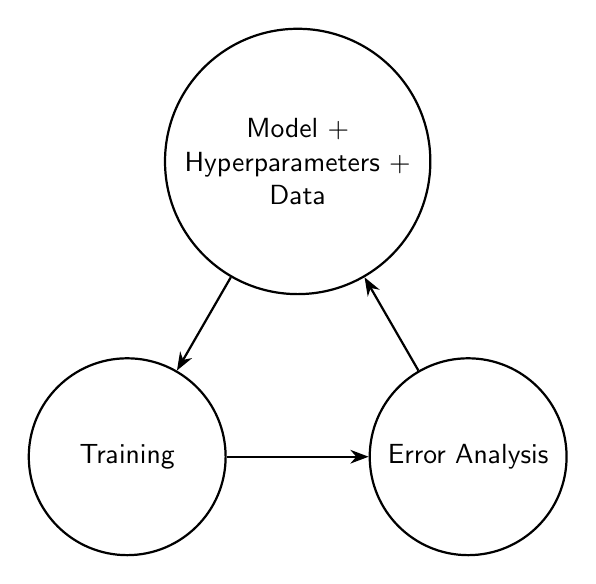
\begin{tikzpicture}[>=Stealth, thick]

% Define the circle nodes
\node[circle, draw, minimum size=2.5cm, align=center] (model) at (90:2.5) {Model + \\ Hyperparameters + \\ Data};
\node[circle, draw, minimum size=2.5cm, align=center] (training) at (210:2.5) {Training};
\node[circle, draw, minimum size=2.5cm, align=center] (error) at (330:2.5) {Error Analysis};

% Add arrows between the nodes
\draw[->, thick] (model) -- (training) node[midway, above left] {};
\draw[->, thick] (training) -- (error) node[midway, below] {};
\draw[->, thick] (error) -- (model) node[midway, above right] {};

\end{tikzpicture}
\caption{An iterative machine learning process. The cycle involves three steps: configuring the model (with hyperparameters and data), training the model, and performing error analysis. Each step informs improvements to the others, ensuring systematic optimization of performance.}
\label{fig:ml_cycle}
\end{figure}



This chapter outlines a systematic approach to diagnosing error gaps—disparities between different error numbers—and applying targeted strategies to address them. These gaps provide insights into the root causes of performance issues, such as avoidable bias, variance, data mismatch, overfitting, or shortcut learning. By leveraging orthogonalization principles, you can efficiently improve your model by isolating each problem and addressing it directly, rather than making broad, unfocused changes. \newline

The process begins with error analysis (section: \ref{sec:error_analysis}), where you examine and quantify the gaps between error metrics, such as Bayes error, training error, and validation error. The gaps all highlight the issues in your workflow, but it all depends on how big the gaps are. The most pressing issues are indicated by the biggest gaps. Once you identify the primary problem (biggest error gap), you can refer to the section "Addressing Sources of Error Gaps" (\ref{sec:addressing_sources_error_gaps}), which is divided into subsections, each containing techniques to address a specific root cause, such as overfitting. \newline

\begin{examplebox}
Suppose your model performs poorly on the test set. Through error analysis, you notice a significant gap between the train- and dev set errors, indicating overfitting (high variance). This means the model is memorizing the training data rather than generalizing. Once you identify overfitting as the primary issue, you can address it with techniques tailored to this problem (found in subsection: \ref{sec:addressing_variance}), such as regularization, adding more training data, or simplifying the model architecture. By targeting overfitting specifically, you make meaningful progress without inadvertently introducing new issues. After implementing these changes, you repeat the cycle: train the model again, perform error analysis, and identify if your modifications resolved the issue or if other problems need to be addressed.
\end{examplebox}


In summary, the key steps are simple: examine error metrics, identify the largest gaps, understand their sources, and apply targeted solutions. This structured approach ensures that every improvement is intentional, measurable, and focused on addressing the most significant problems in your machine learning project.


\section{Error Analysis} \label{sec:error_analysis}

As discussed in the introduction of this chapter, diagnosing the sources of your model’s poor performance begins with a careful examination of error metrics. Error analysis focuses on identifying and quantifying the gaps between different error numbers, such as Bayes error, train- and dev set errors. Each of these metrics represents a specific stage of your workflow, and the gaps between them highlight the root causes of performance issues. \newline

These gaps are not just indicators of where problems exist—they also reveal how significant those problems are. For example, a large gap between training and validation error points to overfitting, where the model performs well on the training data but fails to generalize. By systematically analyzing these gaps, you can pinpoint the biggest obstacles in your workflow and prioritize addressing them. This structured process lays the foundation for targeted solutions, as described in the next section (Addressing Sources of Error Gaps: \ref{sec:addressing_sources_error_gaps}).

\subsection{Overview of Error Numbers and Sources of the Gaps}

Figure ~\ref{fig:error-hierarchy} summarizes the key error numbers encountered during a machine learning project and shows the sources of the gaps between the error numbers:

\begin{figure}[H]
    \centering
    \[
    \begin{array}{r@{\hspace{2em}}c@{\hspace{2em}}l}
        \textbf{(Zero error)} & & \\[1em]
        & \updownarrow & \text{(Unavoidable error)} \\[1em]
        \textbf{Bayes error} & & \\[1em]
        & \updownarrow & \text{Underfitting} \\[1em]
        \textbf{Train set error} & & \\[1em]
        & \updownarrow & \text{Overfitting the train set} \\[1em]
        \textbf{(Train-dev set error)} & & \\[1em]
        & \updownarrow & \text{(Data mismatch)} \\[1em]
        \textbf{Dev set error} & & \\[1em]
        & \updownarrow & \text{Overfitting the dev set} \\[1em]
        \textbf{Test set error} & & \\[1em]
        & \updownarrow & \text{(Shortcut learning)} \\[1em]
        \textbf{(Gen set error)} & & \\
    \end{array}
    \]
    \caption{Overview of the different error numbers in machine learning projects (in bold, on the left) and the sources of the gaps between them (on the right). Terms in brackets are only present in some situations.}
    \label{fig:error-hierarchy}
\end{figure}

\subsubsection{Error Numbers}
Each error number reflects a specific stage in the project and provides information on the performance of the model, or represents a useful theoretical concept that helps to put the model performance into context.
\begin{itemize}
    \item \textbf{Zero Error} The theoretical scenario where the model makes no mistakes. When this is unequal to Bayes error, it is impossible for the model to reliably achieve perfect performance on unseen data.
    \item \hypertarget{bayes-error}{\textbf{Bayes Error:}} The theoretical lower bound on error, determined by the information content of the data itself. This represents the ideal performance of a model, the hard upper bound on performance. The Bayes error can be equal to zero error, but in most cases it is greater due to limitations such as inherent noise or ambiguity in the data. It is theoretically possible for a model to reliably achieve Bayes error on unseen data.
    \item \textbf{Train Set Error:} The error on the training data, which indicates how well the model has fit the train set.
    \item \textbf{Train-Dev Set Error:} The error on an optional train-dev set, sampled from the training distribution but not used for training. This helps to distinguish between the case where the model overfits the train set and data mismatch problems when the train set is coming from a different distribution than the dev set.
    \item \textbf{Dev Set Error:} Informs hyperparameter tuning and serves as a proxy for the test set performance.
    \item \textbf{Test Set Error:} Indicates final model performance on unseen data.
    \item \textbf{Gen Set Error:} The error on the generalization set, which comes from a different distribution than the test set, which however is also relevant for the application (see subsection~\ref{subsec:detecting-shortcut-learning} for explanations).
\end{itemize}

\subsubsection{Sources of the gaps between error numbers}

\begin{itemize}
    \item \textbf{Unavoidable Error:} The gap between zero error and Bayes error, which arises due to intrinsic limitations of the dataset such as noise or ambiguity. This error gap cannot be eliminated.
    \item \textbf{Underfitting:} The gap between Bayes error and the train set error. This gap arises from the model's limitations in capturing the underlying patterns in the data, because it lacks capacity/complexity. The ideal model has a train set error equal to the Bayes error.
    \item \textbf{Overfitting the Train Set:} Happens when the model has too much capacity and starts fitting not only the general patterns in the training data, but also the accidental noise. Since noise is random and not present in the same form in new data, this leads to poor generalization. It is observed as a large gap between train and dev set performance.
    \item \textbf{Data Mismatch:} The gap between the train-dev error and the dev set error, caused by differences in the distributions of the training and dev/test sets.
    \item \textbf{Overfitting the Dev Set:} The gap between the dev set error and the test set error, indicating that the model has overfit to the dev set. This often occurs when hyperparameters are inadvertently tuned to minimize the dev set error through extensive optimization, leading to a model that performs well on the dev set but fails to generalize to unseen test data.
    \item \textbf{Shortcut Learning:} The gap between the test set error and the gen set error. This indicates that the model has learned superficial patterns that do not generalize across relevant distributions.
\end{itemize}


\subsection{Proxy for Bayes Error} \label{subsec:proxy-for-bayes-error}
Since the true Bayes error is unknown, we must use proxies to estimate it:
\begin{itemize}
    \item \textbf{Human-level performance (when applicable):} Often close to Bayes error for tasks humans are skilled at, such as natural perception (e.g. image classification).
    \item \textbf{Other proxies:} For tasks humans are poor at, such as predicting weather patterns or network traffic, alternatives include state-of-the-art model performance, cross-model agreement, or domain-specific insights (e.g., noise levels or uncertainty analysis). 
\end{itemize} 

\begin{notebox}
When using human-level performance as a proxy for Bayes error in classification tasks, ensure that the labels were not originally assigned by a human. If they were, HLP reflects the agreement between two labelers rather than truly approximating Bayes error. In such cases, it indicates ambiguities in the labeling process rather than the irreducible error.
\end{notebox}

\begin{notebox}
When deciding what to use as a proxy for the Bayes error, you should generally choose the one with the lowest error available. By definition, Bayes error is always lower than any observed error, so the proxy with the lowest error will be the closest to the Bayes error and thus the best estimate. 
\end{notebox}

\begin{notebox}
The performance baseline (Section~\ref{sec:performance_baseline}) and the proxy for Bayes error define the lower and upper performance bounds, but their roles can sometimes be confusing, because they are context-dependent. For example, state-of-the-art model performance or human-level performance can act as either a baseline or a proxy, depending on the project’s goals and value proposition. If the value lies in surpassing an existing system (e.g., improving a company’s current model), it serves as the baseline. On the other hand, if the value comes from approaching the performance of an existing standard (e.g., automating a task currently done by humans), it acts as the proxy for Bayes error.
\end{notebox}


\subsection{Under- and Overfitting with Mismatched Data Distributions}
The approach of analysing under- and overfitting changes when the train and dev/test sets come from different distributions. In this scenario, additional techniques are required to pinpoint the source of errors. \newline

To address this issue, introduce a \textbf{train-dev set}: a subset of data that shares the same distribution as the training set but is not used during training. The train-dev set helps separate errors due to overfitting the train set from those caused by distribution mismatch.

\begin{itemize}
    \item \textbf{Overfitting Problem:} If there is a significant gap between the train error and the train-dev error, but the gap between train-dev and dev is small, it indicates the model is overfitting the train set. 
    \item \textbf{Data Mismatch Problem:} If the error difference between the train and train-dev sets is small, but the dev/test error is significantly higher, the issue lies with the data distribution mismatch.
\end{itemize}

\begin{notebox}
Both overfitting the train set and data mismatch problems can occur simultaneously.
\end{notebox}


\subsection{Detecting Overfitting the Dev Set}

Overfitting to the dev set occurs when the model performs well on the dev set but struggles to generalize further. This can happen when the dev set becomes too small or when it is used excessively during hyperparameter tuning. \newline

The degree of overfitting to the dev set can be determined by comparing the dev set error to the test set error:
\[
\text{Degree of Overfitting the Dev Set} = \text{Test Set Error} - \text{Dev Set Error}
\]


\subsection{Detecting Shortcut Learning} \label{subsec:detecting-shortcut-learning}

Shortcut learning occurs when a model learns superficial patterns or correlations in the data that work well for the test set but fail to generalize to other relevant distributions within the same application domain. This can be identified by comparing the performance of the model on the test set and a \textbf{generalization set (gen set)}. \newline

\begin{examplebox}
Lets say there is an image classifier trained to detect sheep. If the training and test images predominantly show sheep in green fields, the model might take a shortcut and learn to associate the presence of a green background with sheep, rather than learning to identify the actual features of the sheep. As a result, the classifier might fail to recognize sheep in a stable or on a rocky hillside, where the green background is absent. This demonstrates how shortcut learning can lead to poor generalization, as the model relies on superficial correlations instead of meaningful features. By evaluating the model on a gen set containing sheep in varied environments, such as stables or rocky landscapes, this limitation can be identified and addressed. 
\end{examplebox}


The \textbf{gen set} represents the same task as the test set but comes from a different distribution, which is still relevant to the application. For instance:
\begin{itemize}
    \item \textbf{Test Set Example:} Blurry cat images taken by amateur photographers from Central Europe, which represents the primary application.
    \item \textbf{Gen Set Example:} Similar blurry cat images, but taken by amateur photographers from India. Although the gen set has a different distribution (different backgrounds, different lighting conditions), it remains relevant to the intended application of classifying user-uploaded photos.
\end{itemize}

The degree of shortcut learning is quantified as the difference between the error on the test set and the error on the gen set:
\[
\text{Degree of Shortcut Learning} = \text{Gen Set Error} - \text{Test Set Error}
\]

A large gap between the gen set error and the test set error indicates that the model may have learned shortcuts that do not generalize well beyond the test set's specific distribution. Detecting and addressing shortcut learning can improve the robustness and applicability of the model in real-world scenarios. \newline

\begin{notebox}
The gen set should not be merged with the test set, as they serve distinct purposes: the test set evaluates performance on the primary application distribution, while the gen set diagnoses robustness and generalization issues, such as shortcut learning. Merging them could dilute these objectives and reduce the diagnostic value of the gen set.
\end{notebox}

\begin{notebox}
Shortcut learning can also be detected by using feature importance algorithms to evaluate whether the model relies on features that are genuinely relevant to the task, rather than superficial or spurious correlations.
\end{notebox}


\subsection{"Higher-Resolution" Error Analysis}

This subsection presents techniques that allow you to delve deeper into the sources of error within one of the five primary categories: avoidable bias, variance, data mismatch, overfitting to the dev set, or shortcut learning. By applying these methods, you can break down errors into finer-grained categories, providing a higher-resolution view of where the model struggles and enabling more targeted and effective improvements.

\subsubsection{Ceiling of Performance Increase}

The ceiling of performance increase is a technique to prioritize efforts by estimating how much error reduction can realistically be achieved by resolving specific problems. This step helps focus resources on the most impactful categories of errors, regardless of whether they arise from bias, variance, or other issues. \newline

The ceiling of performance increase estimates the maximum potential improvement in the overall error if a particular type of error is completely resolved. For example:
\begin{itemize}
    \item If your model's overall error rate is 10\% and only 5\% of this error (so 0.5 \% overall error) comes from incorrectly labeling dogs as cats, fully solving this issue would reduce the error to 9.5\%. This suggests that the effort might not be worthwhile.
    \item Conversely, if 50\% of the error comes from mislabeling dogs as cats (so 5\% overall error), solving this problem could reduce the error to 5\%, making it a much more impactful area to address.
\end{itemize}

To perform this analysis, examine a sample of the model's predictions compared to the ground truth, such as reviewing 100 instances. Split the errors into meaningful categories based on identifiable patterns, such as specific classes, input types, or conditions. Quantify how much each category contributes to the total error, and prioritize addressing the categories that account for the largest share. \newline

As an illustrative example of high-resolution error analysis in speech recognition, consider  predictions of a speech-to-text algorithm. Table~\ref{tab:example_predictions} presents a small selection of dev set instances, showing the ground-truth labels, the algorithm’s predictions, and the presence of specific issues such as car noise, people noise, and low bandwidth. This example demonstrates how noise and other environmental factors can lead to misrecognitions, such as substituting words or phrases with incorrect alternatives. By analyzing these instances, you can identify recurring error patterns in your development set and evaluate how fully resolving these issues could improve the overall performance of the speech recognition system. This helps you in identifying if it is worth the effort.

\begin{table}[ht]
\caption{Example predictions with noise and bandwidth effects.}
\label{tab:example_predictions}
\centering
\resizebox{\textwidth}{!}{%
\begin{tabular}{|c|l|l|c|c|c|}
\hline
\textbf{Instance} & \textbf{Label}                & \textbf{Prediction}          & \textbf{Car noise} & \textbf{People noise} & \textbf{Low bandwidth} \\ \hline
1                & “Stir fried lettuce recipe”   & “Stir fry lettuce recipe”    & 1                  &                      &                       \\ \hline
2                & “Sweetened coffee”            & “Swedish coffee”             &                    & 1                    & 1                     \\ \hline
3                & “Sail away song”              & “Sell away some”             &                    & 1                    &                       \\ \hline
4                & “Let’s catch up”              & “Let’s ketchup”              & 1                  & 1                    & 1                     \\ \hline
\end{tabular}%
}
\end{table}


Systematically estimating the ceiling of performance increase can be more straightforward for natural perception tasks like image classification, where humans are highly skilled at recognizing patterns. For other classification or regression tasks, where human intuition may be less reliable, focus on analyzing the most frequent or impactful errors directly. For classification tasks, group errors by their predicted and true classes, and quantify the contribution of each misclassification type to the overall error (making a confusion matrix). For regression tasks, sort predictions by the largest absolute errors and identify patterns or specific regions where the model struggles, such as outliers or consistent underestimation. These methods help structure the analysis even when human intuition is limited.

\subsubsection{Data Distribution Resolved Error Analysis}

In some machine learning projects, you may consider expanding your training set by including data from outside the dataset that directly targets your application. For instance, you might incorporate general-purpose data for the task that comes from a different distribution. This leads to the presence of two or more distinct data distributions within your project. \newline

To extend the error analysis framework outlined above to account for multiple data distributions, you can resolve the error numbers separately for each distribution. This provides deeper insights into the performance of your model across diverse data sources and helps identify distribution-specific issues. The extended framework, as shown in the table below, provides a structured way to analyze and compare errors across different distributions.

\begin{table}[ht!]
\caption{Extended technique for error analysis to resolve for the different data distributions.}
\label{tab:errors_distributions}
\centering
\resizebox{\textwidth}{!}{%
\begin{tabular}{@{}lccc@{}}
\toprule
\textbf{Metric} & \textbf{Distribution 1} & \textbf{Distribution 2} & \textbf{Distribution 3 \dots} \\ \midrule
Proxy for Bayes error        & Human level 4\%      & Human level 6\%                   & \dots                         \\ 
Error on instances trained on & Train error 7\%      & Train error 6\%                   & \dots                         \\ 
Error on instances not trained on & Train-dev error 10\% & Dev/Test error 6\%    & \dots                         \\ \bottomrule
\end{tabular}%
}
\end{table}


\subsection{Conclusion}
Effective error analysis is a cornerstone of building robust machine learning models. By systematically examining the gaps between different error metrics—such as avoidable bias, variance, data mismatch, overfitting to the dev set, and shortcut learning—practitioners can identify and prioritize the most critical issues affecting model performance. This structured approach ensures that resources are directed toward impactful improvements, enhancing both model generalization and applicability. \newline

For tasks where human intuition may be limited, such as regression or classification tasks with abstract data, techniques like confusion matrices, sorting by absolute errors, and identifying distribution-specific patterns enable deeper insights into model performance. Additionally, extending error analysis to account for multiple data distributions allows for a more nuanced understanding of the model’s strengths and weaknesses across diverse scenarios. \newline

Ultimately, error analysis provides a clear framework for understanding the limitations of a model and guides iterative improvements, helping bridge the gap between current performance and the desired level of accuracy. By incorporating these strategies, machine learning practitioners can build more reliable and generalizable models, driving better outcomes for their applications.


\section{Addressing Sources of the Error Gaps} \label{sec:addressing_sources_error_gaps}

Once error analysis has identified the sources of the gaps between error numbers, the next step is to apply targeted strategies to address the most pronounced problem. This section provides collections of techniques for each type of problem, offering practical methods to reduce avoidable bias, variance, data mismatch, overfitting to the dev set, and shortcut learning.

\subsection{Addressing Underfitting}

Avoidable bias (underfitting) refers to the gap between the proxy for Bayes error and the train set error. Reducing this gap improves the model’s ability to fit the training data. Strategies to address avoidable bias include:

\begin{itemize}
    \item \textbf{Increase model capacity:} Use a larger or more complex model, such as increasing the amount of layers in a neural network or transitioning from linear to polynomial regression.
    \item \textbf{Train for longer:} Extend training time by increasing epochs or iterations to ensure the model learns adequately and converges properly.
    \item \textbf{Improve features or representations:} Engage in feature engineering by adding relevant features or deriving new ones to better capture data intricacies. Alternatively, use pretrained embeddings for a richer representation of the data.
    \item \textbf{Reduce regularization:} For example, lower the strength of L1 or L2 penalties to allow the model greater flexibility to fit the training data.
    \item \textbf{Adjust data preprocessing:} Ensure preprocessing steps retain all meaningful information and avoid discarding important patterns.
\end{itemize}

\begin{notebox}
You should not aim for an error lower than your proxy for Bayes error. Having a lower error indicates overfitting, as your model is fitting noise in the data rather than genuine patterns. Recall that no model can reliably perform better than Bayes error on unseen data. Once your model’s error approaches the proxy for Bayes error, avoid making it more powerful, as further adjustments will likely harm generalization.
\end{notebox}


\subsection{Addressing Overfitting the Train Set} \label{sec:addressing_variance}

Overfitting the train set reflects the model’s inability to generalize to unseen data. To effectively address overfitting, it is important to understand \textbf{why} it occurs. Overfitting can stem from two main causes:

\begin{itemize}
    \item \textbf{Too little data:} When training and dev sets are both small, they represent different random subsamples of the population. Even if the model learns only genuine patterns from the training set, these patterns may not transfer well to the dev set simply because the two samples differ due to sampling variability. This is a problem of statistical inference: small samples are unstable and not representative of the full population. The model isn't necessarily learning noise—it just cannot generalize reliably between mismatched subsets.
    
    \item \textbf{Too much model capacity:} The model is flexible enough to fit not just the true patterns but also noise and spurious correlations in the training data. These don’t generalize to new data and cause performance to degrade on the dev set.
\end{itemize}

Once the cause is understood, appropriate strategies can be applied:

\textbf{If the cause is too little or unrepresentative data:}
\begin{itemize}
    \item \textbf{Increase training data:} Gather more labeled examples to reduce sampling error and make the training distribution more representative of the population.
    \item \textbf{Data augmentation:} Expand the training set by adding modified versions of existing data (e.g., rotations, flips, noise), especially in domains like image and audio, where data collection is expensive.
\end{itemize}

\textbf{If the cause is excessive model capacity:}
\begin{itemize}
    \item \textbf{Simplify the model:} Use a smaller or less expressive model (e.g., shallower trees, fewer neural network layers, or switching to a linear model).
    \item \textbf{Apply regularization:} Techniques like L1/L2 penalties, weight decay, or dropout in neural networks constrain the model's ability to overfit.
    \item \textbf{Use early stopping:} Halt training when dev set performance stops improving to prevent the model from continuing to fit noise.
\end{itemize}

\textbf{General strategies that help in both cases:}
\begin{itemize}
    \item \textbf{Employ cross-validation:} Provides a more robust estimate of generalization and helps in tuning hyperparameters effectively.
    \item \textbf{Ensemble methods:} Combining multiple models (e.g., random forests, boosting) improves robustness without increasing overfitting.
\end{itemize}


\subsection{Addressing Data Mismatch}
\label{subsec:Adressing Data Mismatch}

Data mismatch refers to the gap between the train-dev error and the dev set error, caused by differences in the distributions of the training and dev/test sets. Resolving this issue ensures that the model generalizes effectively to the target application. Below are strategies to address data mismatch, with detailed explanations and considerations.

\subsubsection{Carry Out Manual Error Analysis}

Start by performing manual error analysis to understand the nature of the mismatch between the training and dev/test sets. Carefully examine misclassified examples and compare their characteristics with correctly classified instances. This step provides insights into the discrepancies and guides subsequent actions.

\subsubsection{Collect More Aligned Data}

One of the most effective ways to address data mismatch is to collect additional data that aligns with the dev/test distribution. This may involve:
\begin{itemize}
    \item Gathering new samples from the same application domain.
    \item Curating or filtering existing datasets to ensure they match the target distribution.
\end{itemize}
This approach directly mitigates distributional differences and improves the model’s generalization to the dev/test sets.

\subsubsection{Augment or Synthesize Training Data}

Artificial data synthesis and augmentation allow you to leverage existing datasets by transforming them to better resemble the dev/test distribution. Common methods include:
\begin{itemize}
    \item Simulating data that reflects the characteristics of the dev/test sets.
    \item Applying transformations such as noise addition, cropping, rotation, or other domain-specific augmentations.
\end{itemize}

When using data augmentation, it is crucial to consider the following:
\begin{itemize}
    \item \textbf{Avoid limited augmentation variety:} Ensure that the augmentations cover a diverse range of transformations. Over-reliance on narrow variations can lead to overfitting to the augmentation scheme rather than generalizing to the broader target distribution. For example, augmenting 10,000 hours of speech data with only 1 hour of car noise may cause the model to overfit to the specific car noise patterns rather than learning to handle general noise.
    \item \textbf{Maintain realistic transformations:} Augmentations should accurately represent variations likely to be encountered in the application. Unrealistic augmentations can mislead the model and degrade performance.
\end{itemize}

Diverse and realistic data augmentation helps align the training distribution with the target dev/test distribution while minimizing the risk of overfitting.

\subsubsection{Domain Adaptation}

Domain adaptation techniques are designed to bridge the gap between the training and dev/test distributions. Such gaps can occur when the data used to train the model is not representative of the data it will encounter during evaluation or deployment. These methods include:

\begin{itemize}
    \item \textbf{Feature Alignment:} Align the distributions of the training and test data in the feature space.

    \begin{examplebox}
    Imagine training an image classifier on a dataset of outdoor photos taken in bright daylight, but the test images come from overcast or nighttime settings. A feature alignment technique might adjust the brightness and contrast of the training images to match the lighting conditions of the test set, helping the model learn more transferable features.
    \end{examplebox}

    \item \textbf{Domain-Invariant Representation Learning:} Ensure the model learns features that are robust and applicable across different domains, ignoring domain-specific artifacts.

    \begin{examplebox}
    Consider a sentiment analysis model trained on movie reviews and deployed to analyze product reviews. The model might inadvertently focus on features specific to movie reviews (e.g., references to "actors" or "directors"). Domain-invariant representation learning ensures the model learns general sentiment-related features like "great" or "terrible" that work across both domains.
    \end{examplebox}

    \item \textbf{Adversarial Training:} Use a second "adversary" model during training to explicitly minimize the difference between the training and test domain distributions.

    \begin{examplebox}
    If training data consists of handwritten digits collected on white paper and the test data consists of the same digits on colored backgrounds, an adversarial training approach might introduce a discriminator network to ensure the model cannot distinguish between white and colored backgrounds, forcing it to focus on digit shapes instead.
    \end{examplebox}
    
\end{itemize}

\paragraph{When to Use Domain Adaptation:}

Domain adaptation is particularly useful in situations where:
\begin{itemize}
    \item Collecting additional aligned data (data that matches the dev/test distribution) is not feasible.
    \item The training data is much larger and more diverse than the dev/test sets, making it impractical to retrain the model solely on test-aligned data.
\end{itemize}


\subsubsection{Feature Selection}

Feature selection involves identifying and emphasizing features that generalize well across distributions. Focus on features that are robust and relevant to the dev/test distribution while deprioritizing or excluding those that are overly specific to the training data. This reduces the influence of training-specific biases and enhances generalization.

\subsubsection{Conclusion}

Addressing data mismatch requires a combination of strategies tailored to the nature of the problem. Manual error analysis provides the foundation for understanding the mismatch, while data collection, augmentation, domain adaptation, and feature selection offer practical solutions. When applying augmentation or synthesis, ensure diversity and realism to avoid overfitting to a limited subset of transformations. By systematically addressing data mismatch, you can improve the model’s ability to generalize to the target dev/test distribution.

\subsection{Addressing Overfitting to the Dev Set}

Overfitting to the dev set refers to the gap between the dev set error and the test set error. This happens when the model is excessively tuned to the dev set. Strategies to address overfitting to the dev set include:
\begin{itemize}
    \item \textbf{Increase the size of the dev set:} A larger dev set reduces the risk of overfitting to its specific examples.
    \item \textbf{Use k-fold cross-validation:} This reduces dependence on a single dev set by averaging performance over multiple folds.
    \item \textbf{Minimize dev set tuning:} Limit the number of hyperparameter tuning cycles to avoid overfitting.
    \item \textbf{Expand the test set:} Ensure the test set is large and diverse to provide a robust evaluation.
\end{itemize}

\begin{notebox}
To prevent overfitting to the test set, use this dev to test set comparison sparingly, preferably only at the end of the project for final performance assessment.
\end{notebox}

\subsection{Addressing Shortcut Learning}

Shortcut learning refers to the gap between the test set error and the gen set error, where the model relies on superficial patterns that fail to generalize across relevant distributions. Strategies to address shortcut learning include:
\begin{itemize}
    \item \textbf{Leveraging data from a source domain:} The training set is extended with an additional dataset, the source domain, which is specifically designed to facilitate learning independent representations of fundamental factors. This approach promotes independence across different factors of variation in the learned representations, enabling the model to focus on predictive factors and ignore potential shortcut factors during inference. For example, in a text classification task, a shortcut might occur if the model relies on irrelevant features, such as the presence of specific words, instead of understanding the underlying sentiment or topic. By adding a source domain dataset where the distribution of words is systematically varied but the underlying sentiment or topic remains constant, the model learns to represent linguistic features (like syntax and semantics) independently of spurious correlations. This enables the model to generalize better to unseen text where shortcuts might not hold.
    \item \textbf{Increase train set diversity:} Collect data that covers a wider range of variations relevant to the task.
    \item \textbf{Introduce additional constraints:} Use regularization or loss functions that penalize reliance on superficial shortcut learning patterns.
    \item \textbf{Review feature importance:} Use techniques like SHAP or LIME to identify features the model relies on and verify their validity.
     \item \textbf{Adversarial Sampling:} Identify examples where the model fails and add similar instances to the training set.
     \item \textbf{Feature Regularization:} Penalize models for relying on certain features through techniques like attention masking or saliency regularization.
\end{itemize}



\chapter{Performance Auditing}

Even when a learning algorithm achieves high accuracy, F1-score, or another relevant metric, it is crucial to conduct a final performance audit before deploying it to production. This step can prevent significant post-deployment issues and ensure that the system operates reliably across various conditions. 

\section{Framework for Performance Auditing}

A structured approach to performance auditing involves the following steps:

\subsection{Brainstorm Potential Failure Modes}
Start by identifying possible ways the system might fail. Consider:
\begin{itemize}
    \item \textbf{Subgroup Performance}: Does the model perform consistently across different demographic groups, such as different genders or ethnicities?
    \item \textbf{Error Analysis}: Are false positives or false negatives disproportionately high in certain cases?
    \item \textbf{Rare and Important Cases}: How does the model handle rare but critical classes?
    \item \textbf{Domain-Specific Concerns}: Are there any industry-specific fairness or bias concerns?
\end{itemize}

\subsection{Define Metrics for Evaluation}
Once potential issues are identified, define appropriate metrics to assess them. A common strategy is \textbf{evaluating performance on slices of the data} rather than the entire dataset. For example:
\begin{itemize}
    \item Measure accuracy on specific subgroups (e.g., different demographics, device types, or accent variations in speech recognition systems).
    \item Evaluate fairness metrics such as disparate impact or equalized odds.
    \item Analyze whether error types (false positives vs. false negatives) align with acceptable trade-offs.
\end{itemize}

\subsection{Automate Performance Auditing with MLOps Tools}
Leveraging MLOps tools can streamline the auditing process:
\begin{itemize}
    \item \textbf{TensorFlow Model Analysis (TFMA)}: Computes detailed metrics for different slices of data.
    \item \textbf{Custom Monitoring Pipelines}: Set up automatic triggers for evaluations before deployment.
    \item \textbf{Buy-in from Stakeholders}: Engage business and product teams to ensure that identified concerns align with practical requirements.
\end{itemize}

\subsection{Address Identified Issues}
If any issue is detected, update the model before deployment to mitigate potential risks. Catching problems at this stage is far more efficient than dealing with them post-deployment.

\section{Case Study: Speech Recognition Auditing}
Consider a speech recognition system undergoing performance auditing:
\begin{enumerate}
    \item \textbf{Brainstorming Failures}:
    \begin{itemize}
        \item Performance varies across different genders and accents.
        \item Accuracy differs depending on the microphone quality of different devices.
        \item The system occasionally mistranscribes words into offensive language.
    \end{itemize}
    \item \textbf{Defining Metrics}:
    \begin{itemize}
        \item Measure mean accuracy per gender and accent.
        \item Compare model accuracy across different device types.
        \item Detect and flag mistranscriptions that result in inappropriate language.
    \end{itemize}
    \item \textbf{Addressing Issues}:
    \begin{itemize}
        \item Adjust training data representation to improve fairness.
        \item Implement additional filtering for offensive mistranscriptions.
    \end{itemize}
\end{enumerate}

\section{Industry-Specific Standards \& Team-Based Auditing}
Performance auditing should align with evolving industry standards. The definition of fairness and bias in AI continues to develop, and best practices vary across domains. Teams should:
\begin{itemize}
    \item Regularly review fairness guidelines relevant to their field.
    \item Conduct audits collaboratively to avoid individual bias in identifying potential failures.
    \item Seek external advisors for additional perspectives on high-stakes applications.
\end{itemize}

\section{Conclusion}
By proactively auditing performance, teams can deploy machine learning models with greater confidence. A well-audited system reduces the risk of unintended consequences, ensuring robustness, fairness, and reliability in production environments.




\part{Insights}


\chapter{Introduction to Insight Extraction}

\begin{summarybox}
\begin{itemize}
  \item Insight extraction transforms a model from a black box into a tool for strategy and decision-making.
  \item Use it when prediction is not the final goal, or when actionability and explainability are important.
\end{itemize}
\end{summarybox}

\section{Purpose of this Stage}

The insight extraction stage exists to answer one core question: \textbf{What can we learn from this model that helps us make better decisions?} While the modeling stage focuses on optimizing predictive performance, insight extraction focuses on translating that model into understanding, strategy, or intervention. This step is essential when the end goal is not automation, but human decision-making.

\begin{notebox}
Insight extraction is often where the actual business value gets realized — especially in settings where the model is never deployed.
\end{notebox}

\section{Why Insights are unequal to Prediction}

Predictive models tell us \emph{what is likely to happen}. Insights tell us \emph{why it is happening}, and more importantly, \emph{what we can do about it}. A high-performing model is not automatically insightful — it may rely on spurious correlations, use non-actionable variables, or behave unpredictably under intervention.

\begin{examplebox}
A model might predict customer churn with 90\% AUC using features like zip code or age. This helps you flag risk but offers no guidance for retention strategies, because these features can’t be changed.
\end{examplebox}

To extract insight, you need to go beyond performance metrics and investigate how the model reaches decisions, which features it responds to, and what hypothetical changes might alter its outputs.

\section{When to Prioritize Insights Over Deployment}

Insight extraction should be prioritized when:
\begin{itemize}
  \item The business problem is exploratory or strategic in nature (e.g., ``Why are users dropping off?'')
  \item You cannot or do not intend to deploy a model
  \item Interventions require understanding, not just prediction
  \item Stakeholders demand explainability for trust, compliance, or governance reasons
\end{itemize}

\begin{examplebox}
A company wants to understand what drives loan defaults, not just predict them. They plan to adjust approval criteria, change onboarding processes, and redesign communication. A black-box model may be accurate but useless without insight into its internal logic.
\end{examplebox}



\chapter{Global Model Interpretation}

Global model interpretation aims to answer: \textbf{What patterns has the model learned across the entire dataset?} This type of analysis helps you understand overall trends, identify influential features, and extract high-level rules. It is useful when the objective is to inform strategic decisions or communicate findings to non-technical stakeholders.


\begin{summarybox}
\begin{itemize}
  \item Use global interpretation to understand overall model behavior and trends.
  \item Feature importance shows what matters; PDP and SHAP reveal how it matters.
  \item Surrogate models offer simplified rule sets for communicating complex logic.
\end{itemize}
\end{summarybox}

\section{Feature Importance}

Feature importance is the process of identifying which features most influence the model’s predictions. It answers the question: \textit{What is the model paying attention to?}

This insight is essential for validating model behavior, communicating findings, and guiding follow-up actions. Importance scores can be computed in different ways, depending on the model type and your need for interpretability, speed, or theoretical rigor.

\subsection{Types of Feature Importance}

There are two broad approaches:

\begin{itemize}
    \item \textbf{Model-Specific Importance:} Uses the internal structure of the model to compute importance. Fast, but potentially biased or inconsistent across models.
    \item \textbf{Model-Agnostic Importance:} Measures how predictions change when a feature is altered. More general, but often slower and sensitive to correlations.
\end{itemize}

\subsection{Common Techniques}

\begin{itemize}
    \item \textbf{Gain-Based Importance:} Used in tree-based models. Ranks features by how much they reduce loss (e.g., Gini or log-loss) when used in splits.
    \item \textbf{Permutation Importance:} Measures the drop in model performance when a feature’s values are randomly shuffled. General and model-agnostic.
    \item \textbf{SHAP Values:} Compute each feature’s contribution to a specific prediction using game theory principles. Aggregating SHAP values across samples yields global feature importance.
\end{itemize}

\begin{notebox}
Gain-based importance is fast but biased toward high-cardinality or continuous features. Permutation importance is more general but sensitive to correlated inputs. SHAP is slower but provides consistent, local-to-global attributions and works across model types.
\end{notebox}

\begin{examplebox}
In a customer churn model, gain-based importance may rank ``account age'' highly because it's frequently used in tree splits. But SHAP values might show that ``number of support tickets'' actually has more influence on individual churn predictions — and better reflects causal intuition.
\end{examplebox}

\subsection{SHAP Plots for Global Insight}

SHAP goes beyond simple rankings by visualizing how feature values relate to their impact on predictions:

\begin{itemize}
  \item \textbf{SHAP Summary Plot:} Combines feature importance, value direction, and feature distribution across the dataset.
  \item \textbf{SHAP Dependence Plot:} Shows how a single feature’s value affects its SHAP value (i.e., contribution), often revealing interactions.
\end{itemize}

\begin{examplebox}
In a fraud detection model, a SHAP summary plot might show that ``transaction amount'' has a non-linear effect: very low and very high values increase risk, while mid-range values are benign. A dependence plot could further show interaction with ``transaction time''.
\end{examplebox}


Figure~\ref{fig:shap-summary-dependence} illustrates two global SHAP visualizations. The summary plot (left) ranks features by overall importance and shows how feature values relate to prediction direction. The dependence plot (right) focuses on a single feature—\textit{AveRooms}—and shows how its value affects model output, capturing potential non-linear effects or interactions.

\begin{figure}[H]
    \centering
    \includegraphics[width=0.9\textwidth]{insights_figures/shap_summary_dependence.png}
    \caption{SHAP summary plot (left) and SHAP dependence plot (right) for a gradient boosting model trained on the California Housing dataset. These plots highlight which features matter most and how specific values influence predictions.}
    \label{fig:shap-summary-dependence}
\end{figure}




\section{Partial Dependence Plots }

Partial Dependence Plots (PDP) show how the model's prediction changes when you vary a feature, holding all others constant. They reveal:
\begin{itemize}
  \item Directionality: Does increasing the feature raise or lower the prediction?
  \item Saturation points or thresholds
  \item Linear vs. nonlinear behavior
\end{itemize}

\begin{notebox}
PDPs assume feature independence, so they're less reliable when features are strongly correlated.
\end{notebox}

Figure~\ref{fig:partial-dependence} shows a partial dependence plot created using a gradient boosting regressor trained on the California Housing dataset. It illustrates how predicted house value changes as the average number of rooms is varied, while all other features are held constant.


\begin{figure}[H]
    \centering
    \includegraphics[width=0.7\textwidth]{insights_figures/partial_dependence_plot.png}
    \caption{Example of a Partial Dependence Plot showing how predicted house value varies with the average number of rooms.}
    \label{fig:partial-dependence}
\end{figure}


\section{Surrogate Models}

Surrogate models are interpretable models (e.g., decision trees or linear models) trained to mimic the behavior of a more complex model. They are not used for prediction themselves — their purpose is to approximate the black-box model’s output in a simplified form that humans can understand.

Use surrogate models when:
\begin{itemize}
  \item You need a simple, rule-based explanation of a complex model’s logic.
  \item You want to extract transparent decision policies from an opaque system.
  \item Stakeholders require interpretable justifications for compliance or trust.
\end{itemize}

\textbf{Why not just train the simple model directly?} Because surrogate models let you \textit{separate performance from interpretability}. You can first train a high-performance black-box model (e.g., a gradient boosting machine or neural network), then fit a simpler model on its predictions to approximate its behavior. This gives you both predictive power and a human-readable explanation — though always approximate.

\begin{examplebox}
A surrogate decision tree might reveal that a fraud model mostly splits based on ``IP mismatch'' and ``unusual login time'', providing a high-level heuristic usable in rule-based systems.
\end{examplebox}




\chapter{Local Model Interpretation}

Local model interpretation focuses on individual predictions. The goal is to understand \textbf{why the model made this specific decision} — which features pushed it in which direction, and whether that outcome could have been different. This is crucial when decisions affect real people (e.g., credit scoring, rejections, medical predictions), or when you need to investigate edge cases, errors, or inconsistencies.

\section{SHAP Force Plots \& Waterfall Plots}

SHAP can break down a single prediction into additive feature contributions:
\begin{itemize}
  \item \textbf{Force plots} visualize how each feature pushes the prediction higher or lower, starting from a base value (the average prediction).
  \item \textbf{Waterfall plots} show the same information, but in a bar-chart-like cumulative form.
\end{itemize}

Use this when:
\begin{itemize}
  \item You need a clear, instance-specific explanation
  \item You want to communicate a decision rationale
  \item Auditing or debugging specific outcomes
\end{itemize}

\begin{examplebox}
A force plot might show that a customer was predicted to churn mainly because of ``low engagement score'' and ``no recent purchases,'' which together outweighed their ``long tenure''.
\end{examplebox}

Figure~\ref{fig:shap-force} and Figure~\ref{fig:shap-waterfall} show two ways to explain a single model prediction using SHAP. The force plot highlights how each feature pushes the prediction above or below the average baseline, while the waterfall plot presents the same contributions in a bar-style format. Both are useful for auditing, debugging, and communicating individual decisions.

\begin{figure}[H]
    \centering
    \includegraphics[width=0.85\textwidth]{insights_figures/shap_force_plot.png}
    \caption{SHAP force plot showing how each feature contributes to a single prediction. The model starts at the average prediction and adjusts based on each feature’s SHAP value.}
    \label{fig:shap-force}
\end{figure}

\begin{figure}[H]
    \centering
    \includegraphics[width=0.75\textwidth]{insights_figures/shap_waterfall.png}
    \caption{SHAP waterfall plot presenting the same prediction explanation in a cumulative bar chart, sorted by feature impact.}
    \label{fig:shap-waterfall}
\end{figure}




\section{LIME}

LIME (Local Interpretable Model-agnostic Explanations) fits a simple interpretable model (like a linear model) around a single prediction by sampling nearby data points. It’s model-agnostic and especially useful for non-tree models like neural nets or ensembles.

Use LIME when:
\begin{itemize}
  \item You can’t use SHAP (e.g., unsupported model)
  \item You want a simple explanation with coefficients
  \item You’re working with tabular, text, or image data
\end{itemize}

\begin{notebox}
LIME’s outputs can be unstable and sensitive to how it samples the neighborhood, so don’t overtrust it without sanity checks.
\end{notebox}

\begin{examplebox}
For a customer with a predicted loan rejection, LIME might show that the main drivers were ``unstable income'' and ``high debt-to-income ratio'', with weights derived from the local linear fit.
\end{examplebox}

\section{Counterfactual Explanations}

Counterfactuals answer the question: \textbf{What minimal change would have led to a different prediction?} Unlike SHAP or LIME, this is not about explaining what happened — it’s about showing how to achieve a different outcome.

Use counterfactuals when:
\begin{itemize}
  \item You want to identify actionable levers (e.g., ``what would have made this customer stay?'')
  \item You're building decision support tools
  \item You want to test model sensitivity to change
\end{itemize}

\begin{examplebox}
A counterfactual for a rejected loan applicant might say: ``If monthly income were \$300 higher and credit utilization 10\% lower, the loan would have been approved.''
\end{examplebox}

\section{Individual Conditional Expectation (ICE)}

ICE plots show how the prediction for a \textbf{single instance} changes as you vary one feature, keeping the others fixed. Unlike PDPs (which average across all instances), ICE focuses on local sensitivity.

Use ICE plots to:
\begin{itemize}
  \item Explore how sensitive a prediction is to a specific feature
  \item Investigate edge cases
  \item Find interaction effects (by comparing ICE curves across many instances)
\end{itemize}

\noindent\begin{minipage}{\textwidth}
\begin{notebox}
ICE assumes features can be changed independently, which may not hold if inputs are correlated or constrained.
\end{notebox}
\end{minipage}

\begin{examplebox}
For one user, an ICE plot might show that increasing ``app visits per week'' linearly reduces churn probability — useful for designing retention strategies.
\end{examplebox}

\begin{summarybox}
\begin{itemize}
  \item Local interpretation explains why a specific prediction happened.
  \item SHAP force plots are best for additive, consistent explanations.
  \item LIME provides interpretable approximations for complex models.
  \item Counterfactuals highlight what could have changed the outcome.
  \item ICE plots show local sensitivity to feature changes.
\end{itemize}
\end{summarybox}




\chapter{Behavioral and Segment Analysis}

Behavioral and segment analysis focuses on identifying meaningful subgroups within your data — and understanding how model behavior or feature effects differ across these groups. Instead of treating the population as homogeneous, you deliberately seek heterogeneity in feature importance, relationships, and outcomes. This is essential when your users, products, or cases fall into qualitatively different categories that require different strategies.

\section{Clustering Post-Modeling}

Clustering after model training can reveal behavioral patterns or user segments that relate to the prediction in different ways. You cluster based on either:
\begin{itemize}
  \item Original features (behavioral segmentation)
  \item SHAP values or model outputs (model-behavior segmentation)
\end{itemize}

\begin{examplebox}
You may find a cluster of users with low predicted churn, but high actual churn. Investigating this group could reveal missing behavioral signals or a need for a specialized retention strategy.
\end{examplebox}

Use clustering to:
\begin{itemize}
  \item Discover overlooked user types
  \item Identify outlier groups for targeted analysis
  \item Visualize behavior patterns in reduced-dimensionality plots (e.g., UMAP or t-SNE on SHAP)
\end{itemize}

\section{Subgroup-Specific Feature Effects}

Not all features affect all users equally. After identifying clusters or known subgroups (e.g., age groups, product tiers), examine whether feature effects differ between them. This can be done via:
\begin{itemize}
  \item Stratified SHAP summary plots
  \item Separate PDP or ICE plots per group
  \item Training interpretable models on each subgroup
\end{itemize}

\begin{examplebox}
For premium users, ``response time from support'' may be a strong churn driver, while for freemium users it barely matters. Separate SHAP plots can reveal this difference clearly.
\end{examplebox}

This type of analysis is critical when:
\begin{itemize}
  \item Designing differentiated product strategies
  \item Building segment-aware intervention plans
  \item Evaluating fairness and bias
\end{itemize}

\section{Interaction Effects and Heterogeneity}

Models often learn that combinations of features matter more than any feature alone. Global feature importance won’t detect this — you need to explore interactions directly.

Tools to uncover interaction effects include:
\begin{itemize}
  \item SHAP interaction values (tree-based models only)
  \item PDPs or ICE plots with a second feature overlay
  \item Two-way ALE plots (Accumulated Local Effects)
\end{itemize}

\begin{notebox}
Strong interaction effects often indicate that a single global policy won't work. Segment-specific decisions become necessary.
\end{notebox}

\begin{examplebox}
An interaction effect may show that ``discount offers'' reduce churn only for users with low engagement scores — offering discounts to active users has no effect.
\end{examplebox}

\begin{summarybox}
\begin{itemize}
  \item Segment analysis reveals patterns missed by global interpretation.
  \item Cluster users post-modeling to identify strategic subgroups.
  \item Check whether feature effects differ across known or discovered groups.
  \item Use interaction analysis to uncover conditional dependencies that affect actionability.
\end{itemize}
\end{summarybox}




\chapter{Simulation and Scenario Testing}

A trained model doesn’t have to be deployed to be useful. It can also serve as a simulation tool: a way to test hypothetical scenarios, estimate impacts, and support better decision-making. This is especially valuable in environments where experimentation is expensive or risky, and where you want to explore possible interventions before implementing them.

\section{What-If Analysis}

What-if analysis involves modifying input features and observing how the model prediction changes. It answers questions like:
\begin{itemize}
  \item What happens if we increase feature X?
  \item How sensitive is the outcome to this variable?
  \item Does this intervention reduce risk, cost, or likelihood of churn?
\end{itemize}

\begin{examplebox}
A retention team might simulate a 10\% increase in app engagement across all users and observe how many drop from ``high churn risk'' to ``medium''. This can help prioritize product updates or outreach.
\end{examplebox}

What-if analysis works best when:
\begin{itemize}
  \item You have clear intervention levers (e.g., pricing, service frequency)
  \item You're comparing competing business actions
  \item You're building decision-support tools, not automation
\end{itemize}

\section{Using Models for Virtual Experiments}

Instead of deploying a policy and waiting for results, use your model to run “virtual experiments” on historical or synthetic data. You simulate what the model would predict under different inputs, to evaluate:
\begin{itemize}
  \item Likely outcome shifts (e.g., conversion rate, risk level)
  \item Expected gains vs costs
  \item Group-specific effects (e.g., does the change help everyone equally?)
\end{itemize}

\begin{examplebox}
A marketing team simulates the effect of sending promotional emails to different user segments and finds that only low-engagement users show a meaningful uplift in predicted purchase probability.
\end{examplebox}

\begin{notebox}
This does not replace A/B testing — but it helps narrow down which interventions are worth testing in the first place.
\end{notebox}

\section{Visualizing Marginal Effects}

To communicate simulation results, use:
\begin{itemize}
  \item Line plots or heatmaps showing how predicted outcomes change with one or two features
  \item Waterfall plots of expected impact across segments
  \item Bar charts comparing scenarios: current vs hypothetical
\end{itemize}

\begin{examplebox}
A marginal effect plot may reveal that increasing delivery frequency from once to twice per week yields a steep drop in churn, but further increases bring diminishing returns — useful for logistics planning.
\end{examplebox}

\begin{summarybox}
\begin{itemize}
  \item Use your model as a sandbox to simulate decisions and explore consequences.
  \item What-if analysis helps evaluate individual or aggregate interventions.
  \item Virtual experiments support prioritization before launching real-world changes.
  \item Visualizations make simulated impacts easier to communicate and justify.
\end{itemize}
\end{summarybox}




\chapter{Causal Thinking and Business Relevance}

Accurate predictions are not enough when the goal is to influence outcomes. In many business settings, the real question is not \textit{who is at risk}, but \textit{what can we change to reduce that risk}. This is where causal thinking becomes essential. Without it, you risk making decisions based on spurious correlations or changing variables that don't actually drive outcomes.

\section{Actionability vs Correlation}

Just because a feature is important to the model doesn't mean it's actionable. Age, geography, or past behavior may be highly predictive — but you can’t change them. Worse, you might misinterpret correlation as leverage for intervention.

\begin{examplebox}
A model may show that users with high browsing time are less likely to churn. But trying to increase browsing time directly (e.g., via forced engagement popups) might not reduce churn — it could just annoy users — because browsing time is a symptom, not a cause.
\end{examplebox}

Causal thinking forces you to ask: \textbf{If we intervene on this feature, will it change the outcome?}

\section{Causal Inference from Observational Data}

While randomized controlled trials (RCTs) are the gold standard, they’re often impractical. Fortunately, there are tools that help estimate causal effects from existing data:
\begin{itemize}
  \item \textbf{Propensity Score Matching:} Balances treated and untreated groups to mimic randomization.
  \item \textbf{Uplift Modeling:} Estimates the differential impact of an intervention.
  \item \textbf{DoWhy or CausalML libraries:} Automate common causal inference workflows.
\end{itemize}

Use causal inference tools when:
\begin{itemize}
  \item You want to quantify the effect of a treatment (e.g., promo, support call, UI change)
  \item You’re making policy or product decisions
  \item You can’t run A/B tests but still need actionable estimates
\end{itemize}

\begin{notebox}
Always sanity-check your assumptions — causal inference from observational data is fragile without domain knowledge.
\end{notebox}

\section{Estimating Treatment Effects}

Causal methods allow you to estimate:
\begin{itemize}
  \item \textbf{Average Treatment Effect (ATE):} What is the expected benefit of this intervention?
  \item \textbf{Conditional Treatment Effect (CATE):} What is the benefit for a specific subgroup?
  \item \textbf{Individual Treatment Effect (ITE):} What would happen to this individual if we intervened?
\end{itemize}

\begin{examplebox}
A telecom company finds that offering a retention bonus reduces churn by 15\% on average (ATE), but only 5\% among long-tenured customers (CATE). This insight helps them avoid wasting budget on the wrong users.
\end{examplebox}

\section{From Insight to Strategy}

Causal insight bridges the gap between analytics and action. Once you know what works, and for whom, you can:
\begin{itemize}
  \item Prioritize interventions with high expected payoff
  \item Avoid strategies based on misleading correlations
  \item Design smarter, more targeted experiments
\end{itemize}

\begin{summarybox}
\begin{itemize}
  \item Correlation is not enough — only causal insight reveals what actually drives change.
  \item Use causal inference tools when you can’t run experiments but need to support decisions.
  \item Estimate treatment effects at the average, segment, or individual level to optimize actions.
  \item Without causal reasoning, business decisions risk wasting resources on false signals.
\end{itemize}
\end{summarybox}



\chapter{Communicating Insights}

Even the most valuable insight is worthless if it isn’t understood or acted upon. Communicating insights means translating complex model behavior into language, visuals, and narratives that stakeholders can use to make decisions. This is not optional — it’s where your work becomes useful.

\section{Translating Model Outputs into Strategy}

Your goal isn’t to impress stakeholders with technical metrics — it’s to answer their questions:
\begin{itemize}
  \item What’s driving this outcome?
  \item What should we do differently?
  \item What trade-offs are we facing?
\end{itemize}

\begin{examplebox}
Instead of presenting “SHAP values and ICE curves,” tell your audience: “High-value users are churning due to poor mobile performance — a 20\% improvement in app speed could reduce churn by 12\% among this group.”
\end{examplebox}

Make it clear what the insight means, who it applies to, and what should change because of it.

\section{Visual Storytelling for Non-Technical Stakeholders}

Don’t overload stakeholders with raw plots. Instead:
\begin{itemize}
  \item Use simple visuals (bar charts, waterfall plots, annotated curves)
  \item Highlight thresholds, changes, and levers
  \item Use color and layout intentionally to guide focus
\end{itemize}

\begin{notebox}
Every plot should answer a specific question — if it doesn’t, leave it out.
\end{notebox}

\begin{examplebox}
A PDP showing diminishing returns on discount level should be annotated with “Optimal range: 10–20\% — above this, additional spend has little effect.”
\end{examplebox}

\section{Prioritizing Interpretability}

Some models are too complex to explain clearly. If interpretability is a priority, consider:
\begin{itemize}
  \item Using simpler models (e.g., shallow trees, logistic regression)
  \item Training interpretable surrogates for communication
  \item Aggregating local explanations into understandable rules
\end{itemize}

\begin{examplebox}
Instead of showing a black-box prediction, present a surrogate rule: “Users are likely to churn if their support rating < 3 and usage dropped > 30\% in the last month.”
\end{examplebox}

\section{Tailoring Insights to Your Audience}

Different stakeholders need different levels of detail:
\begin{itemize}
  \item Executives want trade-offs, outcomes, and decisions
  \item Product teams want user behavior and leverage points
  \item Analysts want clarity and reproducibility
\end{itemize}

\begin{notebox}
Avoid one-size-fits-all reporting. One insight may need multiple presentations.
\end{notebox}

\begin{summarybox}
\begin{itemize}
  \item The value of an insight depends on how well it’s communicated.
  \item Use simple, purpose-driven visuals — not technical plots for their own sake.
  \item Translate model behavior into strategy, not jargon.
  \item Choose explanations your audience can act on — even if it means simplifying.
\end{itemize}
\end{summarybox}



\chapter{Common Pitfalls}

Insight extraction is where real business value can emerge — but it’s also where false confidence and bad decisions are easily introduced. This chapter highlights common mistakes to avoid when interpreting, simulating, or communicating model insights.

\section{Mistaking Correlation for Causation}

This is the most dangerous error. Just because a feature strongly influences predictions does not mean it causes the outcome. Acting on spurious correlations can backfire.

\begin{examplebox}
If high activity predicts low churn, it doesn’t follow that forcing users to be active (e.g., through spammy notifications) will reduce churn — activity may just be a symptom of satisfaction, not a driver.
\end{examplebox}

\section{Overtrusting Feature Importance}

Feature importance methods are often treated as truth, but they:
\begin{itemize}
  \item Are sensitive to correlated features
  \item May reflect model bias, not true signal
  \item Don’t indicate whether features are actionable
\end{itemize}

\begin{notebox}
Always pair feature importance with domain knowledge and context — never treat it as a definitive ranking.
\end{notebox}

\section{Ignoring Unchangeable Features}

A feature may be highly predictive but totally useless for decision-making if it can’t be changed. Age, country, or account creation date might improve model accuracy but provide zero actionable leverage.

\begin{examplebox}
If “signup year” is the top feature in your churn model, your insight is: old users are loyal. That’s nice — but not something you can influence.
\end{examplebox}

\section{Forgetting Segments and Interactions}

Relying only on global explanations hides important heterogeneity. If you fail to analyze subgroups or interactions, you risk building one-size-fits-none strategies.

\begin{notebox}
What works for one user segment might harm another. Always look for diverging patterns.
\end{notebox}

\section{Presenting Without Purpose}

Insights that don’t lead to decisions are just noise. Dumping SHAP plots, PDPs, or ICE curves into a presentation without context or recommendation is a waste of stakeholder time.

\begin{examplebox}
Instead of showing “this feature matters,” aim to say: “This feature matters, and here’s what we should change as a result.”
\end{examplebox}

\begin{summarybox}
\begin{itemize}
  \item Correlation isn’t causation — avoid naive interventions.
  \item Feature importance unequal actionability — don’t confuse influence with leverage.
  \item Always consider heterogeneity and segment-level differences.
  \item Present insights with a clear purpose and actionable next step.
  \item Never turn interpretation into a reporting ritual — it should serve decisions, not decorate slides.
\end{itemize}
\end{summarybox}



\section{Interpreting a Poorly Performing Model}

Even if your goal is not prediction but insight—e.g., understanding feature importance or behavior patterns—model performance still matters. A model that fails to generalize or gets many examples wrong is not a reliable basis for interpretation.

If the model consistently misclassifies or poorly fits the data, any conclusions drawn from it (e.g., which features are most important) are likely misleading. You're interpreting the behavior of a bad model—not the underlying system. At best, the insights are noisy; at worst, they're wrong.

Poor performance is not just an inconvenience—it’s a red flag that the model has not captured the structure you hoped to interpret.

\begin{examplebox}
In a customer churn project, a team used SHAP values from a poorly performing model to draw insights about churn drivers. However, the model barely predicted better than chance—its explanations highlighted noise, not signal. After retraining with proper preprocessing and feature selection, a stronger model revealed completely different and more plausible drivers.
\end{examplebox}





\part{Deployment}

\chapter{Data and Concept Drift}

Deploying a machine learning system is an exciting milestone, but it also introduces a new set of challenges that extend far beyond model training. One of the most significant issues that arise after deployment is the risk of \textbf{data drift} and \textbf{concept drift}. Those are situations where the data distribution or the target relationships shift over time. Addressing these drifts is crucial to maintaining model performance and reliability in real-world applications.

\section{Understanding Data and Concept Drift}

When a machine learning model is trained, it assumes that the data distribution seen during training will remain stable in deployment. However, in most real-world applications, this assumption does not hold. Data evolves due to external factors such as user behavior changes, technological advancements, or economic shifts. The two primary types of drift are data and concept drift. Both types of drift can degrade model performance over time, making continuous monitoring and adaptation essential.

\subsection{Data Drift}

This occurs when the distribution of input features (\(X\)) changes over time, even if the relationship between \(X\) and \(Y\) remains the same. 

\begin{examplebox}
    In a speech recognition system, a new smartphone model with a different microphone can cause shifts in the acoustic data collected.
\end{examplebox}

\begin{examplebox}
    For manufacturing inspection, a visual defect detection model trained under a specific lighting setup may fail if the lighting in the factory changes, altering the image distribution.
\end{examplebox}

\subsection{Concept Drift}

This happens when the underlying relationship between \(X\) and \(Y\) changes, meaning that the same input data no longer maps to the same output labels.
    
\begin{examplebox}
     In fraud detection, before COVID-19, an online shopping pattern with frequent purchases could indicate fraud, but after the pandemic, the same pattern might be considered normal for many users and should not flag those transaction as potential fraud.
\end{examplebox}

\begin{examplebox}
     If a model is trained to estimate house prices based on historical data, an economic shift or inflation could cause significant changes in prices. Here, house sizes (\(X\)) might remain stable, but the target price (\(Y\)) increases, which is a concept drift.
\end{examplebox}

\section{Gradual vs. Sudden Drift}

\textbf{Gradual Drift}: Some changes happen slowly over time, making them less noticeable until they accumulate enough to affect performance. For example, in speech recognition, language evolves as new slang and phrases are introduced gradually. \newline

\textbf{Sudden Drift}: Some shifts occur abruptly, causing an immediate drop in model accuracy. The COVID-19 pandemic triggered such a shift in credit card fraud detection models, as user behaviors changed overnight, making past fraud indicators unreliable.

\section{Detecting Data and Concept Drift}

Monitoring deployed models for drift requires robust detection mechanisms. Some common strategies include:

\begin{itemize}
    \item \textbf{Statistical Tests}: Use statistical methods such as Kolmogorov-Smirnov tests or Population Stability Index (PSI) to compare current input distributions against historical training data.
    \item \textbf{Performance Monitoring}: Track key model metrics like accuracy, precision, and recall over time to detect any sudden drops in performance.
    \item \textbf{Shadow Models}: Deploy a new version of the model alongside the existing one and compare their predictions to detect inconsistencies.
    \item \textbf{Data Sampling}: Continuously collect and analyze recent real-world data to check for discrepancies from the original distribution.
\end{itemize}

\section{Mitigating Drift in Production}

Once drift is detected, appropriate corrective measures must be taken to maintain model performance. Some key approaches include:

\subsection{Retraining Models Regularly}
Periodically retraining the model with fresh data ensures it adapts to changes in data distribution. The retraining frequency depends on how dynamic the data is.

\subsection{Adaptive Learning Approaches}
Techniques such as online learning and continual learning allow models to update incrementally without full retraining. These approaches are particularly useful in rapidly changing environments like financial markets.

\subsection{Feature Engineering Adjustments}
If data drift is detected, new features that better capture the evolving patterns may help restore model accuracy without a full retraining cycle.

\subsection{Hybrid Deployment Strategies}
Deploying multiple models—such as an ensemble of older and newer models—can provide a safety net during data transitions. When significant drift is detected, fallback models can maintain reliability while the primary model is updated.

\section{Key Takeaways}

\begin{itemize}
    \item Data and concept drift are inevitable in most real-world machine learning applications.
    \item Continuous monitoring and statistical methods are essential for detecting drift early.
    \item Effective mitigation strategies include retraining, adaptive learning, and deploying hybrid models.
    \item Proactive drift management helps maintain model reliability and long-term success.
\end{itemize}


\chapter{Deployment Patterns}

Deploying a machine learning model is not simply a matter of turning it on and hoping for the best. There are several strategies to ensure a smooth deployment while minimizing risks. In general, deployment scenarios fall into three broad categories:

\begin{itemize}
    \item Deploying a new product or capability.
    \item Replacing a human-performed task with a learning algorithm.
    \item Updating an existing machine learning system with an improved version.
\end{itemize}

In all these cases, a gradual ramp-up with monitoring is advisable. This allows for performance validation before full-scale deployment. Additionally, rollback mechanisms should be in place in case the new model does not perform as expected.

\section{Shadow Mode Deployment}

A \textbf{shadow mode deployment} allows a new machine learning model to run in parallel with an existing system without affecting real decisions. This is particularly useful when replacing human inspectors or an older machine learning model, as it allows direct comparison of outputs.

\begin{examplebox}
   A smartphone manufacturing plant currently relies on human inspectors to detect scratches on devices. To integrate an AI-based inspection system, a shadow mode deployment is used. The AI model runs alongside human inspectors, generating predictions without influencing factory decisions. If the AI model consistently aligns with human judgments, it can later take on a more active role.
\end{examplebox}

By analyzing discrepancies between human and AI predictions, developers can refine the model before it is entrusted with decision-making.

\section{Canary Deployment}

A \textbf{canary deployment} involves rolling out a new model to a small percentage of real traffic before gradually expanding its reach. This minimizes risks by limiting the impact of potential failures.

\begin{examplebox}
   A defect detection model in a smartphone factory is deployed to inspect only 5\% of production initially. If its performance matches expectations, the deployment is incrementally expanded. In case of errors, rollback is straightforward since most production still relies on the previous system.
\end{examplebox}

This approach helps catch issues early and ensures that any mistakes affect only a small fraction of cases.

\section{Blue-Green Deployment}

A \textbf{blue-green deployment} is used to transition from an old model (blue) to a new model (green) with minimal disruption. Traffic is routed to the blue model initially and switched to the green model when ready.

\begin{examplebox}
   A visual inspection system processes images from factory cameras. Initially, all traffic is routed to the old system (blue). Once the new system (green) is ready, traffic is switched over instantly. If problems arise, the router can redirect traffic back to the blue system.
\end{examplebox}

This method ensures seamless transitions while maintaining the option for rollback.

\section{Choosing the Right Degree of Automation}

Deployment is not a binary decision between manual and fully automated systems. Instead, a spectrum of automation levels exists:

\begin{itemize}
    \item \textbf{Shadow mode}: AI makes predictions but does not influence decisions.
    \item \textbf{AI assistance}: AI highlights areas of interest but does not decide.
    \item \textbf{Partial automation}: AI handles easy cases, while humans review ambiguous ones.
    \item \textbf{Full automation}: AI makes all decisions.
\end{itemize}

\begin{examplebox}
   In a factory setting, an AI system assists inspectors by highlighting possible defects on smartphone screens. This helps inspectors focus on relevant areas, reducing their workload while retaining human oversight.
\end{examplebox}

Many industrial applications benefit from human-in-the-loop approaches rather than full automation. The appropriate level of automation depends on model reliability and operational constraints.

\section{Summary}

Several deployment patterns can be used based on the context and risk tolerance:

\begin{itemize}
    \item \textbf{Shadow mode deployment:} AI runs in parallel with human or existing model-based decisions.
    \item \textbf{Canary deployment:} AI is deployed to a small percentage of cases before scaling up.
    \item \textbf{Blue-green deployment:} AI replaces an older model while keeping rollback options available.
    \item \textbf{Automation spectrum:} AI’s role can range from pure assistance to full automation.
\end{itemize}

Choosing the right deployment pattern can ensure a smooth transition and minimize the risks associated with deploying a new machine learning system.



\chapter{Monitoring}

Deploying a machine learning model is only the beginning—monitoring is essential to ensure that the system continues to perform as expected. Over time, models may degrade due to changes in data, unexpected software behavior, or external shifts in user behavior. A robust monitoring system helps detect these issues early and allows for timely intervention.

This chapter explores best practices for monitoring both single models and full machine learning pipelines.

\section{Monitoring a Single Model}

The most common approach to monitoring a machine learning model is to use a **dashboard** that tracks performance over time. Dashboards can monitor a variety of metrics, depending on the application. A well-designed monitoring system should help detect issues before they impact users.

\subsection{Key Monitoring Metrics}

Monitoring metrics can be broadly categorized into three types:

\begin{itemize}
    \item \textbf{Software Metrics}: Measures of system health, including memory usage, compute load, latency, throughput, and server load.
    \item \textbf{Input Metrics}: Statistics that track whether the distribution of input data has changed.
    \item \textbf{Output Metrics}: Indicators that measure whether the model's outputs are behaving as expected.
\end{itemize}

\noindent\begin{minipage}{\textwidth}
\begin{examplebox}
   A speech recognition system may monitor the average input length and input volume of audio clips. A sudden change in these values may indicate a shift in user behavior or hardware differences (e.g., a new microphone model).
\end{examplebox}
\end{minipage}

\begin{examplebox}
   A smartphone defect detection model can track image brightness to ensure consistent lighting conditions in a factory. If brightness decreases significantly, it may signal a problem with the factory's lighting setup.
\end{examplebox}

\subsection{Iterative Approach to Monitoring}

Monitoring is an \textbf{iterative process}. The initial deployment will likely include a broad set of metrics, some of which may prove unnecessary over time. It is common to refine and adapt monitoring metrics as new issues arise.

\begin{examplebox}
   A fraud detection system monitors the rate of flagged transactions. Initially, the team sets a threshold, but after deployment, they realize that seasonal shopping patterns affect this rate. They adjust the threshold dynamically based on time-of-year trends.
\end{examplebox}

Once key metrics are established, it is useful to set alert thresholds to trigger notifications when values exceed acceptable ranges. Common triggers include:

\begin{itemize}
    \item Server load exceeding 90\%.
    \item Percentage of missing values increasing unexpectedly.
    \item Model output confidence scores dropping significantly.
\end{itemize}

If an issue is detected, the appropriate action may involve updating the software infrastructure, retraining the model, or adjusting the input data.

\section{Monitoring Machine Learning Pipelines}

Many AI systems are not standalone models but pipelines involving multiple processing steps. Monitoring a pipeline requires tracking multiple components that influence the final outcome.

\subsection{Example: Speech Recognition Pipeline}

A speech recognition system typically involves multiple stages:

\begin{enumerate}
    \item \textbf{Voice Activity Detection (VAD):} Determines if speech is present.
    \item \textbf{Speech Recognition Model:} Transcribes detected speech.
\end{enumerate}

\begin{examplebox}
   If a new smartphone model alters how background noise is filtered, the VAD module may clip audio differently. This, in turn, can degrade the performance of the **speech recognition model** downstream.
\end{examplebox}

Because errors in early pipeline stages can cascade, it is important to monitor input and output metrics at each stage.

\subsection{Example: User Profile-Based Recommendations}

Recommendation systems often build user profiles based on clickstream data. These profiles feed into another model that generates product recommendations.

\begin{examplebox}
   If clickstream data quality degrades, user profiles may become unreliable. A key metric to monitor is the percentage of user profiles with missing attributes (e.g., a user's car ownership status being marked as "unknown").
\end{examplebox}

By monitoring individual pipeline components, issues can be detected before they propagate through the system.

\section{Understanding Data Change Rates}

The frequency of data changes depends on the type of application:

\begin{itemize}
    \item \textbf{Gradual Change:} Face recognition systems change slowly as people's appearances shift over time.
    \item \textbf{Sudden Change:} Factory defect detection may shift rapidly if new materials are introduced in manufacturing.
    \item \textbf{User Behavior Change:} Consumer behavior generally evolves slowly, except in cases like COVID-19, which caused drastic changes overnight.
\end{itemize}

\begin{examplebox}
   An e-commerce recommendation system monitors search trends. If a holiday season or viral product causes a shift in search behavior, the system must adapt accordingly.
\end{examplebox}

\section{Summary}

Effective monitoring is crucial for maintaining the **long-term performance** of machine learning systems. Best practices include:

\begin{itemize}
    \item Using dashboards to track relevant metrics.
    \item Monitoring software, input, and output metrics.
    \item Implementing alert thresholds for key indicators.
    \item Tracking data drift and pipeline interactions.
    \item Adapting monitoring strategies as data changes over time.
\end{itemize}

By continuously refining monitoring processes, machine learning teams can detect issues early and ensure system reliability.



\newpage
\thispagestyle{empty}

\begin{center}
    \vspace*{\fill}
    \Large{\textbf{Thank You for Reading!}}\\[1cm]
    \normalsize{
        I appreciate your interest in this ebook. Your feedback, comments, and suggestions for improvement are highly valued and will help me refine this work.
    }\\[0.5cm]
    \textbf{Feel free to get in touch:}\\[0.5cm]
    \begin{tabbing}
        \hspace{3cm} \= \hspace{6cm} \kill
        \textbf{Name:} \> Thomas Rauter \\
        \textbf{Email:} \> \texttt{rauterthomas0@gmail.com} \\
        \textbf{LinkedIn:} \> \texttt{www.linkedin.com/in/thomas-rauter-003583281} \\
    \end{tabbing}
    \normalsize{
        I look forward to hearing your ideas, critiques, or even just a note that you found this work useful!
    }
    \\[1cm]
    \vspace*{\fill}
\end{center}


\end{document}
